% ============================================================
% 数字电子技术实验 综合报告
% 由 build_combined.py 自动生成，请勿手改；如需修改请改各实验 report.tex 后重跑脚本。
% ============================================================

\documentclass{ctexrep}

% --- 宏包（取 7 份报告导言区并集，顺序参照 7. adda2/report.tex）---
\usepackage{graphicx}
\usepackage{amsmath}
\usepackage{xcolor}
\usepackage{listings}
\usepackage{float}
\usepackage{booktabs}
\usepackage{siunitx}
\usepackage{fancyhdr}
\usepackage{caption}
\usepackage{subcaption}
\usepackage[hidelinks]{hyperref}
\usepackage{makecell}
\usepackage{multirow}
\usepackage{enumitem}
\usepackage{minted}

\sisetup{per-mode=symbol}

\usepackage[left=2.5cm, right=2.5cm, top=2.5cm, bottom=2.5cm]{geometry}

\setlength{\jot}{6pt}
\setlength{\headheight}{15pt}
\linespread{1.5}
\setlist{nosep}

% --- 浮动体参数：让整页容纳更多浮动、少用单独浮动页，减少留白 ---
\renewcommand{\topfraction}{0.9}
\renewcommand{\bottomfraction}{0.85}
\renewcommand{\textfraction}{0.08}
\renewcommand{\floatpagefraction}{0.75}
\setcounter{topnumber}{3}
\setcounter{bottomnumber}{2}
\setcounter{totalnumber}{5}

% --- VHDL 代码样式 ---
\setminted[vhdl]{
    fontsize=\small,
    frame=single,
    linenos,
    breaklines,
    tabsize=4,
    numbersep=8pt,
    xleftmargin=2em
}

% --- 章标题显示为「实验1 标题」，章号 arabic，故节/图/表/公式编号为 1.1 等 ---
\ctexset{chapter={name={实验,},number=\arabic{chapter}}}
\setcounter{tocdepth}{1}

% --- 页眉页脚 ---
\pagestyle{fancy}
\fancyhead[C]{数字电子技术实验}
\fancyfoot[C]{\thepage}

\begin{document}

% ==================== 封面 ====================
\thispagestyle{empty}
\graphicspath{{../figures/}}

\begin{figure}[t]
    \centering
    
\includegraphics[width=13cm]{logo1.png}
\end{figure}

\vspace*{\fill}
    \begin{center}
        \Huge\textbf{数字电子技术基础}

        \vspace{0.3cm}
        \Huge\textbf{实验报告}
    \end{center}
\vspace*{\fill}

\begin{table}[H]
    \centering
    \large
    \begin{tabular}{ll}
    \toprule
    \textbf{课程:} & 数字电子技术实验 \\
    \textbf{组员1:} & 郭浩然 2024303980 \\
    \textbf{组员2:} & 庞铭洋 2024302539 \\
    \textbf{组号:} & 15 \\
    \textbf{时间:} & \today \\
    \bottomrule
    \end{tabular}
\end{table}

\newpage

% ==================== 目录 ====================
\tableofcontents
\newpage

% ==================== 实验1：TTL集成门电路逻辑变换 ====================
\graphicspath{{../1. full_adder/figures/}}
\chapter{TTL集成门电路逻辑变换}

\section{实验目的}

\begin{enumerate}
    \item 掌握使用门电路设计组合逻辑电路的基本方法，理解组合逻辑电路的分析与设计过程。
    \item 学习 Quartus II 软件的原理图输入设计流程，包括工程创建、元件放置、连线及编译等操作。
    \item 掌握利用波形仿真工具验证电路设计正确性的方法。
    \item 了解 DE0 开发板的基本使用方法，学习 FPGA 引脚锁定与程序下载流程。
\end{enumerate}

\section{实验要求}

使用门电路设计实现一位全加器，并在 FPGA 上实现该电路，通过拨动开关和观察 LED 灯验证其逻辑功能。

\section{实验设备}

\begin{itemize}
    \item Quartus II 开发软件
    \item DE0 开发板（FPGA 型号：Cyclone V 5CEBA4F23C7）
    \item USB 下载线及计算机
\end{itemize}

\section{实验原理}

\subsection{一位全加器}

一位全加器是实现两个一位二进制数及来自低位进位相加的组合逻辑电路。它有三个输入端：加数 $A$、加数 $B$ 和来自低位的进位输入 $C_0$；两个输出端：本位和 $S$ 以及向高位的进位输出 $C_1$。其真值表如表~\ref{e1:tab:truth_table} 所示。

\begin{table}[H]
    \centering
    \caption{一位全加器真值表}
    \label{e1:tab:truth_table}
    \begin{tabular}{ccc|cc}
        \toprule
        $A$ & $B$ & $C_0$ & $S$ & $C_1$ \\
        \midrule
        0 & 0 & 0 & 0 & 0 \\
        0 & 0 & 1 & 1 & 0 \\
        0 & 1 & 0 & 1 & 0 \\
        0 & 1 & 1 & 0 & 1 \\
        1 & 0 & 0 & 1 & 0 \\
        1 & 0 & 1 & 0 & 1 \\
        1 & 1 & 0 & 0 & 1 \\
        1 & 1 & 1 & 1 & 1 \\
        \bottomrule
    \end{tabular}
\end{table}

\subsection{逻辑表达式}

根据真值表，利用卡诺图化简可得一位全加器的逻辑表达式：

\begin{align}
    S &= A \oplus B \oplus C_0 \label{e1:eq:S} \\
    C_1 &= AB + (A \oplus B) C_0 \label{e1:eq:C1}
\end{align}

其中，式~\eqref{e1:eq:S} 表示本位和为三个输入的异或；式~\eqref{e1:eq:C1} 表示进位输出在至少有两个输入为 1 时为高电平。

\subsection{门电路实现}

根据上述逻辑表达式，一位全加器可使用以下门电路实现：

\begin{itemize}
    \item 2 个二输入异或门（XOR2）：分别计算 $A \oplus B$ 和 $(A \oplus B) \oplus C_0$
    \item 2 个二输入与门（AND2）：分别计算 $AB$ 和 $(A \oplus B) C_0$
    \item 1 个二输入或门（OR2）：计算 $AB + (A \oplus B) C_0$
\end{itemize}

完整的电路原理图如图~\ref{e1:fig:circuit} 所示。

\begin{figure}[htbp]
    \centering
    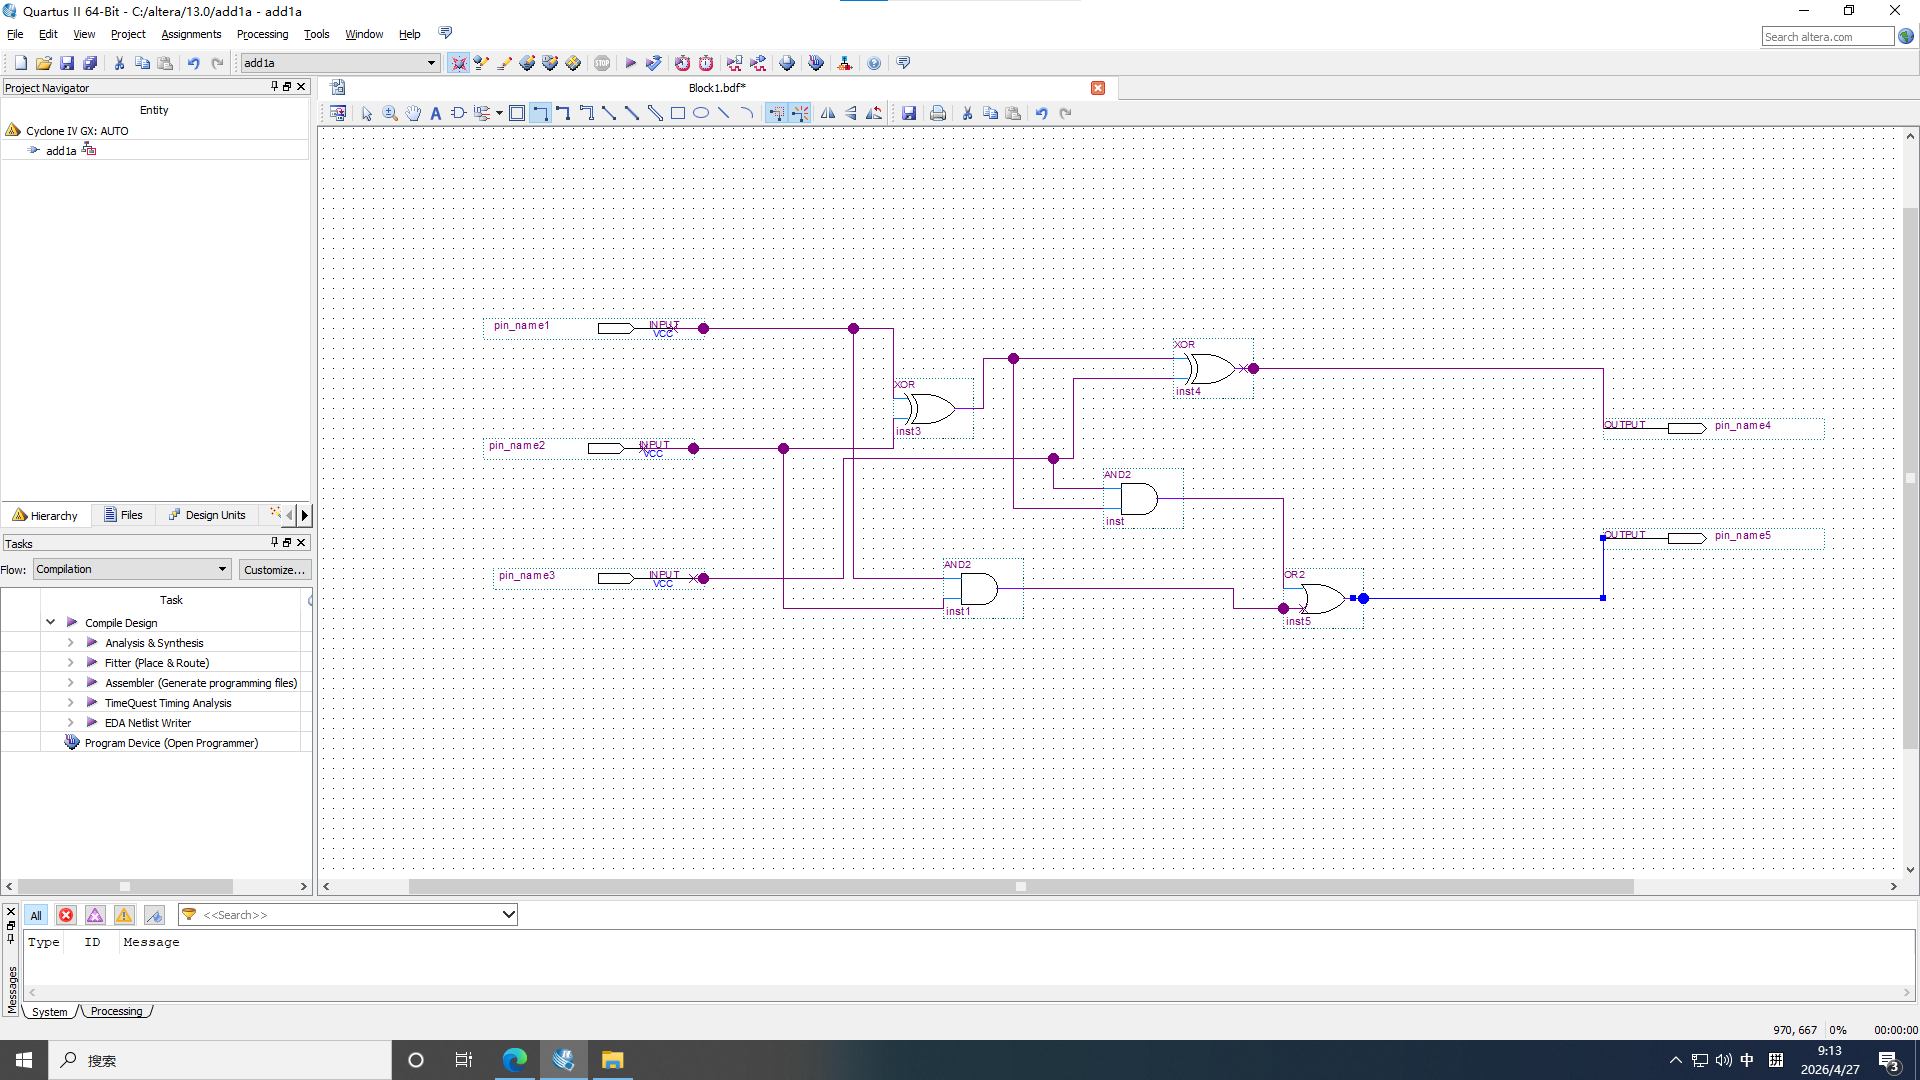
\includegraphics[width=0.75\textwidth]{circuit_diagram.png}
    \caption{一位全加器电路原理图}
    \label{e1:fig:circuit}
\end{figure}

\section{实验内容}

\subsection{创建工程与绘制原理图}

\subsubsection{创建 Quartus II 工程}

启动 Quartus II 软件，通过 \textbf{File $\rightarrow$ New Project Wizard} 创建新工程。在项目信息设置对话框中，设置工程存放路径、项目名称（如 \texttt{add1a}），并确保顶层实体名称与项目名称一致。在目标器件设置中选择 Cyclone V 系列的 \texttt{5CEBA4F23C7} 器件，以匹配 DE0 开发板上的 FPGA 芯片。

\subsubsection{绘制原理图}

工程创建完成后，通过 \textbf{File $\rightarrow$ New $\rightarrow$ Block Diagram/Schematic File} 新建原理图文件。在原理图编辑窗口中，通过元件库（Libraries）放置以下元件：

\begin{itemize}
    \item \texttt{primitives/logic/xor2}：2 个二输入异或门
    \item \texttt{primitives/logic/and2}：2 个二输入与门
    \item \texttt{primitives/logic/or2}：1 个二输入或门
    \item \texttt{primitives/pin/input}：3 个输入引脚（命名为 A、B、C0）
    \item \texttt{primitives/pin/output}：2 个输出引脚（命名为 S、C1）
\end{itemize}

按照图~\ref{e1:fig:circuit} 所示的电路结构连接各元件，完成后保存原理图文件。绘制好的原理图如图~\ref{e1:fig:schematic} 所示。

\begin{figure}[htbp]
    \centering
    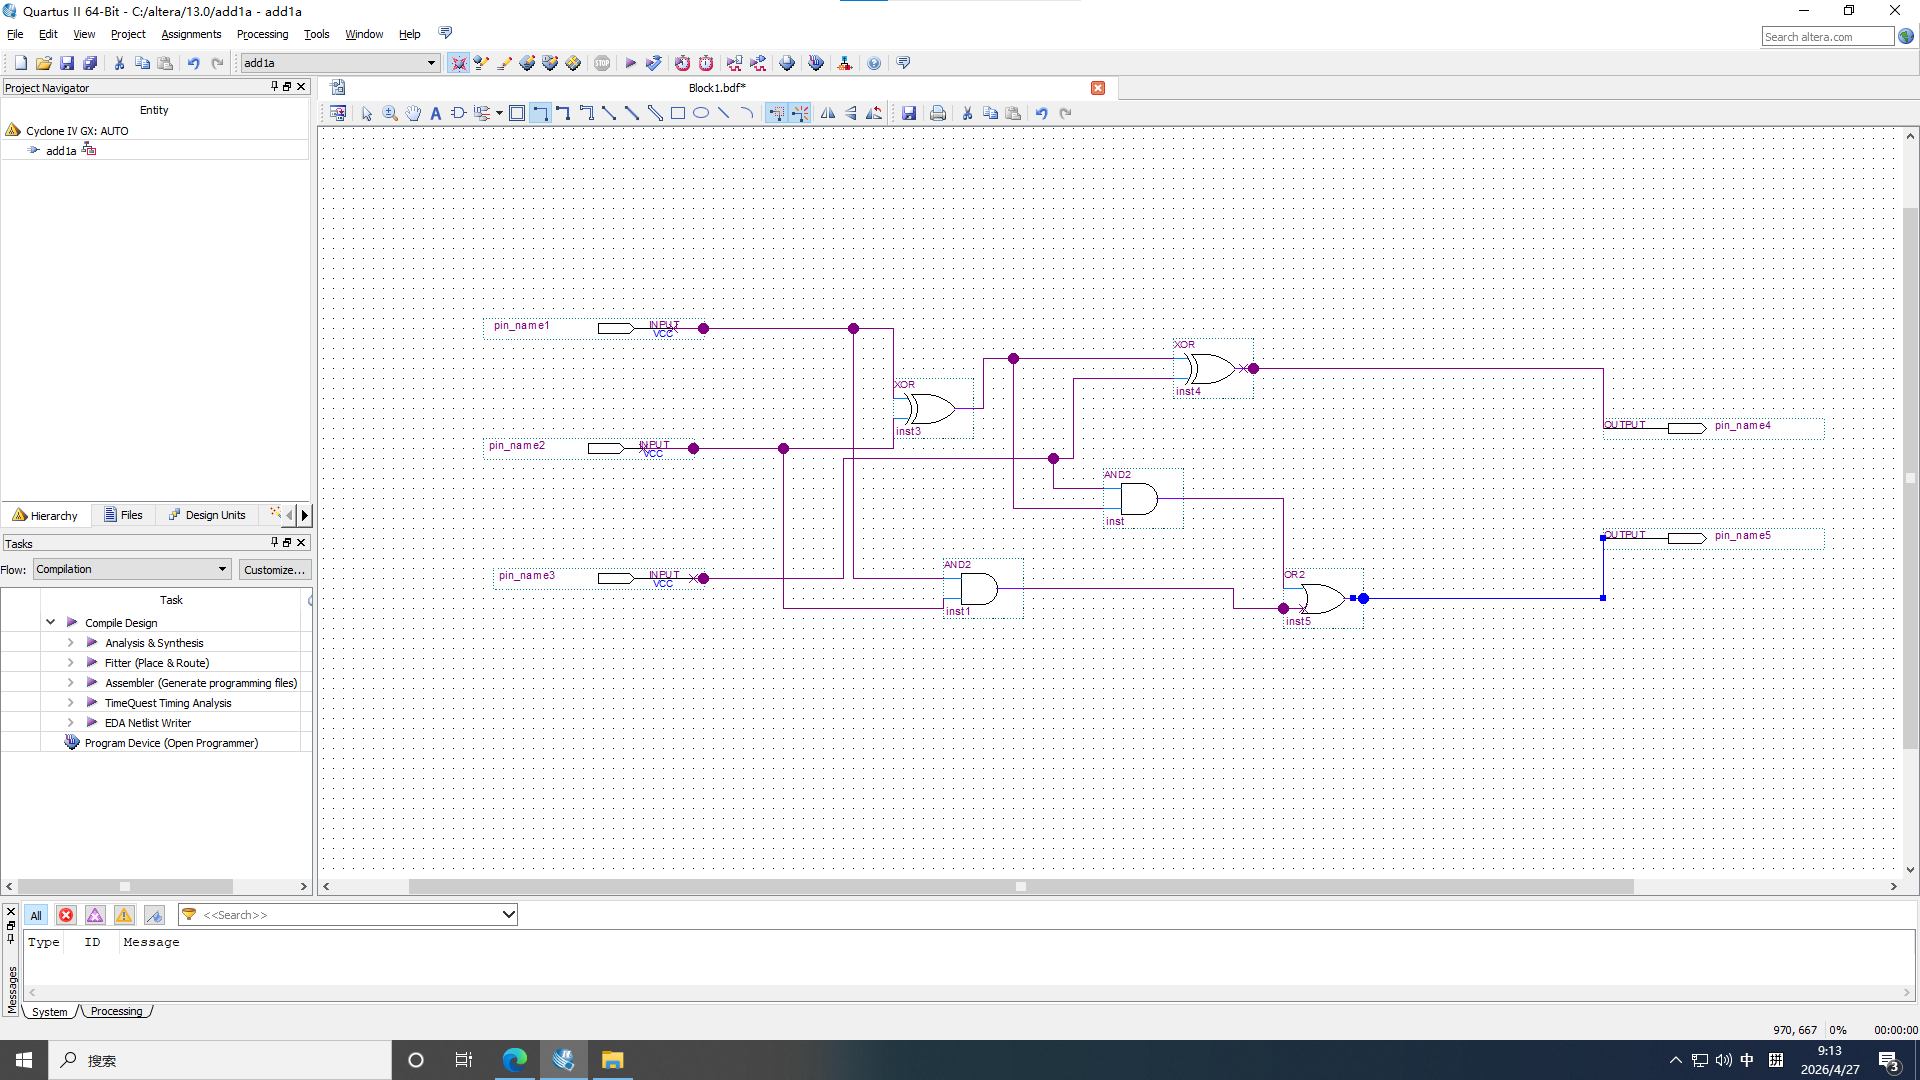
\includegraphics[width=0.75\textwidth]{circuit_diagram.png}
    \caption{Quartus II 中绘制的一位全加器原理图}
    \label{e1:fig:schematic}
\end{figure}

\subsection{编译与波形仿真}

\subsubsection{编译}

原理图绘制完成后，点击工具栏中的编译图标或执行 \textbf{Process $\rightarrow$ Start Compilation} 进行全编译。编译过程包括综合（Synthesis）、适配（Fitter）和汇编（Assembler）等步骤。编译成功后，Quartus II 界面会显示编译报告，确认无错误（Error）即可进行下一步操作。

\subsubsection{波形仿真}

通过 \textbf{File $\rightarrow$ New $\rightarrow$ Verification/Debugging $\rightarrow$ Vector Waveform File} 新建波形仿真文件（.vwf）。使用 \textbf{Edit $\rightarrow$ Insert $\rightarrow$ Insert Node or Bus} 添加仿真信号，在 Node Finder 中选择 \texttt{Pins:all} 获取所有输入输出节点。

设置仿真激励信号的计数值：A 信号每 10ns 翻转一次，B 信号每 20ns 翻转一次，C0 信号每 40ns 翻转一次。这样可以遍历真值表中的所有 8 种输入组合。

执行 \textbf{Processing $\rightarrow$ Start Simulation} 运行仿真，观察输出波形。仿真结果如图~\ref{e1:fig:simulation} 所示。

\begin{figure}[htbp]
    \centering
    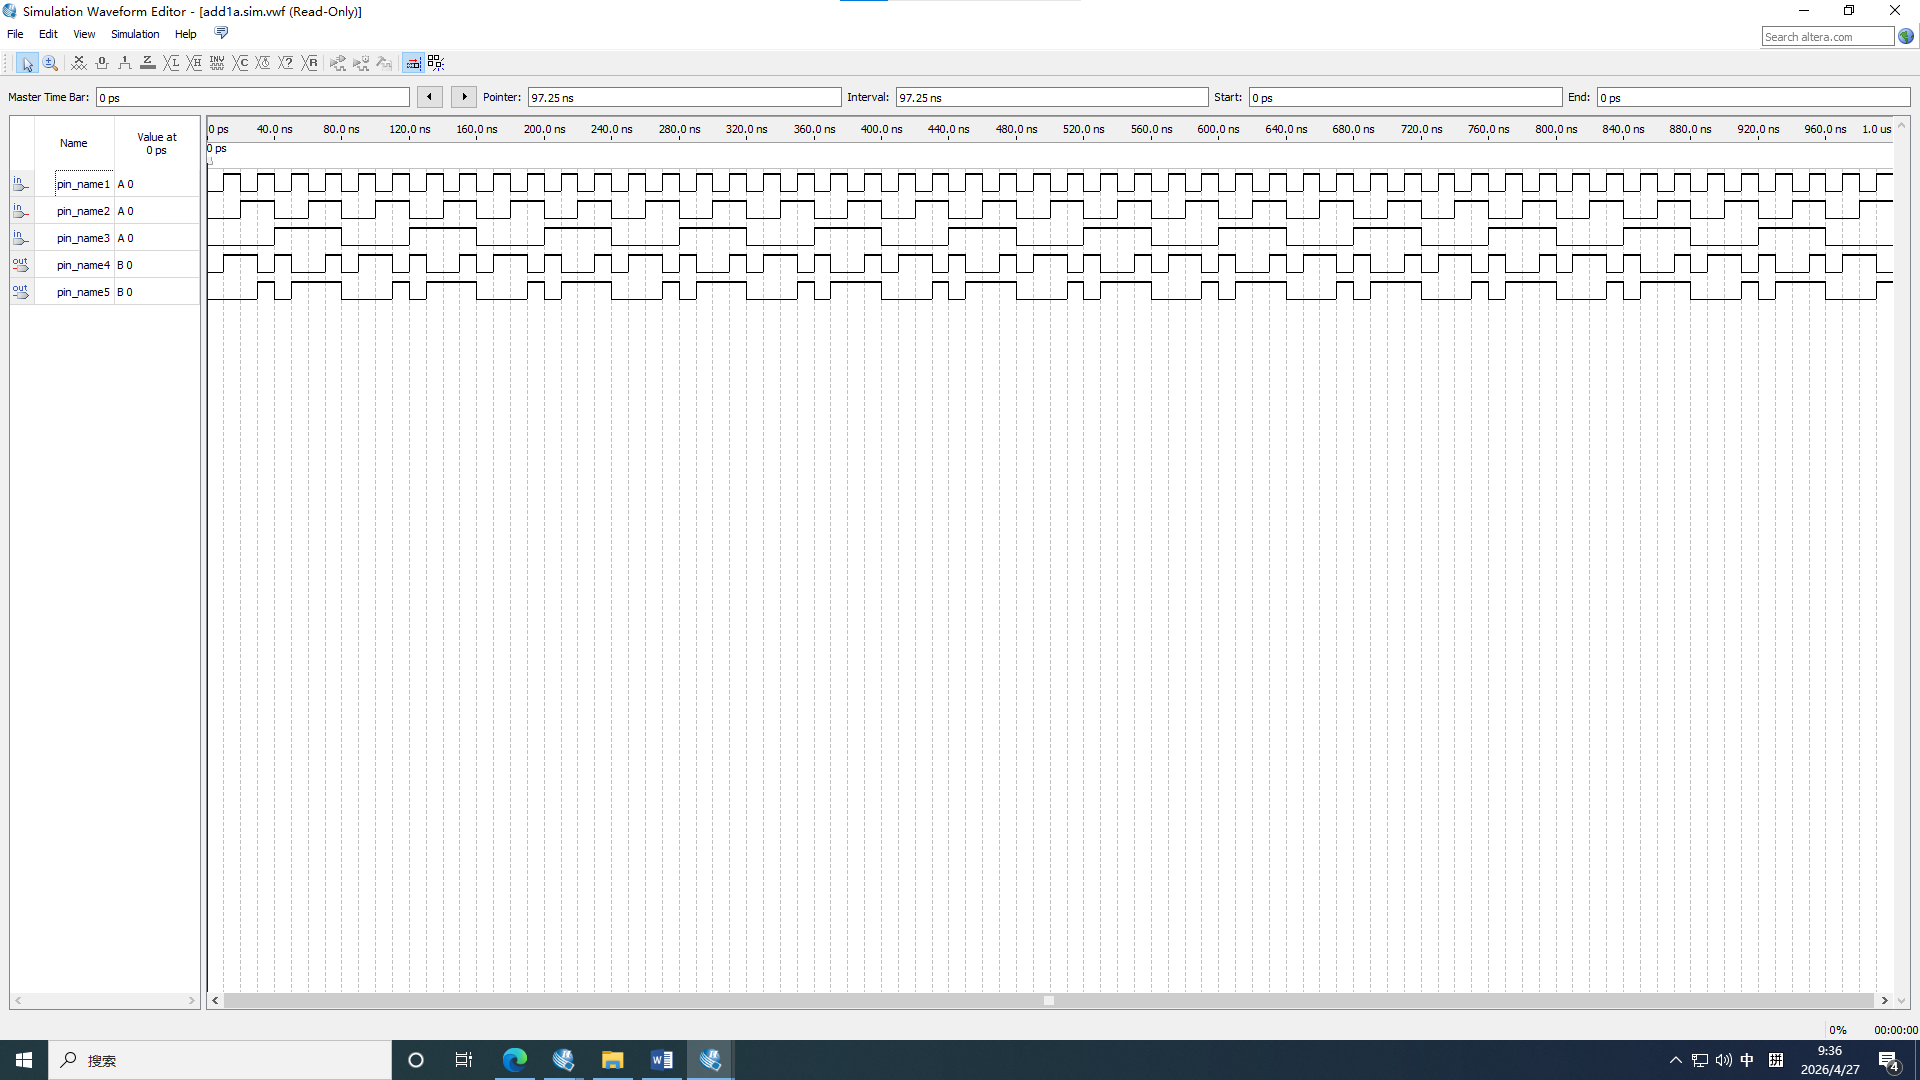
\includegraphics[width=0.75\textwidth]{simulation.png}
    \caption{一位全加器波形仿真结果}
    \label{e1:fig:simulation}
\end{figure}

从仿真波形可以看出，在 0--80ns 的仿真时间内，输入 A、B、C0 的 8 种组合对应的输出 S 和 C1 均与真值表一致，验证了电路设计的正确性。

\subsection{引脚锁定与 FPGA 下载验证}

\subsubsection{引脚锁定}

根据 DE0 开发板的引脚分配表，使用 \textbf{Assignments $\rightarrow$ Pin Planner} 将设计中的端口与 FPGA 物理引脚对应绑定。引脚分配如表~\ref{e1:tab:pin_assign} 所示。

\begin{table}[H]
    \centering
    \caption{引脚分配表}
    \label{e1:tab:pin_assign}
    \begin{tabular}{cccc}
        \toprule
        \textbf{端口名} & \textbf{功能} & \textbf{FPGA 引脚} & \textbf{对应硬件} \\
        \midrule
        A & 输入 & PIN\_U13 & SW0 \\
        B & 输入 & PIN\_V13 & SW1 \\
        C0 & 输入 & PIN\_T13 & SW2 \\
        S & 输出 & PIN\_J1 & LEDG[0] \\
        C1 & 输出 & PIN\_J2 & LEDG[1] \\
        \bottomrule
    \end{tabular}
\end{table}

引脚锁定后，需重新执行全编译以生成包含引脚信息的编程文件（.sof）。

\subsubsection{FPGA 下载}

将计算机通过 USB 线连接至 DE0 开发板的 J8 接口，按下红色电源开关 SW10 启动开发板。在 Quartus II 中执行 \textbf{Tools $\rightarrow$ Programmer}，在编程器对话框中选择 JTAG 模式，点击 \textbf{Hardware Setup} 选择 \texttt{USB-Blaster [USB-0]} 下载接口。加载编译生成的 .sof 文件，勾选 \texttt{Program/Configure}，点击 \textbf{Start} 开始下载。下载成功后的 Programmer 界面如图~\ref{e1:fig:fpga} 所示。

\begin{figure}[htbp]
    \centering
    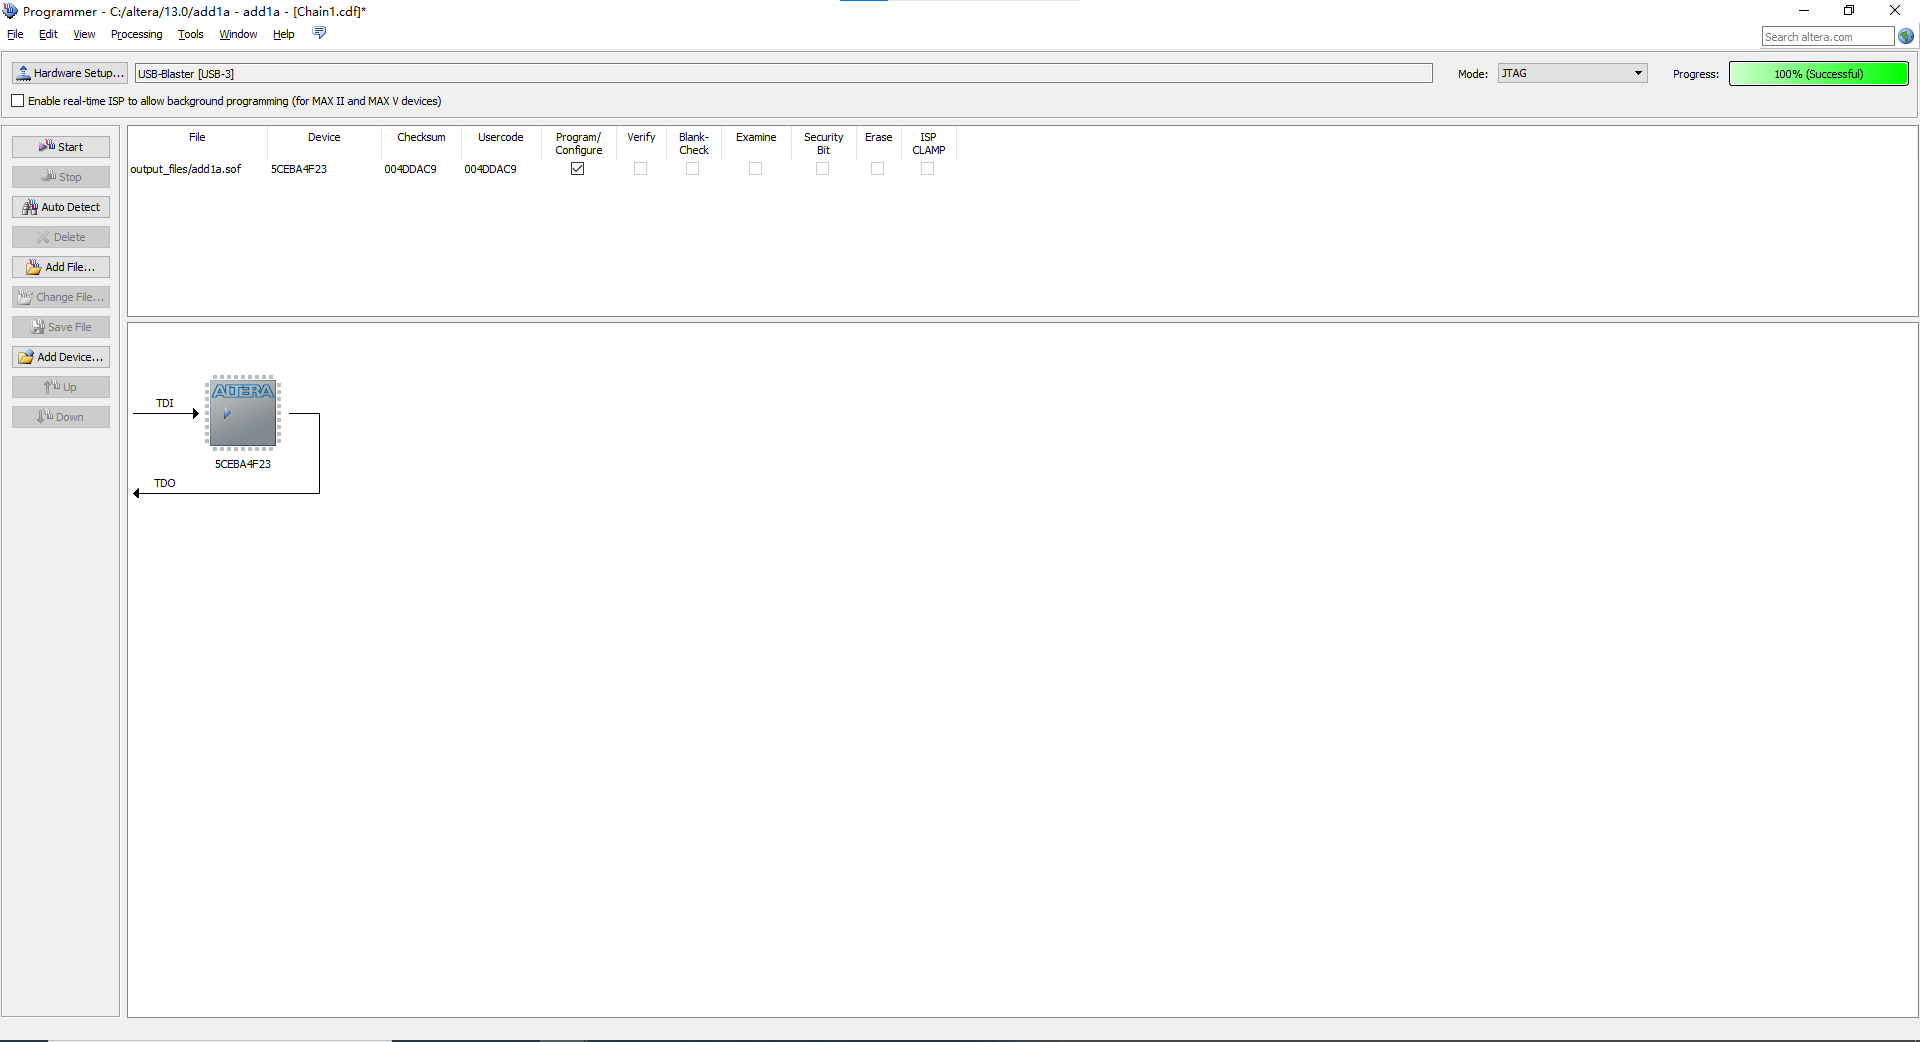
\includegraphics[width=0.7\textwidth]{FPGA.png}
    \caption{FPGA 下载成功界面}
    \label{e1:fig:fpga}
\end{figure}

\subsubsection{硬件验证}

下载完成后，在 DE0 开发板上通过拨动开关 SW0、SW1、SW2 分别控制输入 A、B、C0 的电平，观察 LEDG[0]（S）和 LEDG[1]（C1）的亮灭状态。选取四种典型输入组合进行验证，结果如图~\ref{e1:fig:out00}--\ref{e1:fig:out11} 所示。

\begin{figure}[htbp]
    \centering
    \begin{subfigure}[b]{0.48\textwidth}
        \centering
        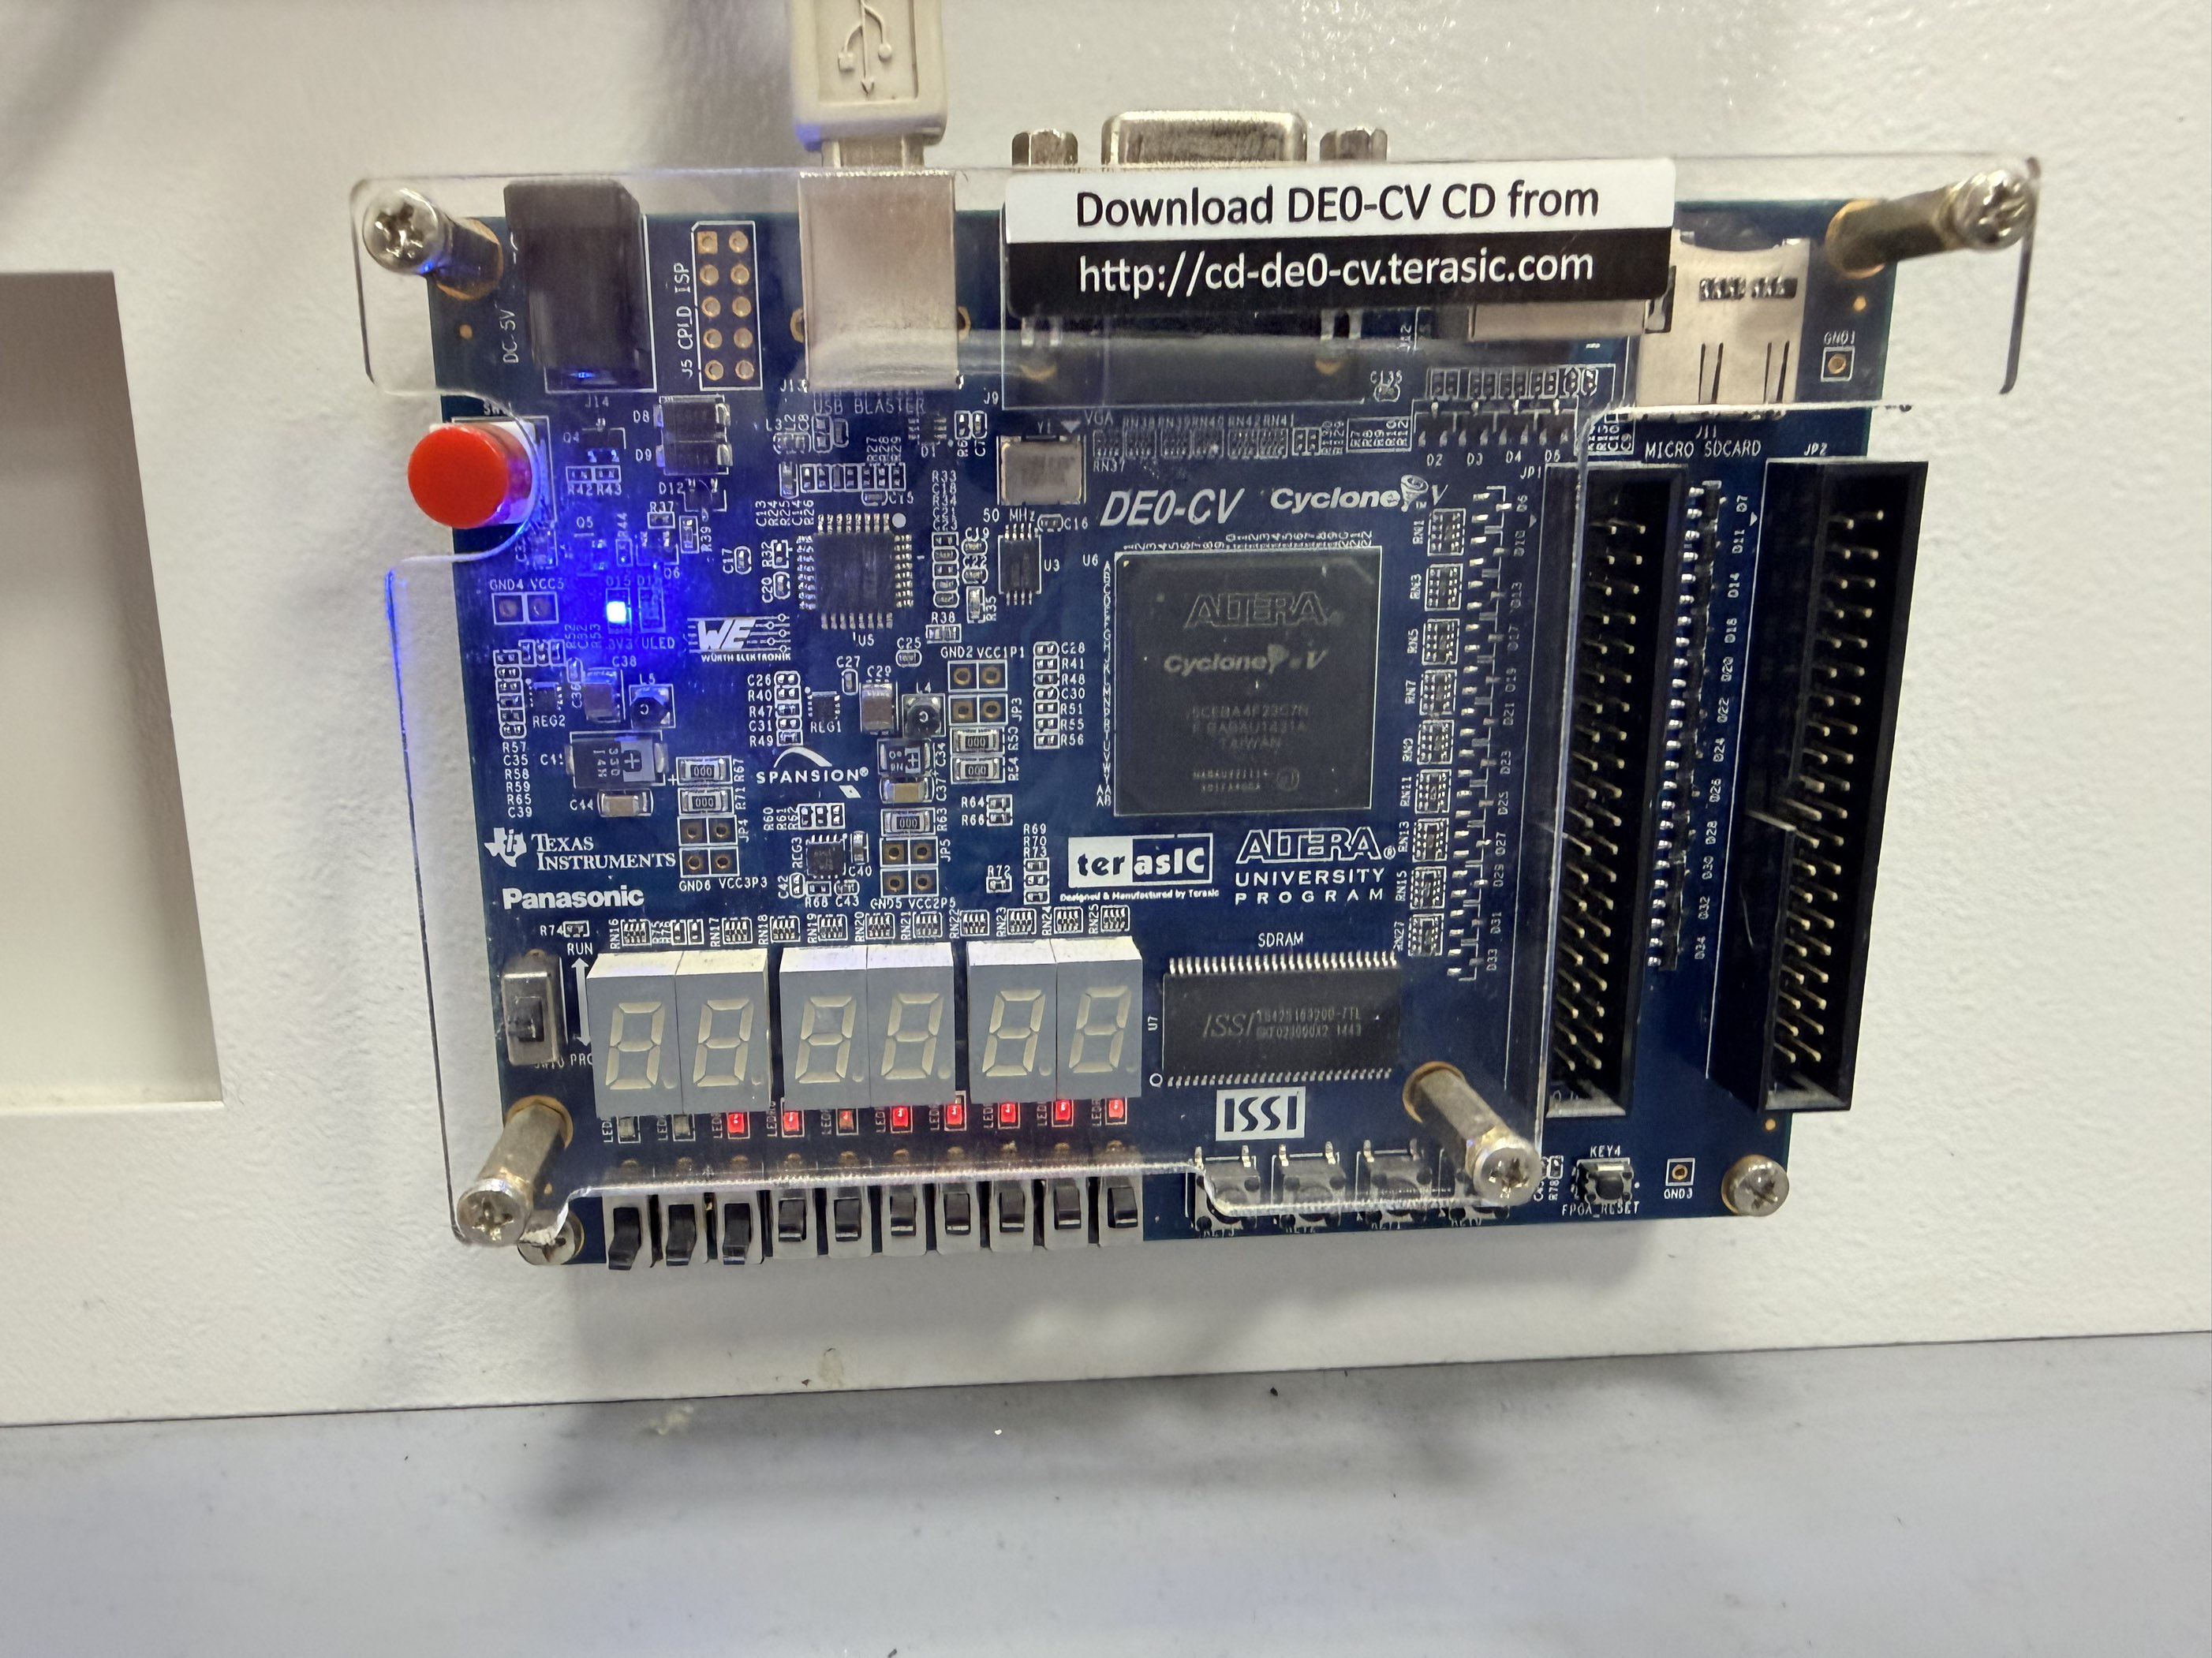
\includegraphics[width=\textwidth]{out00.png}
        \caption{$A=0, B=0, C_0=0 \Rightarrow S=0, C_1=0$}
        \label{e1:fig:out00}
    \end{subfigure}
    \hfill
    \begin{subfigure}[b]{0.48\textwidth}
        \centering
        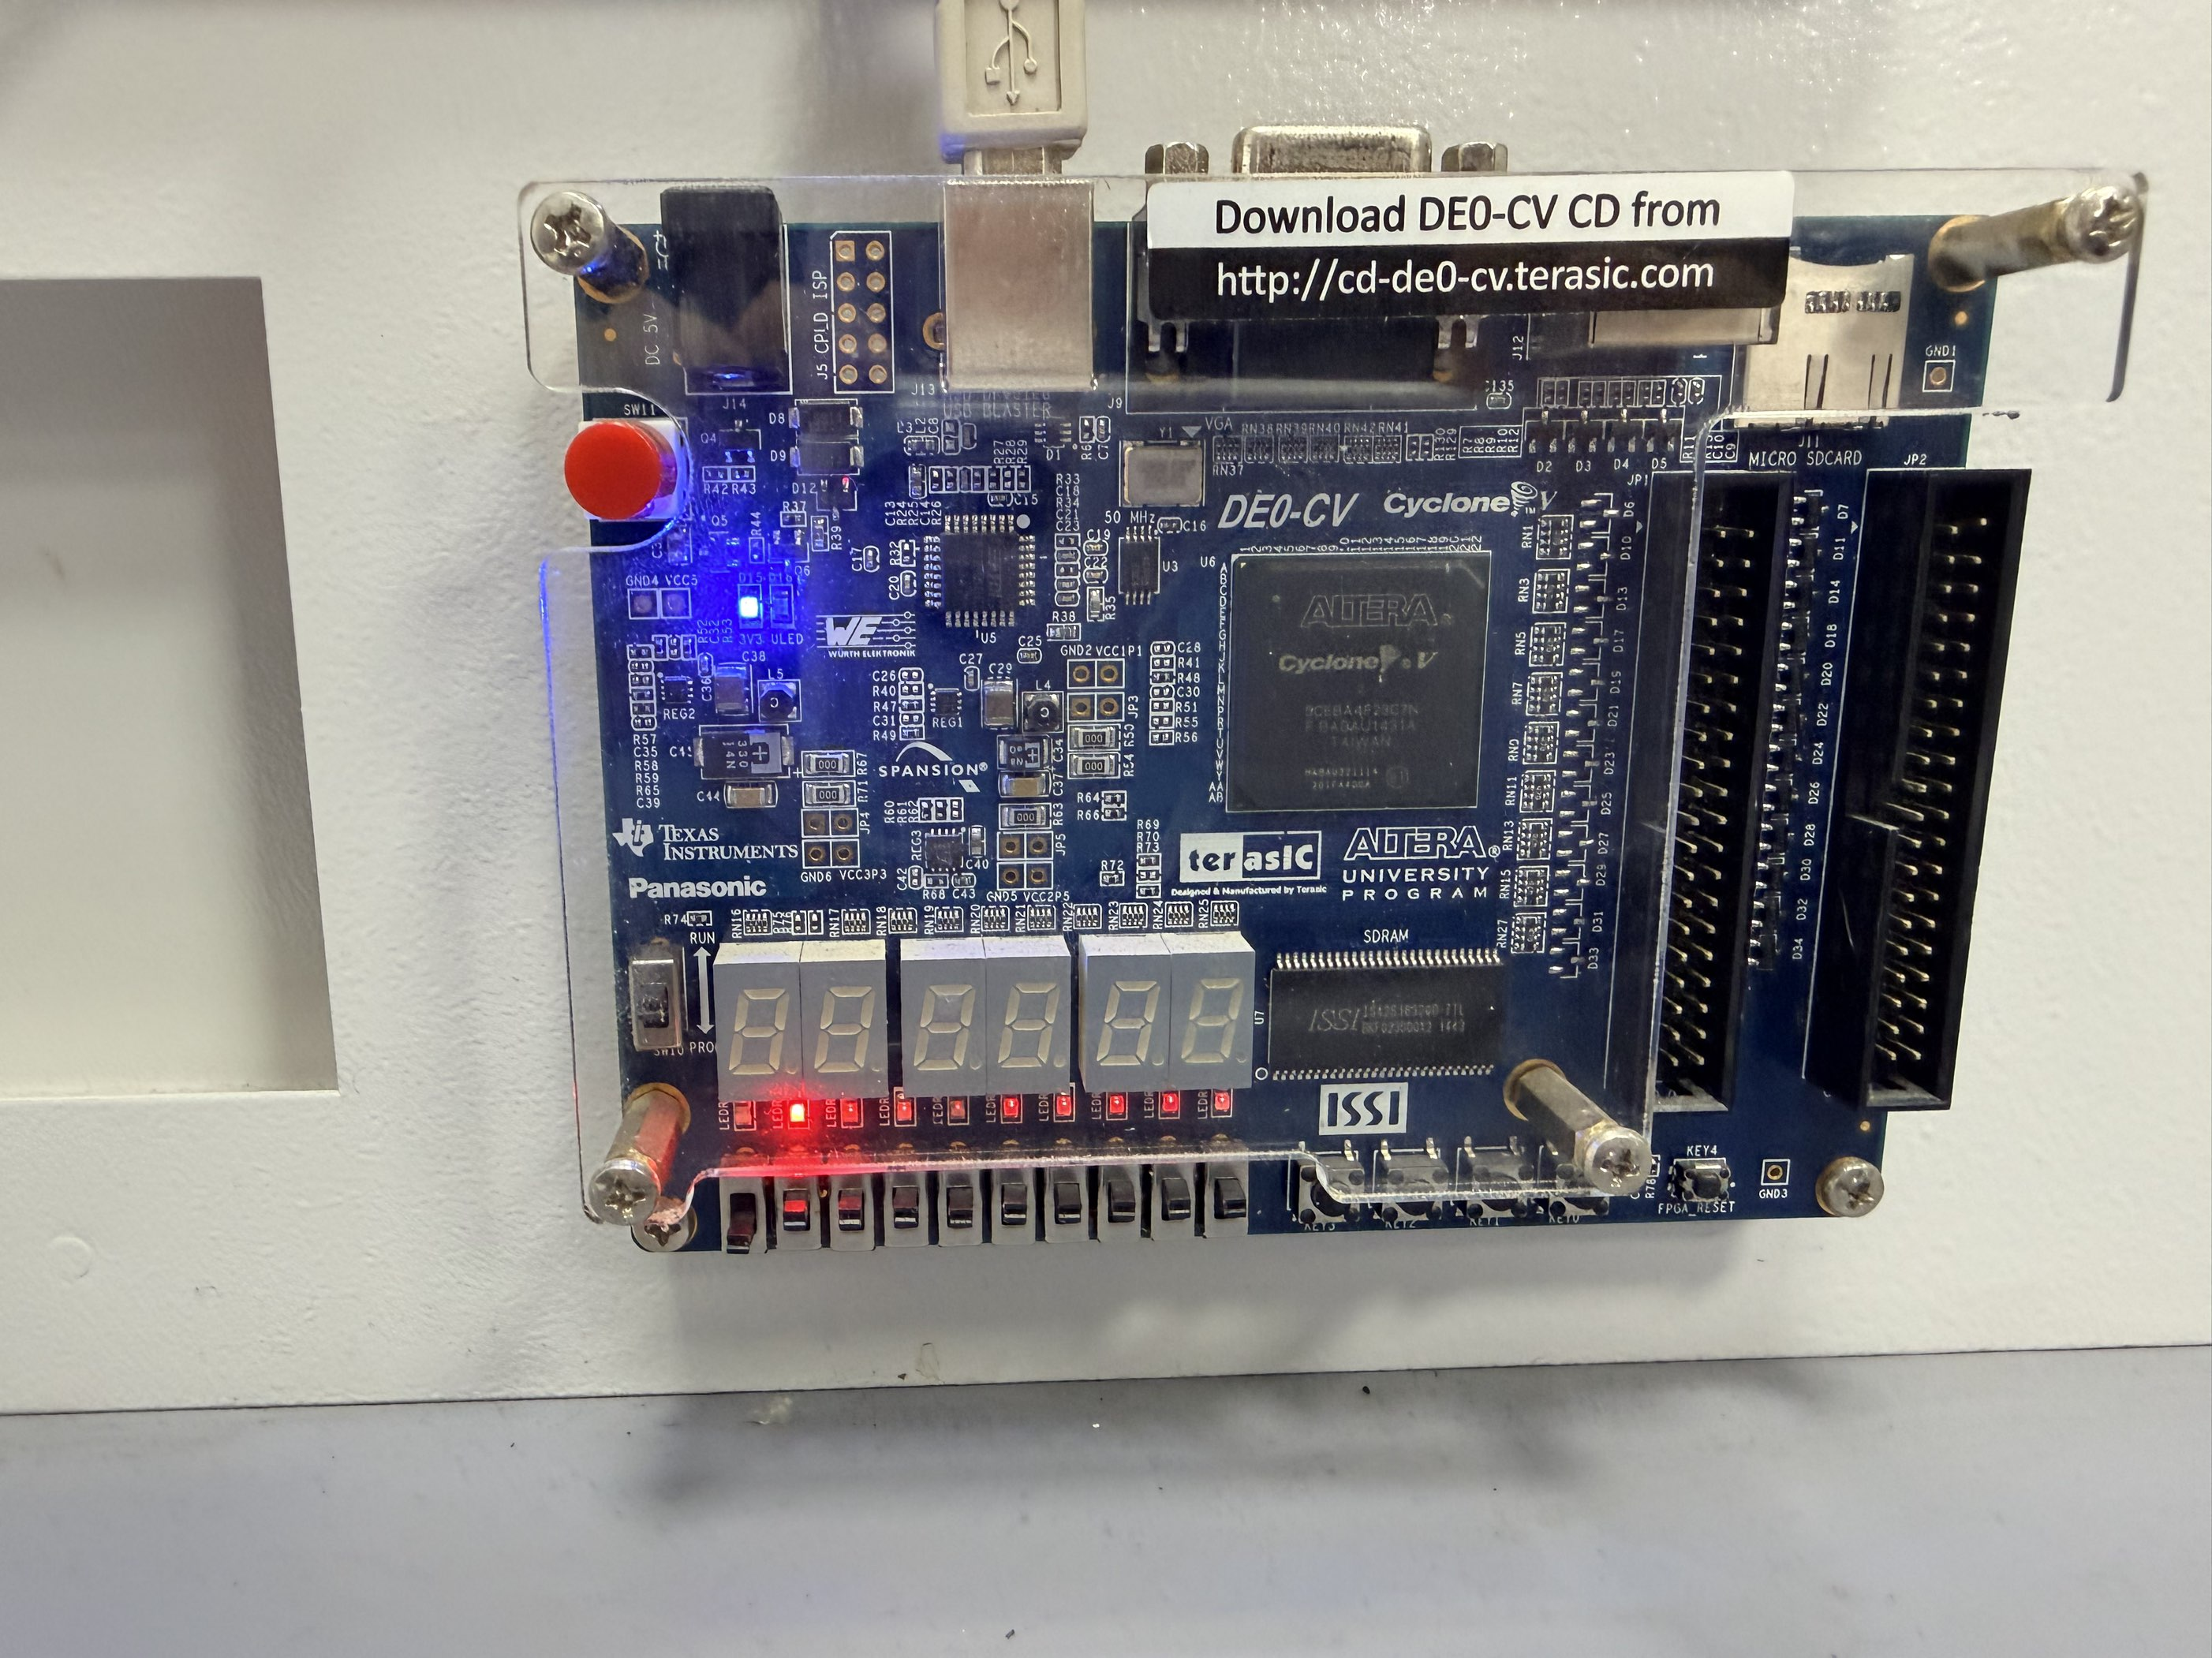
\includegraphics[width=\textwidth]{out01.png}
        \caption{$A=0, B=0, C_0=1 \Rightarrow S=1, C_1=0$}
        \label{e1:fig:out01}
    \end{subfigure}

    \vspace{0.5cm}

    \begin{subfigure}[b]{0.48\textwidth}
        \centering
        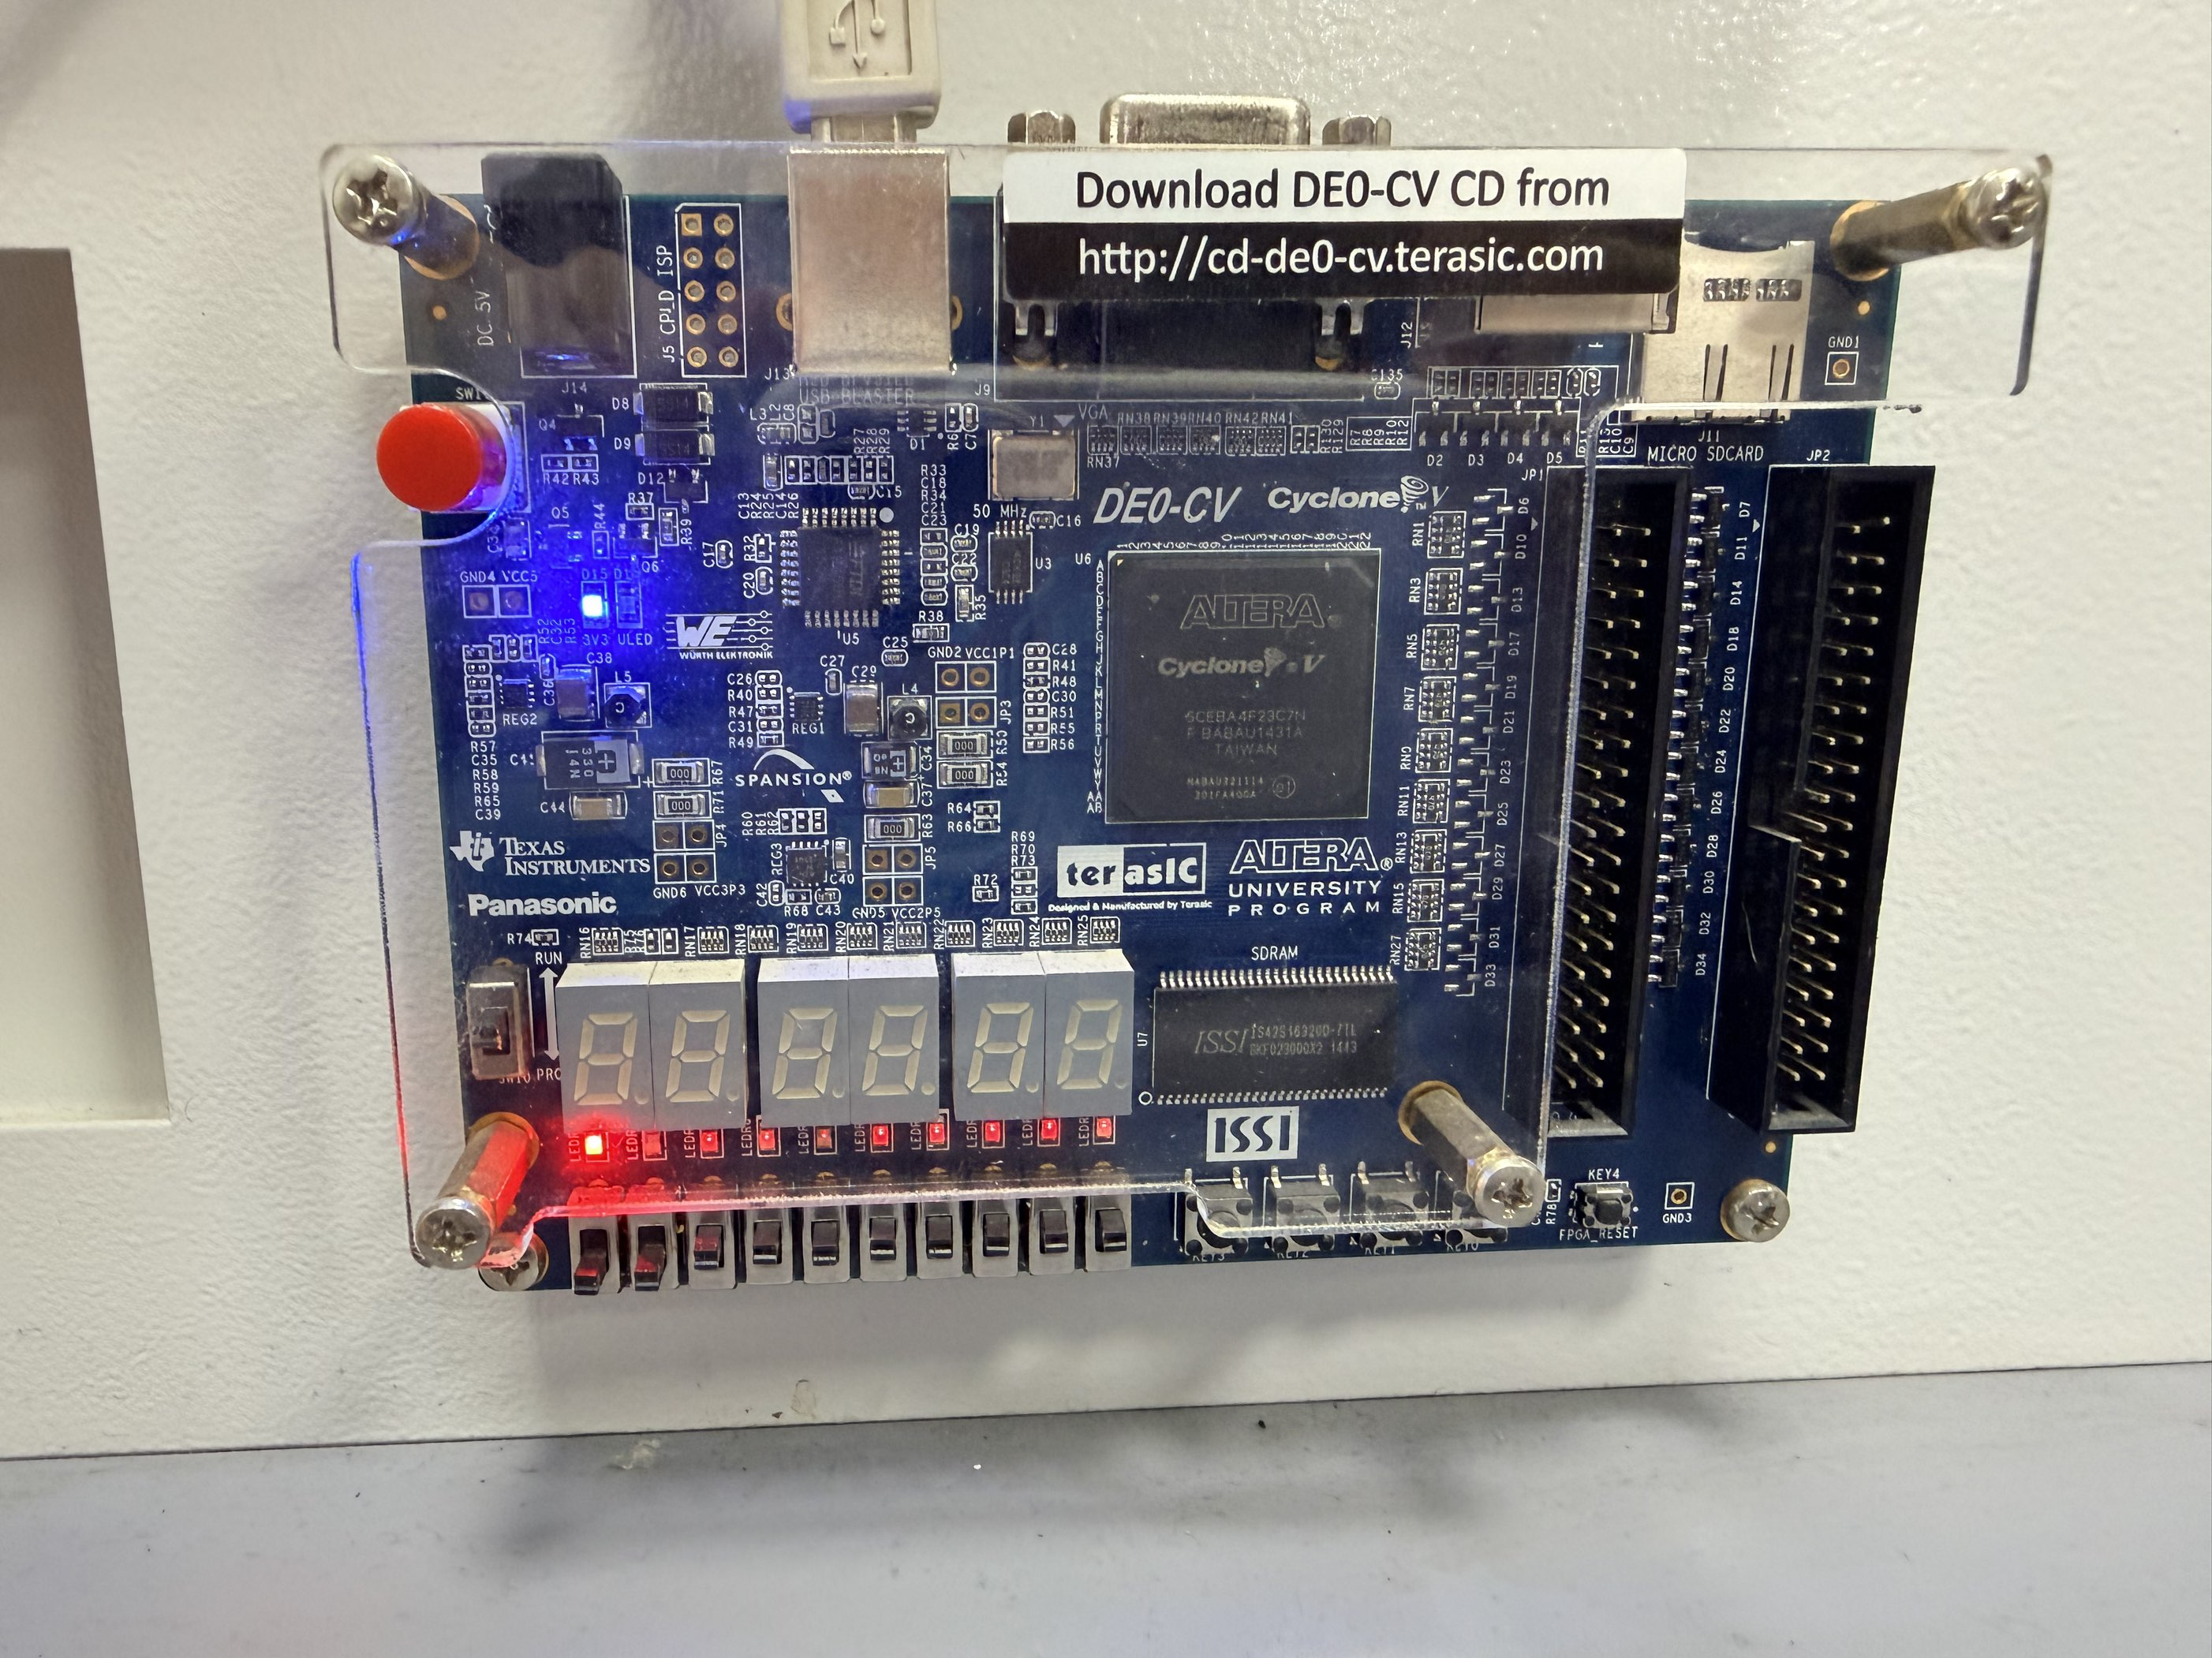
\includegraphics[width=\textwidth]{out10.png}
        \caption{$A=1, B=0, C_0=0 \Rightarrow S=1, C_1=0$}
        \label{e1:fig:out10}
    \end{subfigure}
    \hfill
    \begin{subfigure}[b]{0.48\textwidth}
        \centering
        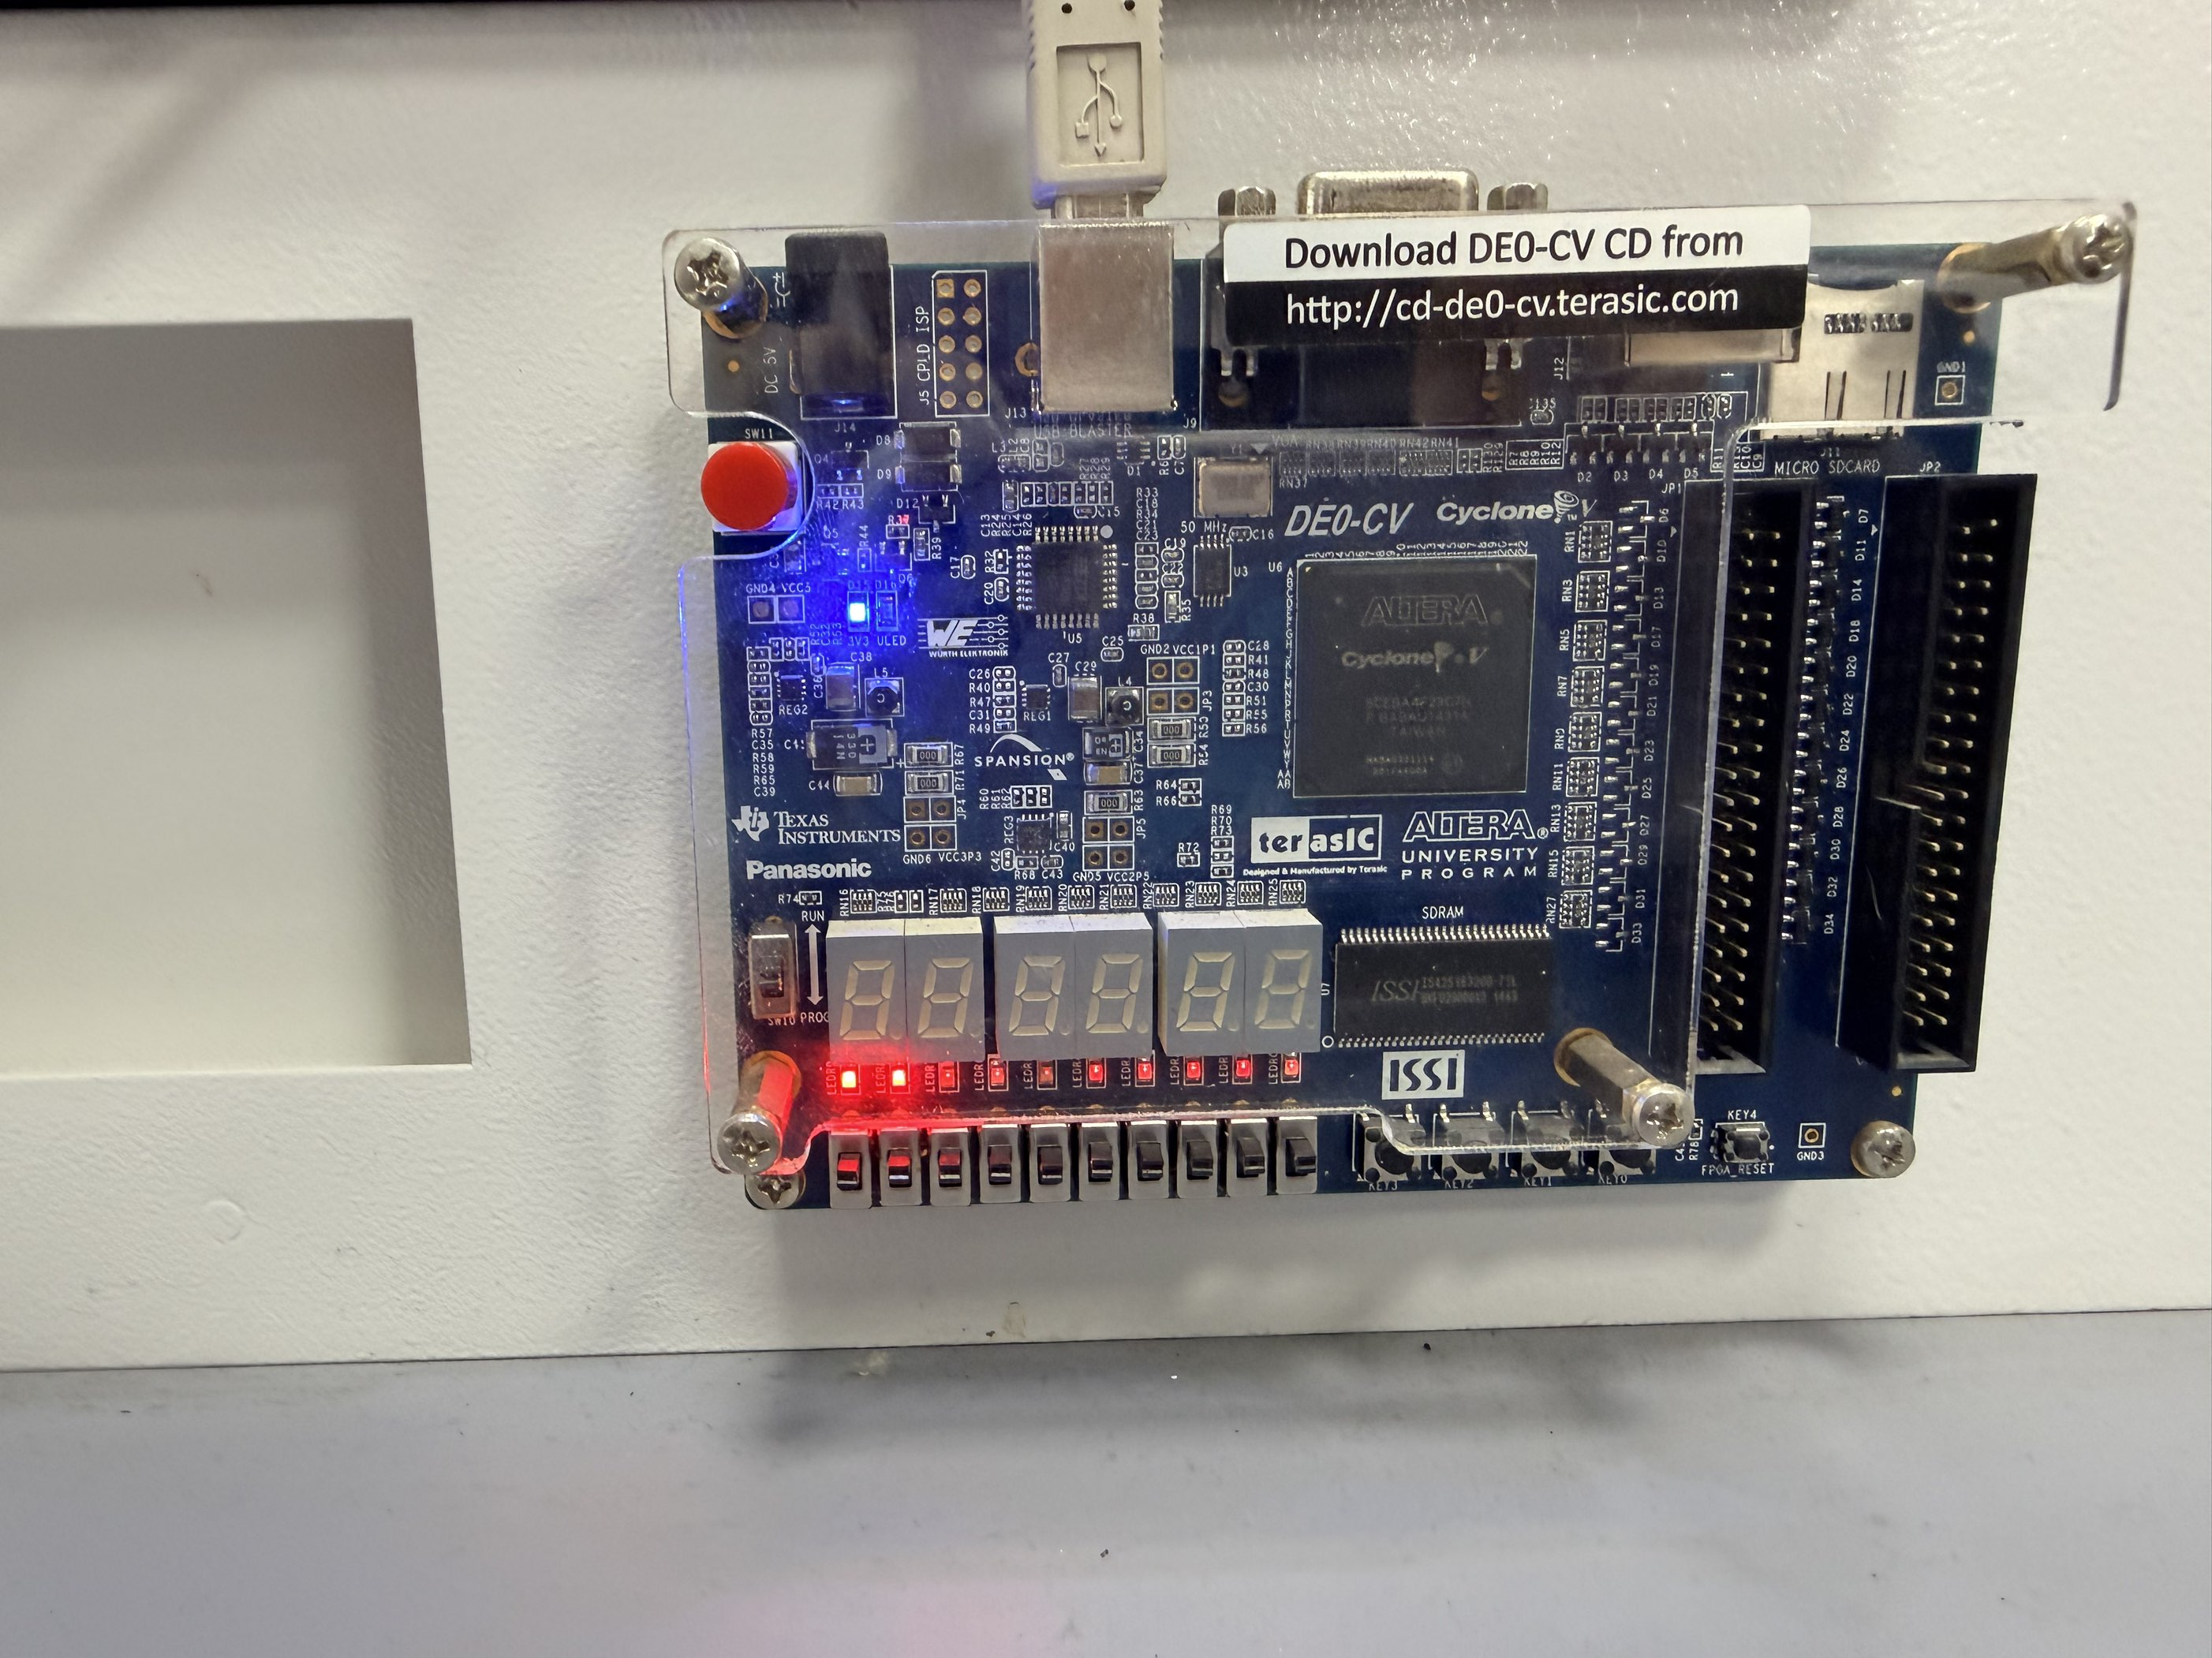
\includegraphics[width=\textwidth]{out11.png}
        \caption{$A=1, B=1, C_0=1 \Rightarrow S=1, C_1=1$}
        \label{e1:fig:out11}
    \end{subfigure}
    \caption{FPGA 硬件验证结果}
    \label{e1:fig:fpga_results}
\end{figure}

从硬件验证结果可以看出，四种输入组合下 LED 灯的亮灭状态均与真值表一致，证明所设计的一位全加器在 FPGA 上正确实现了逻辑功能。

\section{实验过程中的问题}

\begin{enumerate}
    \item \textbf{波形仿真失败}：在首次进行波形仿真时，仿真器报错提示 \texttt{"Can't continue timing simulation because the design has not been successfully compiled for the simulator"}，如图~\ref{e1:fig:sim_fail} 所示。经排查发现，是因为在创建工程时未正确选择目标器件，导致编译产物与仿真器不兼容。重新创建工程并正确选择 Cyclone V 5CEBA4F23C7 器件后，仿真顺利完成。

    \begin{figure}[htbp]
        \centering
        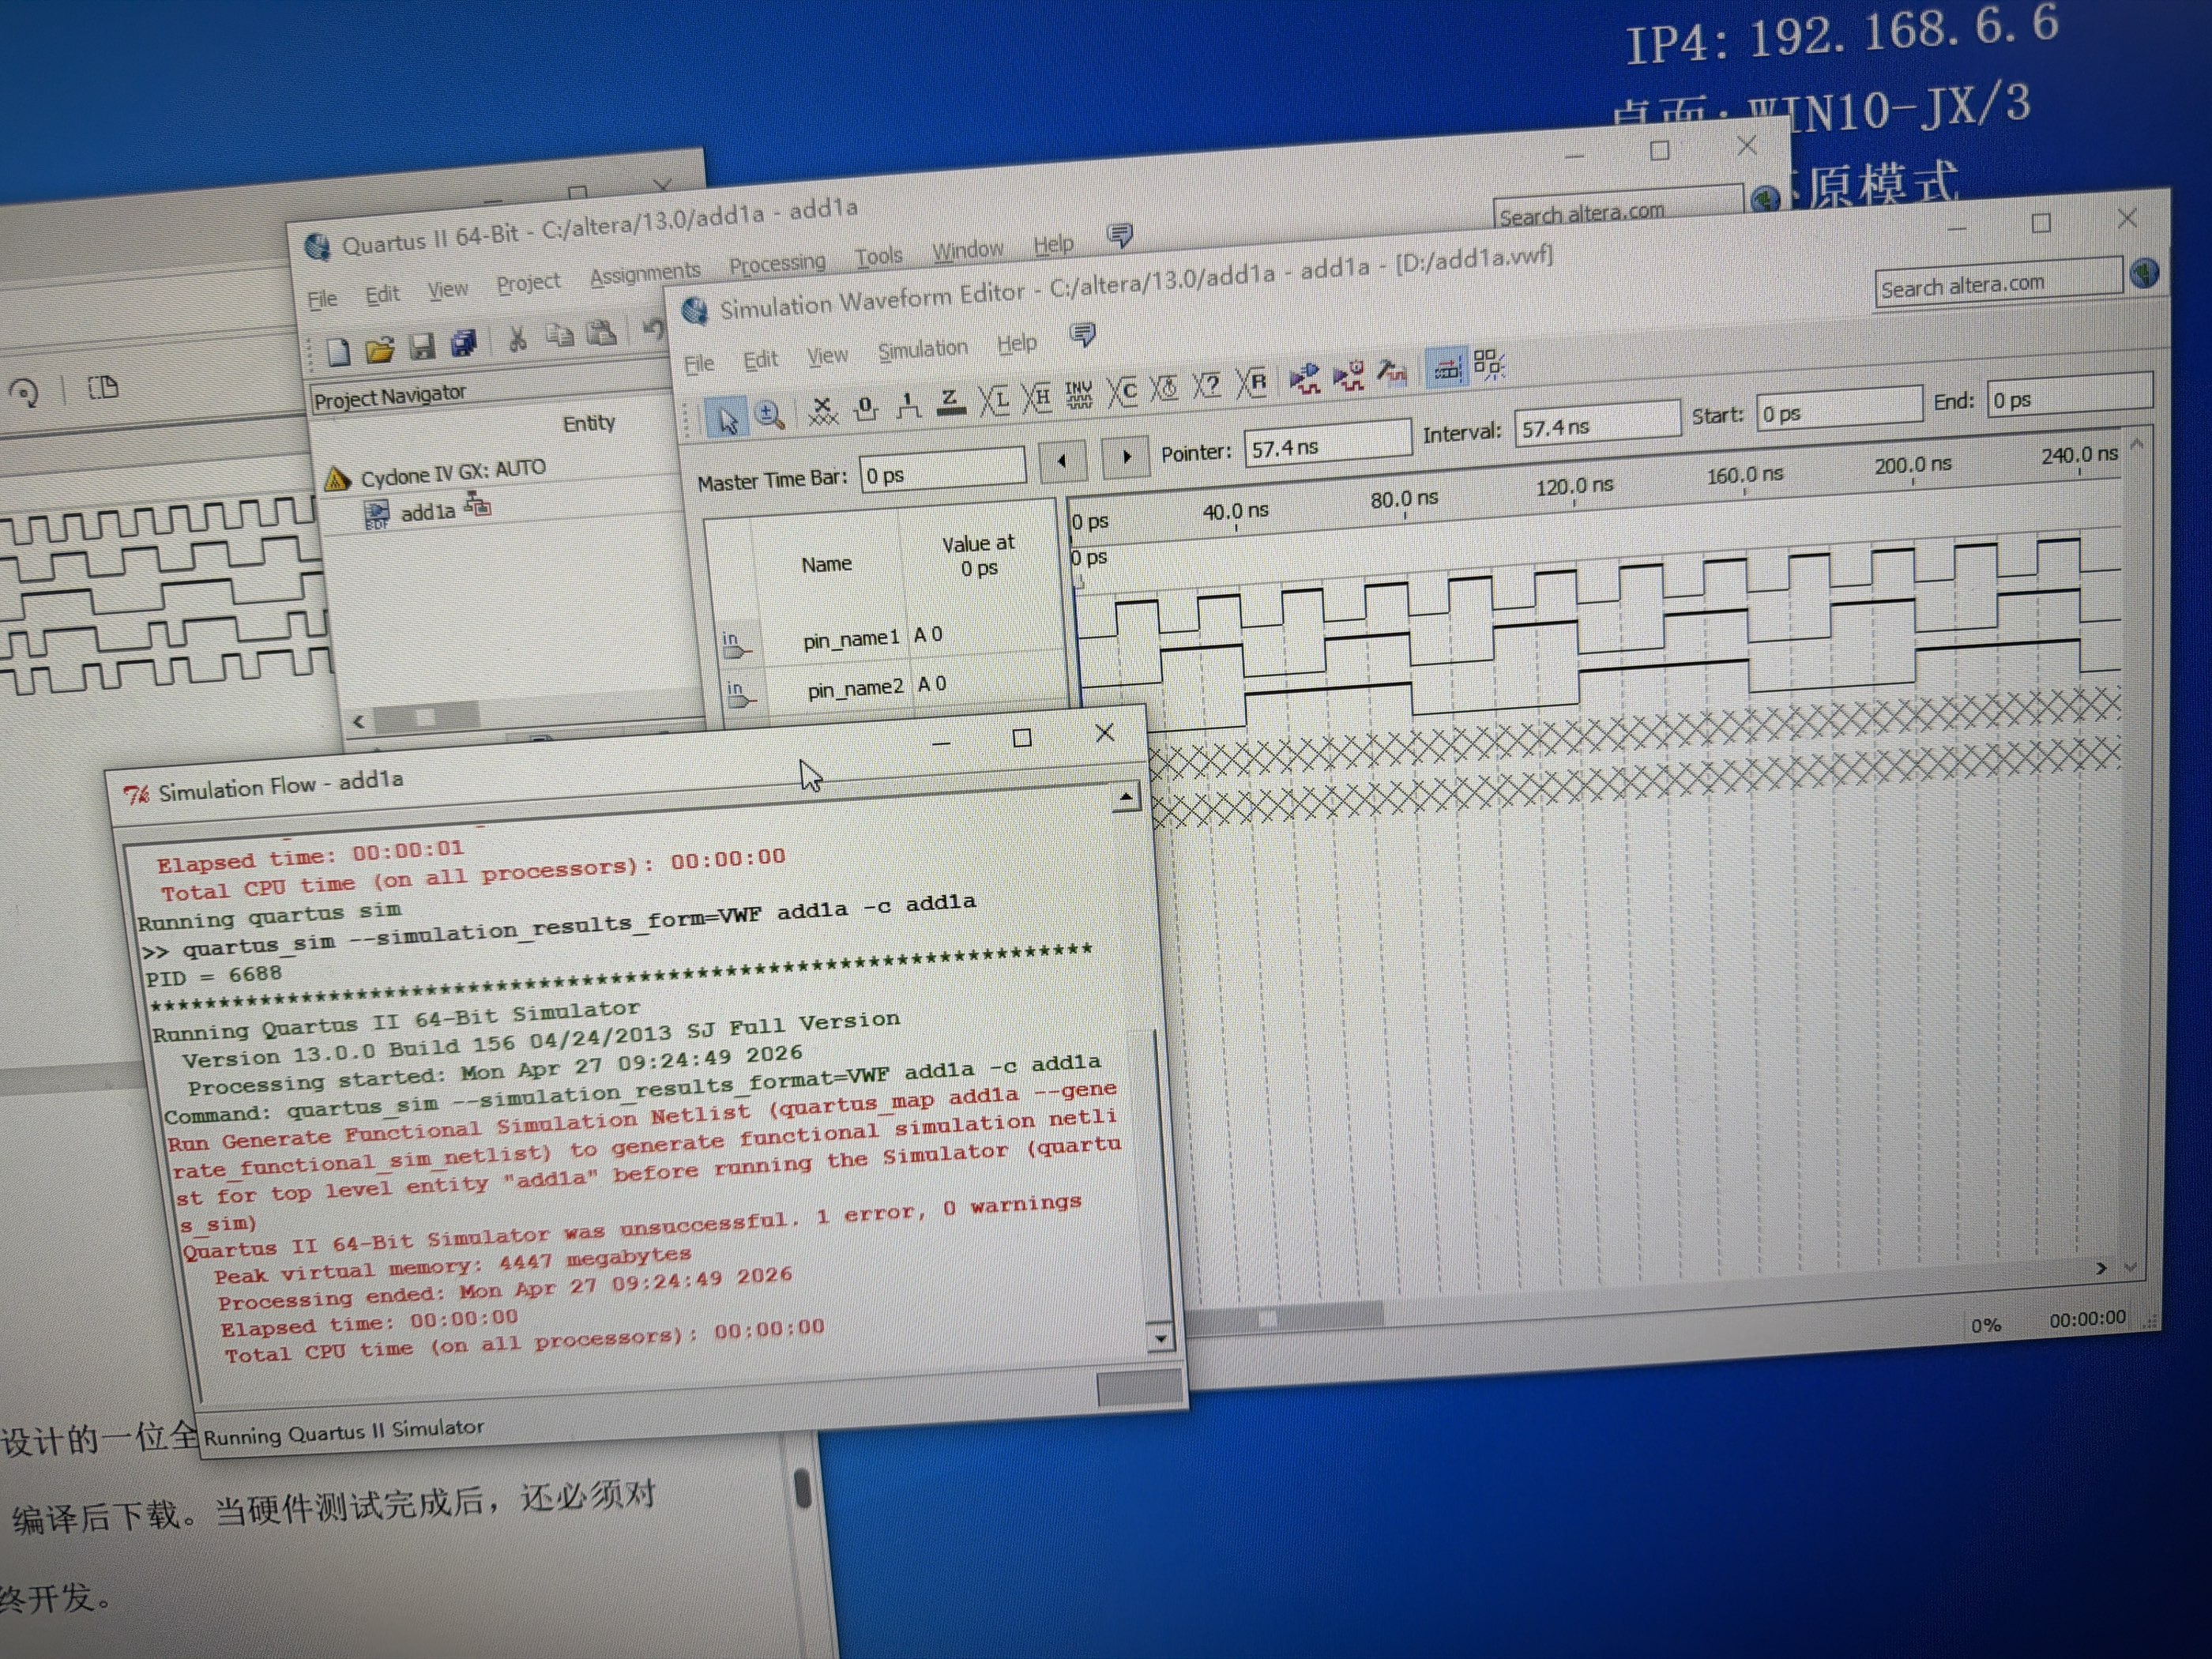
\includegraphics[width=0.7\textwidth]{simulation_fail.png}
        \caption{仿真失败截图（器件选择错误）}
        \label{e1:fig:sim_fail}
    \end{figure}

    \item \textbf{引脚锁定后未重新编译}：在完成引脚锁定后直接进行下载，发现 FPGA 上的 LED 灯输出与预期不符。原因是引脚锁定后需要重新执行全编译，才能将新的引脚信息写入编程文件。重新编译后问题解决。
\end{enumerate}

\section{心得体会}

\begin{enumerate}
    \item 通过本次实验，掌握了使用门电路设计组合逻辑电路的基本方法。从真值表推导逻辑表达式，再到选择合适的门电路实现，整个过程加深了对组合逻辑电路设计的理解。
    \item 学习了 Quartus II 软件的完整设计流程，包括原理图输入、编译、波形仿真、引脚锁定和 FPGA 下载等环节。这些技能为后续更复杂数字电路的设计奠定了基础。
    \item 在实验过程中遇到的仿真失败问题，提醒我在创建工程时必须仔细核对目标器件型号，这是后续所有操作的前提。同时，引脚锁定后需要重新编译这一细节也加深了我对 FPGA 设计流程的理解。
    \item 通过将理论设计与实际硬件验证相结合，直观地感受到了数字电路从设计到实现的完整过程，增强了理论联系实际的能力。
\end{enumerate}

% ==================== 实验2：组合逻辑电路设计 ====================
\graphicspath{{../2. sub/figures/}}
\chapter{组合逻辑电路设计}

\section{实验目的}

\begin{enumerate}
    \item 掌握利用中规模集成组合逻辑器件实现组合逻辑电路的方法。
    \item 学习使用 74153 双四选一数据选择器和 7400 与非门设计一位全减器。
    \item 学习使用 74138 三线八线译码器和与非门设计密码锁电路。
    \item 掌握在 Quartus II 中采用原理图输入、波形仿真、引脚分配和 FPGA 下载验证的基本流程。
    \item 理解多个组合逻辑模块之间的联动控制方法，能够实现密码正确时全减器正常工作的综合功能。
\end{enumerate}

\section{实验要求}

\begin{enumerate}
    \item 使用组合逻辑器件 74153 双四选一数据选择器和 7400 与非门，用原理图输入方法实现一位全减器。
    \item 使用组合逻辑器件 74138 三线八线译码器和与非门，用原理图输入方法实现一个密码锁。密码设为 \texttt{1111}，当密码输入正确时 LED 点亮。
    \item 将密码锁与全减器连接，使密码正确时全减器正常工作；密码错误时，全减器输出被禁止或不表示有效运算结果。
    \item 使用 Quartus II 完成原理图输入、波形仿真，并将设计下载到 DE0 开发板进行验证。
\end{enumerate}

本组两名组员学号最后一位分别为 0 和 9，其四位二进制表示分别为 \texttt{0000} 和 \texttt{1001}；密码正确状态为 \texttt{1111}。

\section{实验设备}

\begin{itemize}
    \item Quartus II 开发软件
    \item DE0 开发板（FPGA 型号：Cyclone V 5CEBA4F23C7）
    \item USB-Blaster 下载线及计算机
    \item 组合逻辑器件符号：74153、74138、7400 及相关输入输出引脚
\end{itemize}

\section{实验原理}

\subsection{一位全减器}

一位全减器用于完成被减数 $A$、减数 $B$ 和来自低位借位 $C_i$ 的一位二进制减法运算，输出差位 $D$ 和向高位借位 $C_o$。其逻辑关系为
\begin{align}
    D &= A \oplus B \oplus C_i, \\
    C_o &= \overline{A}B + \overline{A}C_i + BC_i.
\end{align}

一位全减器真值表如表~\ref{e2:tab:sub_truth} 所示。

\begin{table}[H]
    \centering
    \caption{一位全减器真值表}
    \label{e2:tab:sub_truth}
    \begin{tabular}{ccc|cc}
        \toprule
        $A$ & $B$ & $C_i$ & $D$ & $C_o$ \\
        \midrule
        0 & 0 & 0 & 0 & 0 \\
        0 & 0 & 1 & 1 & 1 \\
        0 & 1 & 0 & 1 & 1 \\
        0 & 1 & 1 & 0 & 1 \\
        1 & 0 & 0 & 1 & 0 \\
        1 & 0 & 1 & 0 & 0 \\
        1 & 1 & 0 & 0 & 0 \\
        1 & 1 & 1 & 1 & 1 \\
        \bottomrule
    \end{tabular}
\end{table}

74153 为双四选一数据选择器，每个数据选择器有两个地址输入和四个数据输入。将变量 $A$、$B$ 作为选择端，把 $C_i$ 或其反变量按真值表接入数据端，即可分别实现差位 $D$ 和借位 $C_o$ 的逻辑函数；再配合 7400 与非门产生所需的反相信号和控制逻辑。

\begin{figure}[htbp]
    \centering
    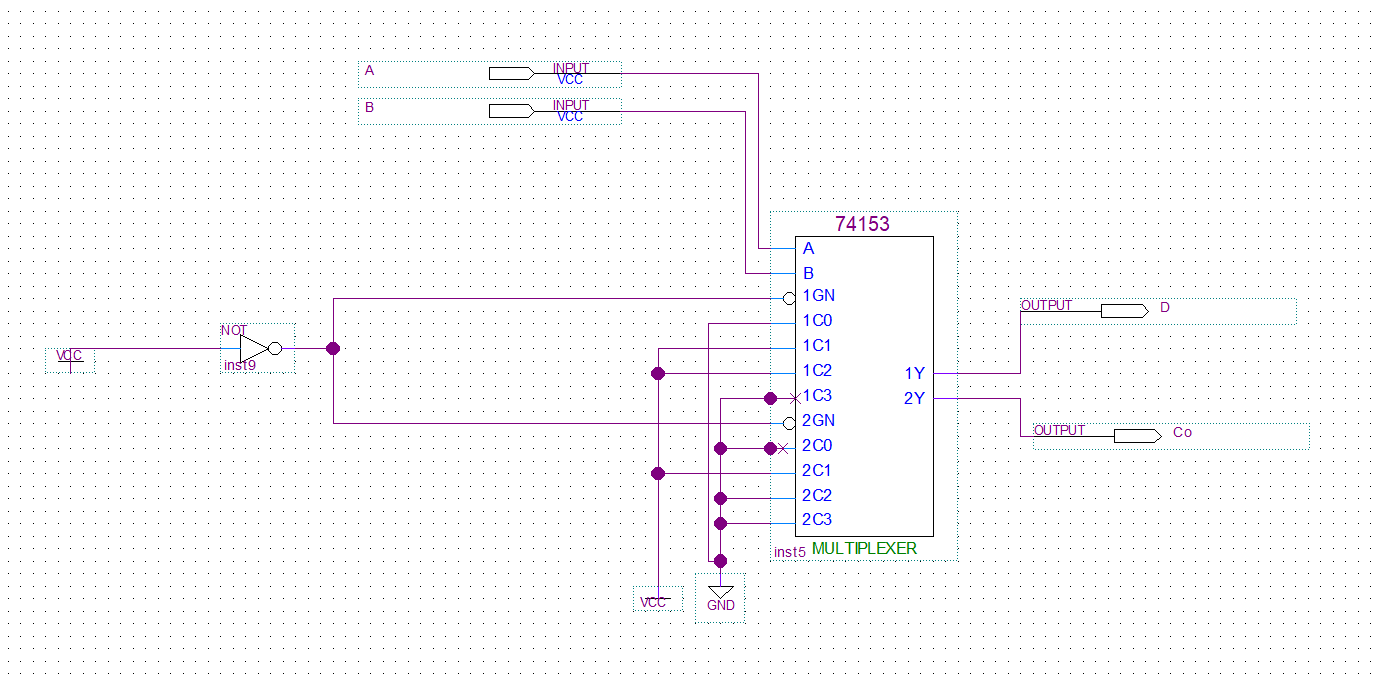
\includegraphics[width=0.75\textwidth]{减法器电路.png}
    \caption{基于 74153 和 7400 的一位全减器原理图}
    \label{e2:fig:sub_circuit}
\end{figure}

\subsection{密码锁电路}

密码锁电路使用 74138 三线八线译码器实现输入状态识别。74138 在使能有效时，根据三位输入选择一个低有效输出端。由于实验密码为 \texttt{1111}，可将四位密码输入拆分为译码输入和使能控制：当高位条件和低三位译码结果同时满足时，通过与非门组合得到密码正确标志信号。

对于本组输入，学号末位 0 和 9 可分别表示为 \texttt{0000} 和 \texttt{1001}。实验中以 \texttt{1111} 作为密码正确状态，并用 LED 显示密码锁判断结果。

\begin{figure}[htbp]
    \centering
    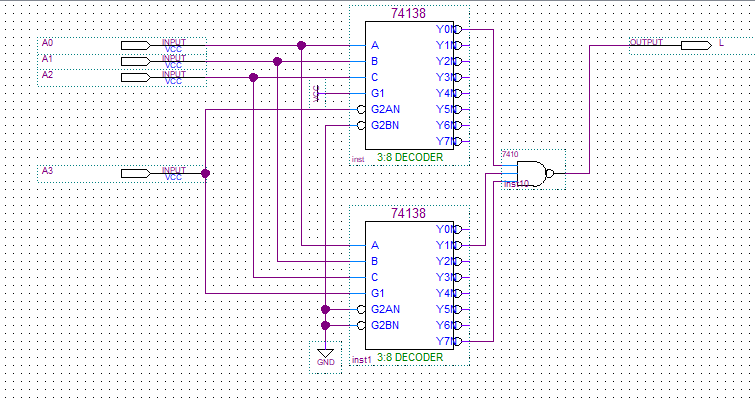
\includegraphics[width=0.75\textwidth]{密码锁电路.png}
    \caption{基于 74138 和与非门的密码锁原理图}
    \label{e2:fig:lock_circuit}
\end{figure}

\subsection{全减器与密码锁联动}

将密码锁输出作为全减器模块的有效控制信号。当密码输入为 \texttt{1111} 时，控制信号有效，全减器输出差位和借位；当密码输入不正确时，控制信号无效，最终输出不作为有效减法结果。通过这种方式可验证组合逻辑模块的级联设计方法。

\begin{figure}[htbp]
    \centering
    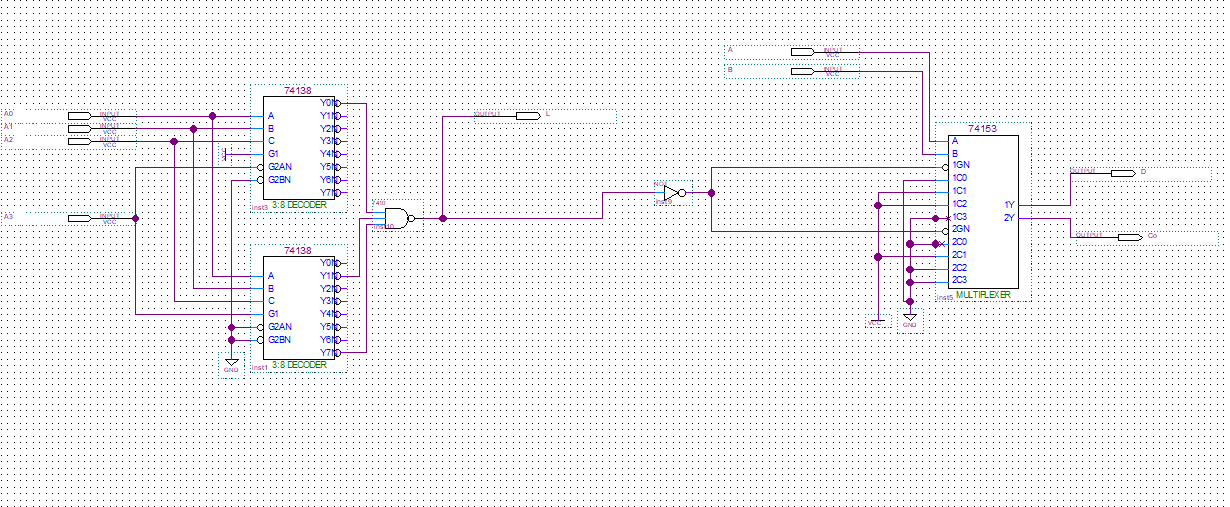
\includegraphics[width=0.75\textwidth]{最终电路.png}
    \caption{密码锁控制全减器工作的最终联动电路}
    \label{e2:fig:final_circuit}
\end{figure}

\section{实验内容}

\subsection{工程创建与原理图输入}

启动 Quartus II，通过 \textbf{File $\rightarrow$ New Project Wizard} 创建实验二工程。在器件选择中指定 Cyclone V 系列的 \texttt{5CEBA4F23C7}，与 DE0 开发板保持一致。新建 Block Diagram/Schematic File 后，分别放置 74153、74138、7400、输入引脚和输出引脚，并按实验要求完成全减器、密码锁和最终联动电路的连接。

\subsection{一位全减器设计与仿真}

全减器部分使用 74153 的选择功能实现 $D$ 和 $C_o$ 两个输出。输入端 $A$、$B$ 和 $C_i$ 通过拨动开关给出，输出差位和借位连接到 LED。完成原理图后进行全编译，并建立波形仿真文件验证 8 种输入组合下输出是否与真值表一致。

\begin{figure}[htbp]
    \centering
    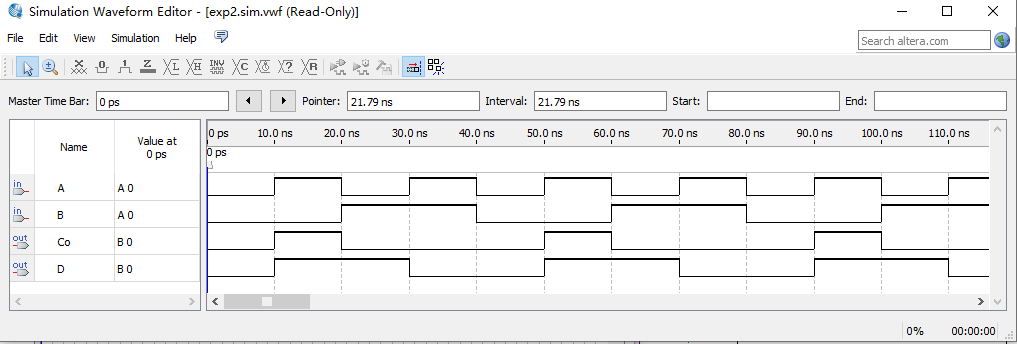
\includegraphics[width=0.75\textwidth]{减法器仿真波形.png}
    \caption{一位全减器波形仿真结果}
    \label{e2:fig:sub_wave}
\end{figure}

由图~\ref{e2:fig:sub_wave} 可见，随着 $A$、$B$、$C_i$ 按不同组合变化，输出差位 $D$ 和借位 $C_o$ 能够对应全减器真值表变化，说明全减器模块逻辑正确。

\subsection{密码锁设计与仿真}

密码锁部分使用 74138 对输入状态进行译码，并使用与非门组合得到密码正确信号。设置密码为 \texttt{1111}，当密码输入满足该状态时，密码锁输出有效并驱动对应 LED；当输入为其他状态时，密码锁输出无效。

\begin{figure}[htbp]
    \centering
    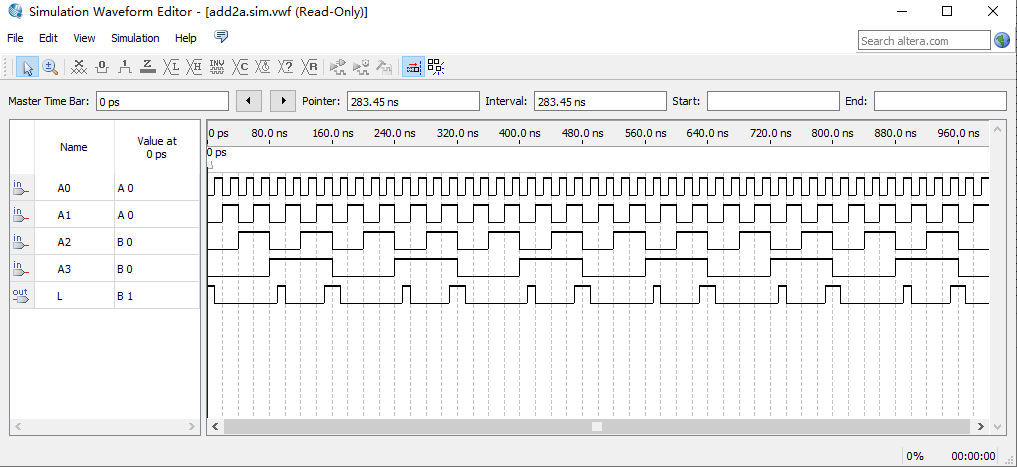
\includegraphics[width=0.75\textwidth]{密码锁仿真波形.png}
    \caption{密码锁波形仿真结果}
    \label{e2:fig:lock_wave}
\end{figure}

由图~\ref{e2:fig:lock_wave} 可见，当输入密码为 \texttt{1111} 时，密码正确标志信号有效；其他输入状态下，标志信号保持无效，满足密码锁设计要求。

\subsection{联动电路设计与仿真}

在最终电路中，将密码锁输出接入全减器控制端。仿真时先改变密码输入，观察密码正确标志；再在密码正确状态下改变全减器输入，观察差位和借位是否正常变化。这样可以同时验证密码锁判断和全减器运算两个功能。

\begin{figure}[htbp]
    \centering
    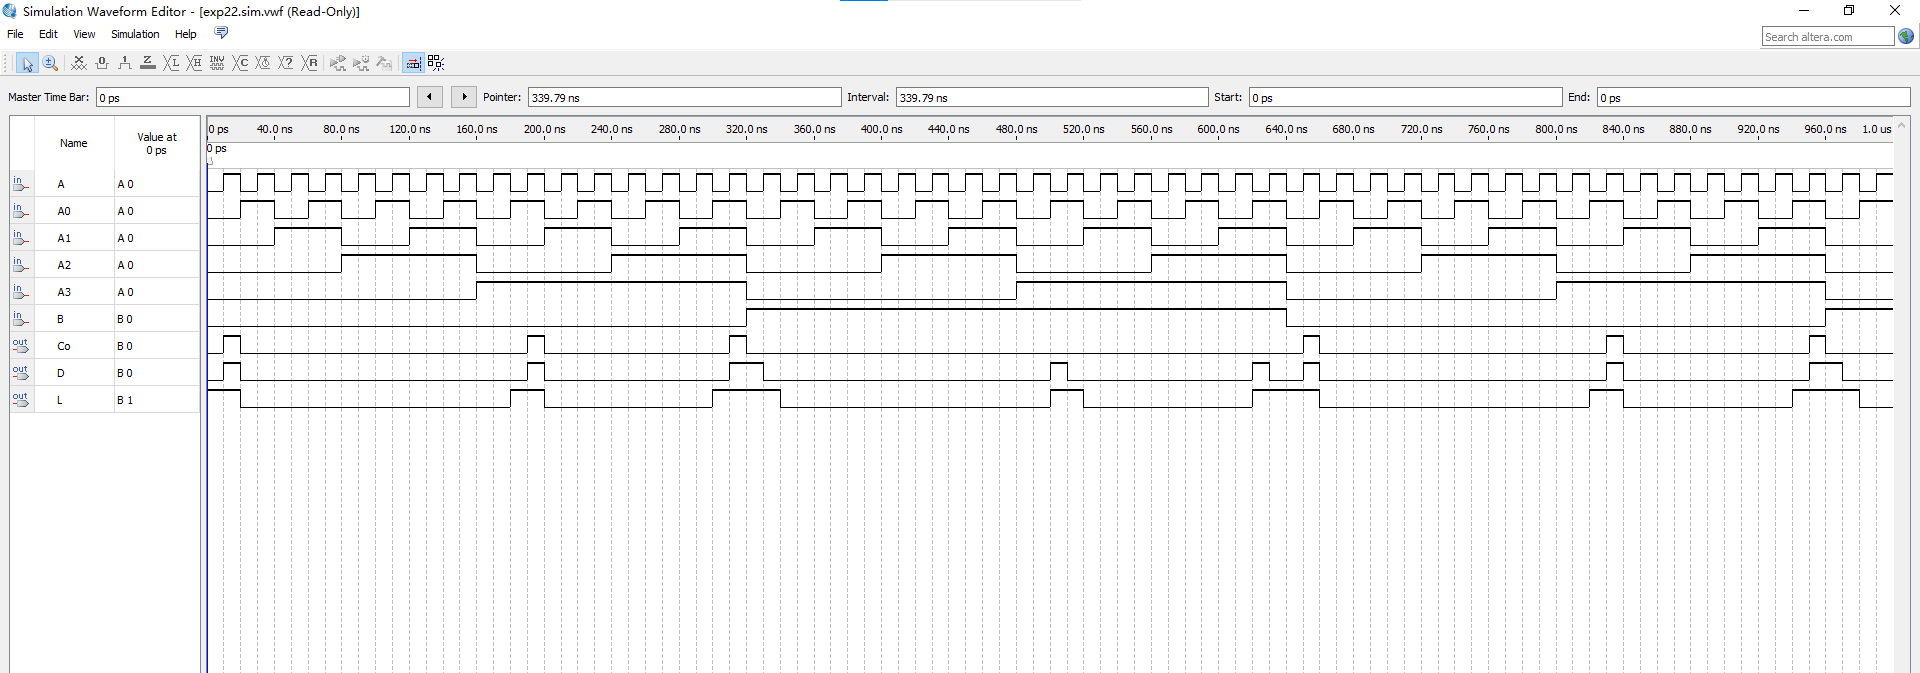
\includegraphics[width=0.75\textwidth]{最终仿真波形.png}
    \caption{密码锁与全减器联动波形仿真结果}
    \label{e2:fig:final_wave}
\end{figure}

由图~\ref{e2:fig:final_wave} 可见，密码输入正确时，全减器输出能够随运算输入变化；密码输入不满足要求时，输出不表示有效运算结果，说明联动控制达到预期。

\subsection{引脚分配与下载验证}

根据实际原理图中的输入、输出端口，在 Quartus II 的 Pin Planner 中完成引脚锁定。由于本实验最终连接同时包含密码输入、全减器输入、密码正确指示和全减器输出，应以当前工程的端口命名和开发板实际接线为准，不在报告中固定列出通用引脚对照表。

完成引脚锁定后重新编译工程，生成可下载文件。连接 USB-Blaster 后，在 Quartus II Programmer 中选择 JTAG 模式并下载至开发板。通过拨动密码输入开关和全减器输入开关，观察对应 LED 状态，验证密码为 \texttt{1111} 时全减器能够正常工作。

\section{实验过程中的问题}

\begin{enumerate}
    \item 在使用 74138 设计密码锁时，需要注意 74138 输出为低有效信号，直接作为密码正确标志可能与 LED 显示或后级控制逻辑的有效电平不一致。因此在原理图连接时，应结合与非门统一信号极性，保证密码正确时控制信号有效。
    \item 在联动全减器和密码锁时，需要明确哪些输入属于密码锁、哪些输入属于全减器，避免仿真激励或引脚分配混淆。最终验证时应先确认密码锁输出正确，再观察全减器差位和借位是否随输入变化。
\end{enumerate}

\section{心得体会}

\begin{enumerate}
    \item 通过本次实验，我进一步理解了 74153 数据选择器和 74138 译码器在组合逻辑设计中的应用。相比直接用基本门电路搭建逻辑函数，中规模集成器件能够使电路结构更清晰，也更便于模块化设计。
    \item 本次实验将全减器和密码锁两个模块连接起来，使我认识到组合逻辑电路不仅要验证单个模块的真值关系，还需要关注模块之间控制信号的极性和有效条件。通过原理图输入、波形仿真和开发板验证，可以较完整地检查设计是否满足实验要求。
\end{enumerate}

% ==================== 实验3：时序电路设计与数码管显示 ====================
\graphicspath{{../3. segment/figures/}}
\chapter{时序电路设计与数码管显示}

\section{实验目的}

\begin{enumerate}
    \item 掌握时序逻辑电路的基本设计方法，理解计数、译码和显示控制之间的关系。
    \item 学习七段数码管显示电路的设计方法，掌握数字编码到段选信号的转换过程。
    \item 掌握利用 Quartus II 进行原理图设计和波形仿真的基本流程。
    \item 能够根据给定数字序列设计显示控制逻辑，并通过仿真波形验证功能正确性。
\end{enumerate}

\section{实验要求}

根据实验要求图片，本实验内容如下：

\begin{enumerate}
    \item 参照参考内容中数码管显示控制电路设计方法，用计数器、七段译码器和若干门电路，用原理图输入方法，在一个 7 段数码管上显示序列：学号（组员 A 学号后 8 位，组员 B 学号后 4 位）。
    \item 用计数器 7490 完成要求 1 中学号循环显示的计数，并显示在数码管中（用一个数码管显示轮次即可）。
\end{enumerate}

要求提交或展示的内容包括：原理图、波形仿真，并下载到 FPGA 验证。

根据补充说明，12 位显示数据选取为\texttt{243025393980}

其中前八位为组员学号后八位 \texttt{24302539}，后四位为另一组员学号后四位 \texttt{3980}。

\section{实验设备}

\begin{itemize}
    \item Quartus II 开发软件
    \item DE0 开发板（FPGA 型号：Cyclone V 5CEBA4F23C7）
    \item USB-Blaster 下载线及计算机
    \item 七段数码管显示模块及相关输入、输出引脚
\end{itemize}

\section{实验原理}

\subsection{时序显示控制}

时序逻辑电路的输出不仅与当前输入有关，还与电路当前状态有关。本实验中，显示控制电路需要依次输出 12 位数字，因此可使用计数器产生当前显示位置，再由组合逻辑根据计数状态选择对应数字。计数状态循环变化时，显示内容也随之按预定序列循环输出。

若计数器当前状态记为 $Q$，待显示数字记为 $D$，则显示控制可表示为
\[
    D = f(Q).
\]
其中 $f(Q)$ 按照实验要求依次给出 \texttt{2,4,3,0,2,5,3,9,3,9,8,0}。当计数器完成 12 个状态后回到初始状态，即可实现 12 位数字的循环显示。

\subsection{七段数码管译码}

七段数码管由 $a,b,c,d,e,f,g$ 七个发光段组成。不同数字对应不同段选组合，译码电路根据输入的 BCD 码产生相应段选信号。以共阴极、段选高电平有效为例，常用数字与七段码关系如表~\ref{e3:tab:segment_code} 所示。

\begin{table}[H]
    \centering
    \caption{十进制数字与七段显示关系}
    \label{e3:tab:segment_code}
    \begin{tabular}{c c c}
        \toprule
        \textbf{十进制数字} & \textbf{BCD 码} & \textbf{点亮段} \\
        \midrule
        0 & 0000 & $a,b,c,d,e,f$ \\
        1 & 0001 & $b,c$ \\
        2 & 0010 & $a,b,d,e,g$ \\
        3 & 0011 & $a,b,c,d,g$ \\
        4 & 0100 & $b,c,f,g$ \\
        5 & 0101 & $a,c,d,f,g$ \\
        6 & 0110 & $a,c,d,e,f,g$ \\
        7 & 0111 & $a,b,c$ \\
        8 & 1000 & $a,b,c,d,e,f,g$ \\
        9 & 1001 & $a,b,c,d,f,g$ \\
        \bottomrule
    \end{tabular}
\end{table}

实际实验中若数码管为低电平有效，只需在输出端对段选信号取反。通过计数器、数据选择逻辑和七段译码逻辑的配合，即可将给定数字序列转换为数码管上可观察的显示结果。

\section{实验内容}

\subsection{新建工程}

打开 Quartus II，选择 \textbf{File $\rightarrow$ New Project Wizard} 新建实验三工程。工程目录选择实验三文件夹，顶层实体名与原理图文件名保持一致。器件选择 DE0 开发板对应的 Cyclone V \texttt{5CEBA4F23C7}。工程建立完成后，选择 \textbf{File $\rightarrow$ New $\rightarrow$ Block Diagram/Schematic File} 新建原理图文件，并保存为顶层设计文件。

\subsection{放置实验元件}

在原理图编辑界面中打开元件库，依次放置本实验需要的器件：计数器、7447 七段译码器、若干基本门电路、输入引脚和输出引脚。输入引脚用于连接时钟和复位信号，输出引脚用于连接七段数码管的段选信号。放置元件时先把计数器放在左侧，7447 放在右侧，中间留出位置连接门电路，便于后续检查连线。

\subsection{确定显示顺序}

本组需要显示的序列为 \texttt{243025393980}。在设计原理图前，先把 12 个数字按显示顺序列出，如表~\ref{e3:tab:display_sequence} 所示。

\begin{table}[H]
    \centering
    \caption{显示状态与数字序列对应关系}
    \label{e3:tab:display_sequence}
    \begin{tabular}{ccccccccccccc}
        \toprule
        \textbf{轮次} & 0 & 1 & 2 & 3 & 4 & 5 & 6 & 7 & 8 & 9 & 10 & 11 \\
        \midrule
        \textbf{显示数字} & 2 & 4 & 3 & 0 & 2 & 5 & 3 & 9 & 3 & 9 & 8 & 0 \\
        \bottomrule
    \end{tabular}
\end{table}

原理图连线时，使计数器输出依次代表表中的轮次。每来一个时钟脉冲，轮次前进一位；显示到第 11 位后，下一次重新回到第 0 位。

\subsection{连接计数器}

将时钟输入端接到计数器的时钟端，将复位输入端接到计数器的清零端。计数器输出端作为当前显示轮次信号，连接到后级门电路。为了只显示 12 个轮次，需要在计数到序列末尾后产生复位信号，使计数器重新从 0 开始。

完成计数器部分后，先检查时钟端、清零端和输出端是否全部连接，避免出现输入悬空或输出未接入后级逻辑的问题。

\subsection{连接序列选择逻辑}

根据表~\ref{e3:tab:display_sequence}，把每一个轮次对应到一个显示数字，并把该数字转换为 4 位 BCD 码后送入 7447。实际连线时，先确定 7447 的四个输入端，再分别用门电路连接出这四路 BCD 信号。

例如，轮次 0 对应数字 2，送入 7447 的 BCD 码为 \texttt{0010}；轮次 1 对应数字 4，BCD 码为 \texttt{0100}；轮次 2 对应数字 3，BCD 码为 \texttt{0011}；轮次 3 对应数字 0，BCD 码为 \texttt{0000}。其余轮次也按同样方法连接。完成后，从计数器输出到 7447 输入之间应形成完整的序列选择电路。

\subsection{连接 7447 与数码管输出}

将序列选择逻辑输出的 4 位 BCD 信号接入 7447 的输入端。再将 7447 的输出端分别连接到七段数码管的 $a,b,c,d,e,f,g$ 段选输出引脚。连线时按段名逐一对应，不交换段选顺序。

由于实验要求只用一个数码管显示轮次，因此只保留一个数码管参与显示。若原理图中有多个数码管相关输出，只使用本实验对应的一个数码管输出，其余无关显示位不参与本次验证。

\subsection{编译原理图}

原理图连接完成后，保存文件并设置为顶层实体。点击 \textbf{Start Compilation} 进行编译。若出现报错，按提示检查元件引脚是否漏接、线名是否重复、输入输出方向是否设置错误。确认没有错误后，得到完整的仿真电路图，如图~\ref{e3:fig:circuit} 所示。

\begin{figure}[htbp]
    \centering
    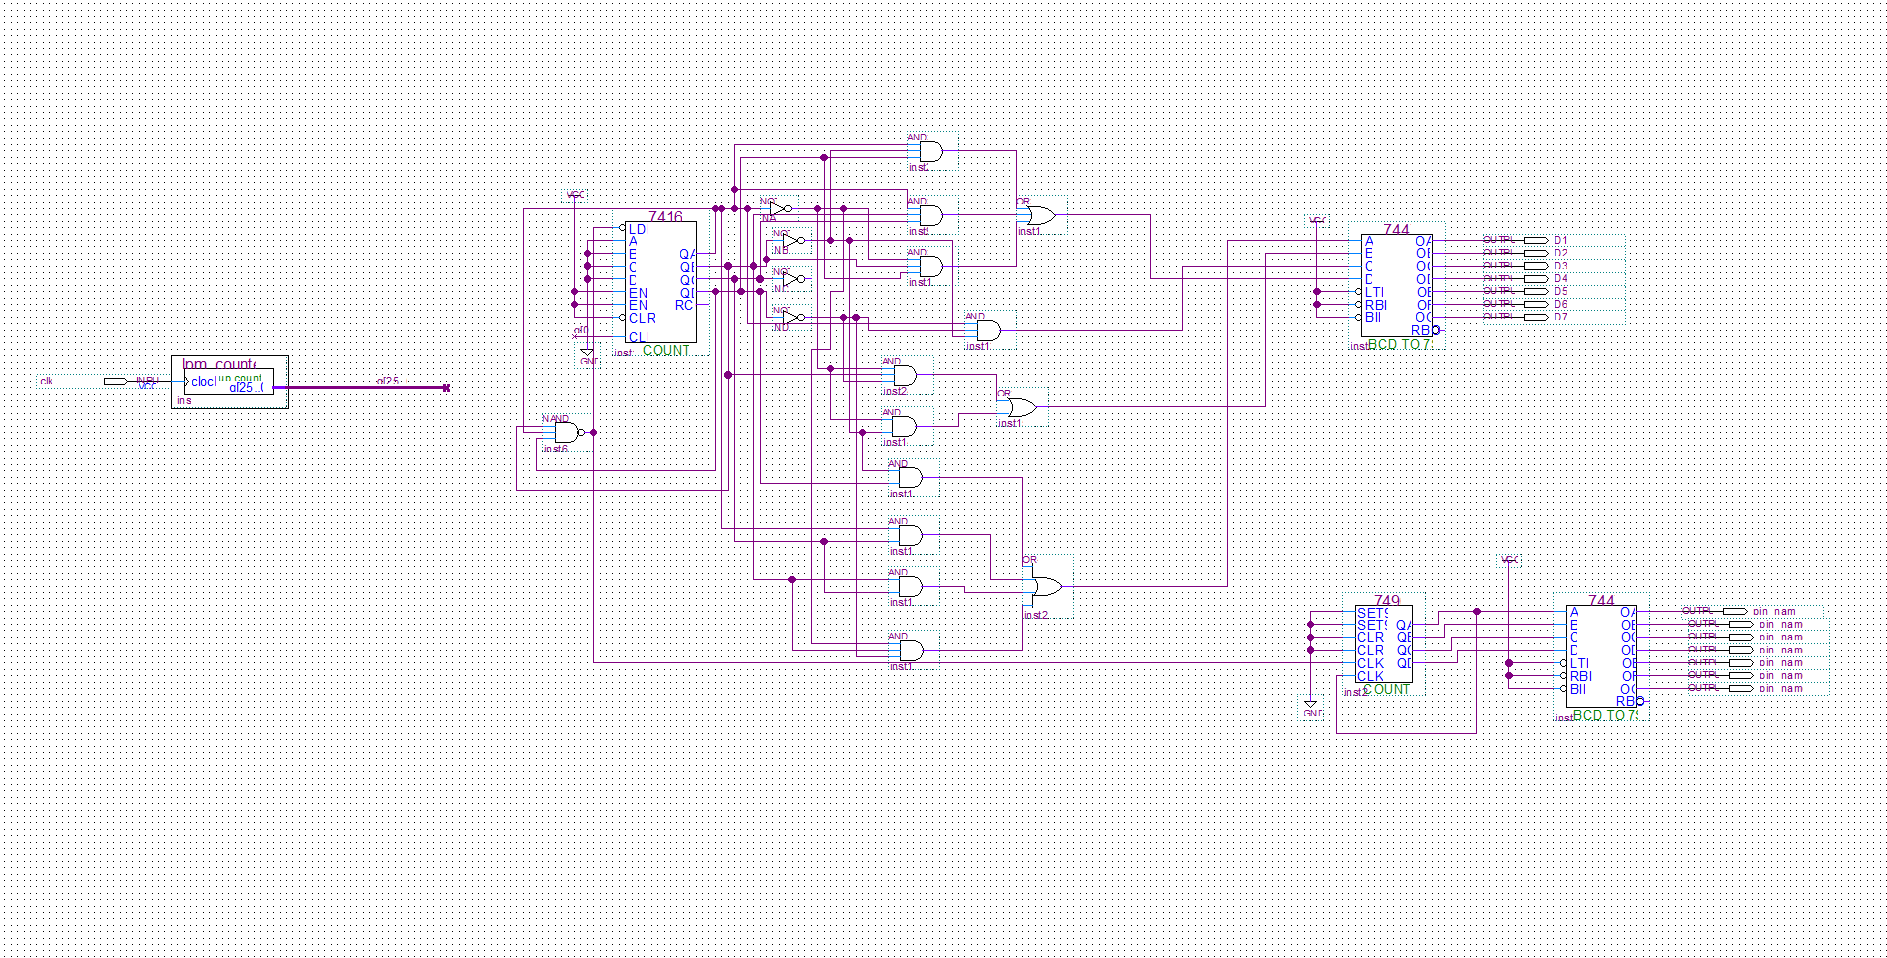
\includegraphics[width=0.75\textwidth]{仿真电路图.png}
    \caption{仿真电路图}
    \label{e3:fig:circuit}
\end{figure}

\subsection{建立波形仿真文件}

选择 \textbf{File $\rightarrow$ New $\rightarrow$ Verification/Debugging $\rightarrow$ Vector Waveform File} 新建波形文件。通过 \textbf{Insert Node or Bus} 加入时钟、复位、计数器输出、7447 输入和七段输出信号。设置时钟信号周期，并在仿真开始时给复位端一个有效脉冲，使电路从第 0 轮开始显示。

运行仿真后，按顺序检查计数器输出和 7447 输入：轮次应依次变化，7447 输入应对应 \texttt{2,4,3,0,2,5,3,9,3,9,8,0}。再观察七段输出，确认每一轮对应的数码管显示数字正确。仿真结果如图~\ref{e3:fig:wave} 所示。

\begin{figure}[htbp]
    \centering
    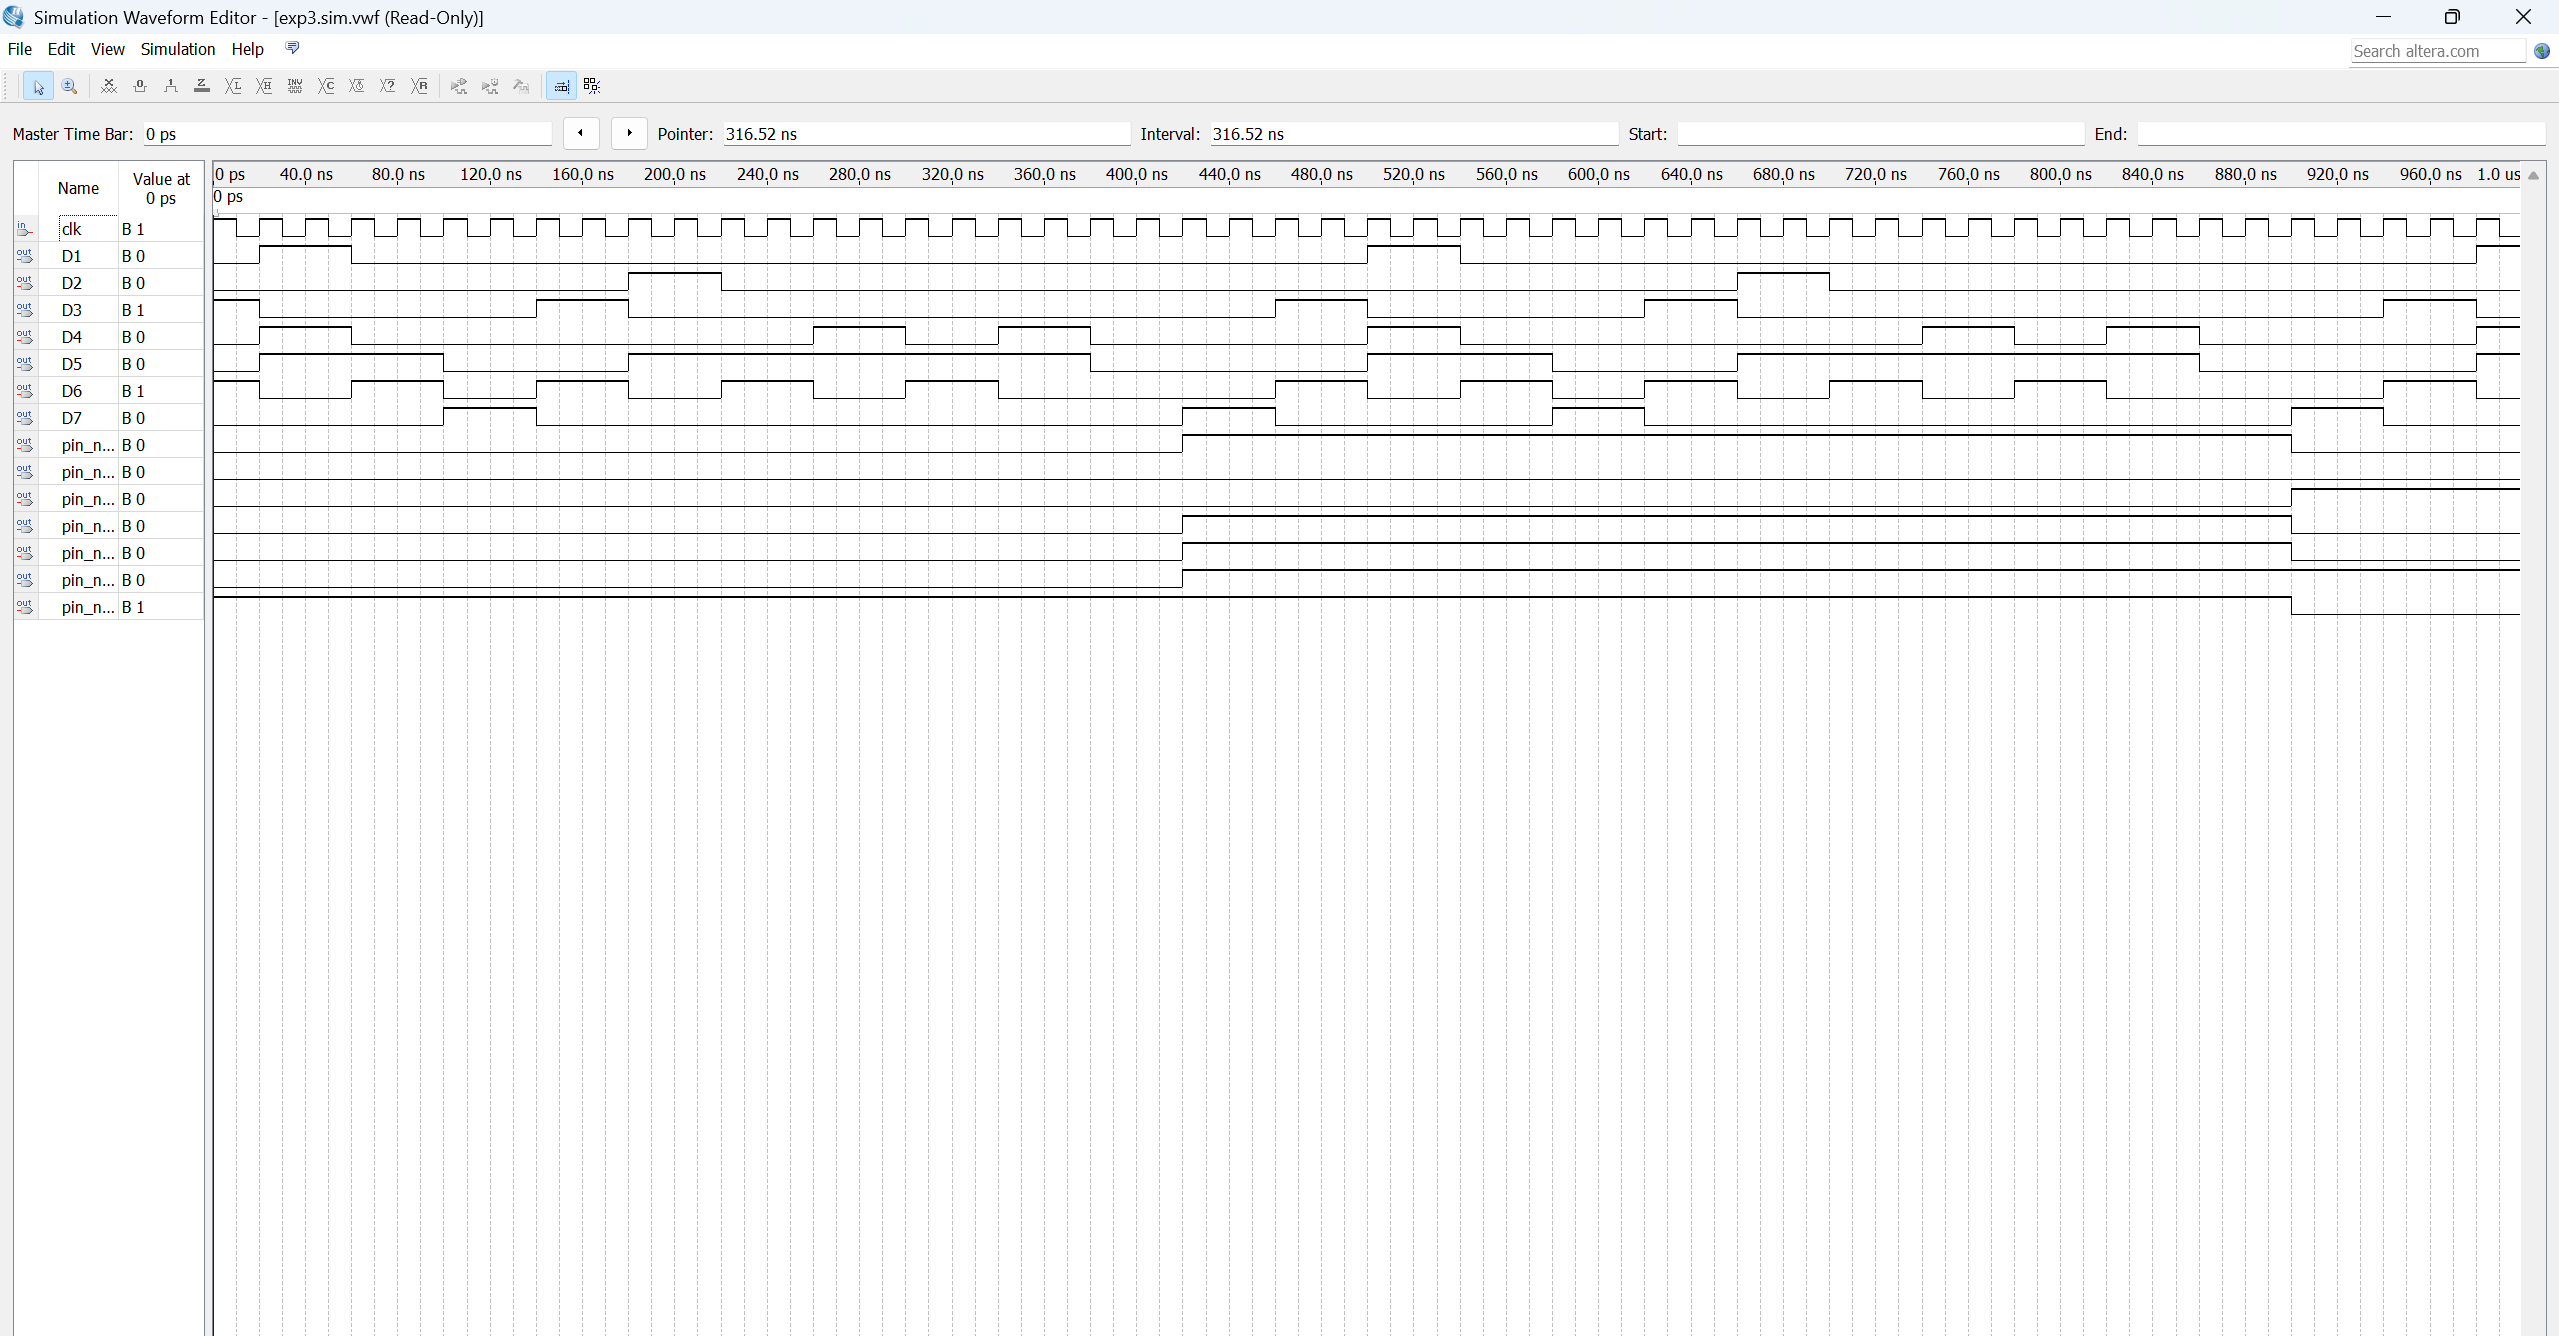
\includegraphics[width=0.75\textwidth]{仿真波形图.png}
    \caption{仿真波形图}
    \label{e3:fig:wave}
\end{figure}

\subsection{下载到 FPGA 验证}

仿真确认无误后，打开 Pin Planner，将时钟、复位和七段数码管输出分配到 DE0 开发板对应引脚。引脚分配完成后重新编译工程。随后连接 USB-Blaster，打开 Programmer，选择 JTAG 模式，加载生成的 \texttt{.sof} 文件并点击 \textbf{Start} 下载。

下载完成后，在开发板上观察 7 段数码管显示。按时钟输入变化时，数码管应按照 \texttt{243025393980} 的顺序循环显示。若显示顺序不对，返回检查计数器复位和序列选择逻辑；若数字笔段不对，返回检查 7447 输出与数码管段选引脚的对应关系。

\section{实验过程中的问题}

\begin{enumerate}
    \item 在设计显示电路时，需要区分 BCD 数字编码和七段数码管段选信号。若将二者直接混用，仿真中可能出现数字状态正确但数码管显示错误的问题，因此应先确定数字编码，再统一进行七段译码。
    \item 七段数码管存在高电平有效和低电平有效两种连接方式。仿真和实际下载验证时，应根据器件连接方式判断是否需要对段选信号取反，避免显示结果与预期数字相反或部分笔段异常点亮。
    \item 本实验目录中未提供 Verilog 源码或 Quartus 工程文件，因此报告主要依据实验说明和现有仿真截图整理，不额外列出代码清单。
\end{enumerate}

\section{心得体会}

\begin{enumerate}
    \item 通过本次实验，我进一步理解了时序逻辑电路和组合译码电路的配合方式。计数器负责产生状态，组合逻辑负责根据状态选择显示数字，七段译码器则把抽象数字转换为具体显示信号。
    \item 本次实验说明，数码管显示电路的关键不仅是写出数字序列，还要正确处理状态循环、编码转换和有效电平。通过观察仿真波形，可以较直观地检查显示顺序和段选输出是否符合设计要求。
\end{enumerate}

% ==================== 实验4：基于硬件描述语言电路设计 ====================
\graphicspath{{../4. fpga/figures/}}
\chapter{基于硬件描述语言电路设计}

\section{实验目的}

\begin{enumerate}
    \item 掌握 VHDL 硬件描述语言的基本语法，理解实体（Entity）、结构体（Architecture）、信号（Signal）和进程（Process）等核心概念。
    \item 学习使用 VHDL 分别设计组合逻辑电路（异或门、七段码译码器）和时序逻辑电路（计数器、分频器），并在 Quartus II 中进行编译和波形仿真验证。
    \item 掌握 Quartus II 中 VHDL 文件的编译、生成原理图模块符号（Create Symbol Files）以及在顶层原理图中调用 VHDL 模块的基本流程。
    \item 能够将多个独立设计的 VHDL 模块在顶层原理图中组合连接，实现较复杂的数字系统设计，并下载到 DE0 开发板进行硬件验证。
\end{enumerate}

\section{实验要求}

\begin{enumerate}
    \item \textbf{要求 1}：学习并掌握硬件描述语言 VHDL，熟悉门电路的逻辑功能，并用硬件描述语言实现门电路的设计。参考"参考内容 1"中给出的与门源程序，编写一个异或门逻辑电路。用 Quartus II 波形仿真验证，下载到 DE0 开发板验证。
    \item \textbf{要求 2}：熟悉中规模器件译码器的逻辑功能，用硬件描述语言实现其设计。参考"参考内容 2"中给出的将 8421BCD 码转换成 0--9 的七段码译码器源程序，编写一个将二进制码转换成 0--E 的七段码译码器。用 Quartus II 波形仿真验证，下载到 DE0 开发板，利用开发板上的数码管验证。
    \item \textbf{要求 3}：熟悉时序电路计数器的逻辑功能，用硬件描述语言实现其设计。参考"参考内容 3"中给出的四位二进制计数器的源程序，编写一个计数器实现 0--E 计数。用 Quartus II 波形仿真验证。
    \item \textbf{要求 4}：熟悉分频电路的逻辑功能，并用硬件描述语言实现其设计。参考"参考内容 4"中给出的 50M 分频器的源程序，编写一个能实现占空比 50\% 的 5M 和 50M 分频器即两个输出，输出信号频率分别为 10Hz 和 1Hz。下载到 DE0 开发板验证（提示：利用 DE0 板上已有的 50M 晶振作为输入信号，通过开发板上两个的 LED 灯观察输出信号）。
    \item \textbf{要求 5}：利用已经实现的 VHDL 模块文件，顶层文件采用原理图设计方法，实现 A 学号后 4 位（3980）、F,E,E,L、学号后 4 位（0938）共 12 位字符在七段数码管上自动循环显示，频率 1Hz 和 10Hz 可以自动切换（提示：如何将 VHDL 模块文件在顶层原理图文件中引用，参考参考内容 5）。
\end{enumerate}

\section{实验设备}

\begin{itemize}
    \item Quartus II 开发软件
    \item DE0 开发板（FPGA 型号：Cyclone V 5CEBA4F23C7）
    \item USB-Blaster 下载线及计算机
    \item 七段数码管显示模块及相关输入、输出引脚
\end{itemize}

\section{实验原理}

\subsection{VHDL 基本结构}

VHDL（Very High Speed Integrated Circuit Hardware Description Language）是一种用于描述数字电路行为和结构的硬件描述语言。一个完整的 VHDL 设计文件由三部分组成：

\begin{enumerate}
    \item \textbf{库引用}：通过 \texttt{library} 和 \texttt{use} 语句引入标准库。\texttt{ieee.std\_logic\_1164.all} 提供 \texttt{std\_logic} 和 \texttt{std\_logic\_vector} 等标准逻辑类型；\texttt{ieee.numeric\_std.all} 提供 \texttt{unsigned}、\texttt{signed} 等数值类型及算术运算支持。
    \item \textbf{实体（Entity）}：定义模块的外部接口，通过 \texttt{port()} 声明输入输出端口。端口类型包括 \texttt{std\_logic}（单比特信号）和 \texttt{std\_logic\_vector}（多比特总线），方向有 \texttt{in}、\texttt{out}、\texttt{inout} 和 \texttt{buffer}。
    \item \textbf{结构体（Architecture）}：描述模块的内部行为或结构。可使用并发信号赋值语句实现组合逻辑，或使用 \texttt{process} 进程块实现时序逻辑。
\end{enumerate}

\subsection{组合逻辑设计}

组合逻辑电路的输出仅取决于当前输入，无记忆功能。在 VHDL 中，组合逻辑可通过以下两种方式实现：

\begin{itemize}
    \item \textbf{并发信号赋值}：直接在结构体中使用赋值语句，如 \texttt{C <= A xor B;}，描述异或门逻辑。
    \item \textbf{进程中的 \texttt{case} 语句}：在 \texttt{process} 块中使用 \texttt{case} 语句进行多路选择，适用于译码器等多输入多输出的组合逻辑。
\end{itemize}

七段码译码器是典型的组合逻辑电路：根据 4 位 BCD 输入，通过 \texttt{case} 语句选择对应的 7 位段选码输出。DE0 开发板的七段数码管为共阳极结构，段选信号低电平有效（0 表示点亮，1 表示熄灭）。各数字对应的段选编码如表~\ref{e4:tab:hex_decode} 所示。

\begin{table}[H]
    \centering
    \caption{8421BCD 转七段码译码真值表}
    \label{e4:tab:hex_decode}
    \begin{tabular}{cccc}
        \toprule
        \textbf{BCD 输入} & \textbf{十六进制} & \textbf{seg\_out[6:0]} & \textbf{显示字符} \\
        \midrule
        0000 & 0 & 1000000 & 0 \\
        0001 & 1 & 1111001 & 1 \\
        0010 & 2 & 0100100 & 2 \\
        0011 & 3 & 0110000 & 3 \\
        0100 & 4 & 0011001 & 4 \\
        0101 & 5 & 0010010 & 5 \\
        0110 & 6 & 0000010 & 6 \\
        0111 & 7 & 1111000 & 7 \\
        1000 & 8 & 0000000 & 8 \\
        1001 & 9 & 0010000 & 9 \\
        1010 & A & 0001000 & A \\
        1011 & b & 0000011 & b \\
        1100 & C & 1000110 & C \\
        1101 & d & 0100001 & d \\
        1110 & E & 0000110 & E \\
        1111 & -- & 1111111 & 灭灯 \\
        \bottomrule
    \end{tabular}
\end{table}

\subsection{时序逻辑设计}

时序逻辑电路的输出不仅与当前输入有关，还与电路的历史状态有关，依赖时钟信号驱动状态变化。在 VHDL 中，时序逻辑通过 \texttt{process(clk, rst)} 进程块实现，使用 \texttt{rising\_edge(clk)} 检测时钟上升沿来触发寄存器更新。

模 $N$ 计数器是最基本的时序逻辑电路之一。以模 15 计数器为例，每个时钟上升沿计数值加 1，当计数到 14（即十六进制 E）后，下一个时钟回到 0，同时产生一个时钟周期宽度的进位脉冲 COUT。计数器还具有异步清零功能：当复位信号 \texttt{rst} 为低电平时，计数值立即清零。

\subsection{分频器原理}

分频器通过对高频时钟信号进行计数来产生低频输出信号。若输入时钟频率为 $f_{\text{clk}}$，期望输出频率为 $f_{\text{out}}$，则需要的半周期计数值为
\[
    N = \frac{f_{\text{clk}}}{2 \times f_{\text{out}}}
\]
计数器每计满 $N$ 次，将输出信号翻转一次，即可产生占空比 50\% 的方波。

对于 DE0 开发板上 50MHz 的晶振时钟：
\begin{itemize}
    \item 分频到 1Hz：$N = 50{,}000{,}000 / 2 = 25{,}000{,}000$
    \item 分频到 10Hz：$N = 50{,}000{,}000 / (2 \times 10) = 2{,}500{,}000$
\end{itemize}

\subsection{综合设计原理}

要求 5 的综合设计需要将计数器、译码器和分频/速度切换模块组合，实现 12 位字符的循环显示，并在 1Hz 和 10Hz 之间自动切换速度。

显示序列为 \texttt{2539FEEL3980}，由三部分组成：组员 B 学号后 4 位（2539）、固定字符 F,E,E,L、以及组员 A 学号后 4 位（3980）。M12 计数器从 0 计数到 11，每个计数值通过特殊七段码译码器映射到对应的显示字符，如表~\ref{e4:tab:display_map} 所示。

\begin{table}[H]
    \centering
    \caption{综合设计显示序列映射表}
    \label{e4:tab:display_map}
    \begin{tabular}{cccc}
        \toprule
        \textbf{计数值} & \textbf{BCD 码} & \textbf{显示字符} & \textbf{SG\_OUT[6:0]} \\
        \midrule
        0  & 0000 & 2 & 0100100 \\
        1  & 0001 & 5 & 0010010 \\
        2  & 0010 & 3 & 0110000 \\
        3  & 0011 & 9 & 0010000 \\
        4  & 0100 & F & 0001110 \\
        5  & 0101 & E & 0000110 \\
        6  & 0110 & E & 0000110 \\
        7  & 0111 & L & 1000111 \\
        8  & 1000 & 3 & 0110000 \\
        9  & 1001 & 9 & 0010000 \\
        10 & 1010 & 8 & 0000000 \\
        11 & 1011 & 0 & 1000000 \\
        \bottomrule
    \end{tabular}
\end{table}

综合设计由三个核心模块组成：

\begin{enumerate}
    \item \textbf{M12 计数器}（\texttt{exa4\_3\_2}）：0 到 11 循环计数，带使能信号 \texttt{en}，仅在 \texttt{en=1} 时计数加 1。计数到 11 后回到 0，同时输出一个 \texttt{cout} 脉冲，表示一轮显示结束。
    \item \textbf{特殊七段码译码器}（\texttt{exa4\_2\_2}）：根据 M12 计数器的当前值，输出对应字符的七段码。
    \item \textbf{自动切换控制器}（\texttt{exa4\_auto\_1hz\_10hz}）：内部集成 1Hz 和 10Hz 两种分频模式。每当 M12 计数器完成一轮显示（\texttt{cout=1}），自动切换到另一种速度。其 \texttt{tick} 输出作为 M12 计数器的使能输入，形成闭环控制。
\end{enumerate}

顶层原理图中三个模块的连接关系为：50MHz 时钟同时连接到自动切换控制器和 M12 计数器的时钟端；复位信号同时连接到两者的复位端；自动切换控制器的 \texttt{tick} 输出连接到 M12 计数器的 \texttt{en} 输入；M12 计数器的 \texttt{dout} 连接到译码器的 \texttt{BCD\_IN}；M12 计数器的 \texttt{cout} 反馈连接到自动切换控制器的 \texttt{loop\_end} 输入；译码器的 \texttt{SG\_OUT} 输出连接到 HEX0 数码管引脚。

\section{实验内容}

\subsection{要求 1：异或门电路}

\subsubsection{创建工程与编写 VHDL}

打开 Quartus II，选择 \textbf{File $\rightarrow$ New Project Wizard} 新建工程。器件选择 DE0 开发板对应的 Cyclone V \texttt{5CEBA4F23C7}。选择 \textbf{File $\rightarrow$ New $\rightarrow$ VHDL File} 新建 VHDL 文件，输入异或门源码并保存为 \texttt{exa4\_1\_xor.vhd}。

\begin{minted}{vhdl}
library ieee;
use ieee.std_logic_1164.all;

entity exa4_1_xor is
port(
    A : in  std_logic;
    B : in  std_logic;
    C : out std_logic
);
end exa4_1_xor;

architecture rtl of exa4_1_xor is
begin
    C <= A xor B;
end rtl;
\end{minted}
\captionof{listing}{异或门 VHDL 源码（exa4\_1\_xor.vhd）}
\label{e4:lst:xor}

该设计定义了一个具有两个输入端 A、B 和一个输出端 C 的异或门，结构体中使用并发信号赋值语句直接描述异或逻辑。

\subsubsection{编译与生成原理图框图}

点击 \textbf{Start Compilation} 对 VHDL 文件进行完整编译。编译通过后，选择 \textbf{File $\rightarrow$ Create/Update $\rightarrow$ Create Symbol Files for Current File}，将 VHDL 模块生成可在原理图中调用的模块符号文件（\texttt{.bsf}）。

\subsubsection{建立顶层原理图}

选择 \textbf{File $\rightarrow$ New $\rightarrow$ Block Diagram/Schematic File} 新建原理图文件。在元件库的 Project 目录下找到刚生成的 \texttt{exa4\_1\_xor} 符号并放置到原理图中，然后添加输入引脚 A、B 和输出引脚 C，完成连线。顶层原理图如图~\ref{e4:fig:task1_circuit} 所示。

\begin{figure}[htbp]
    \centering
    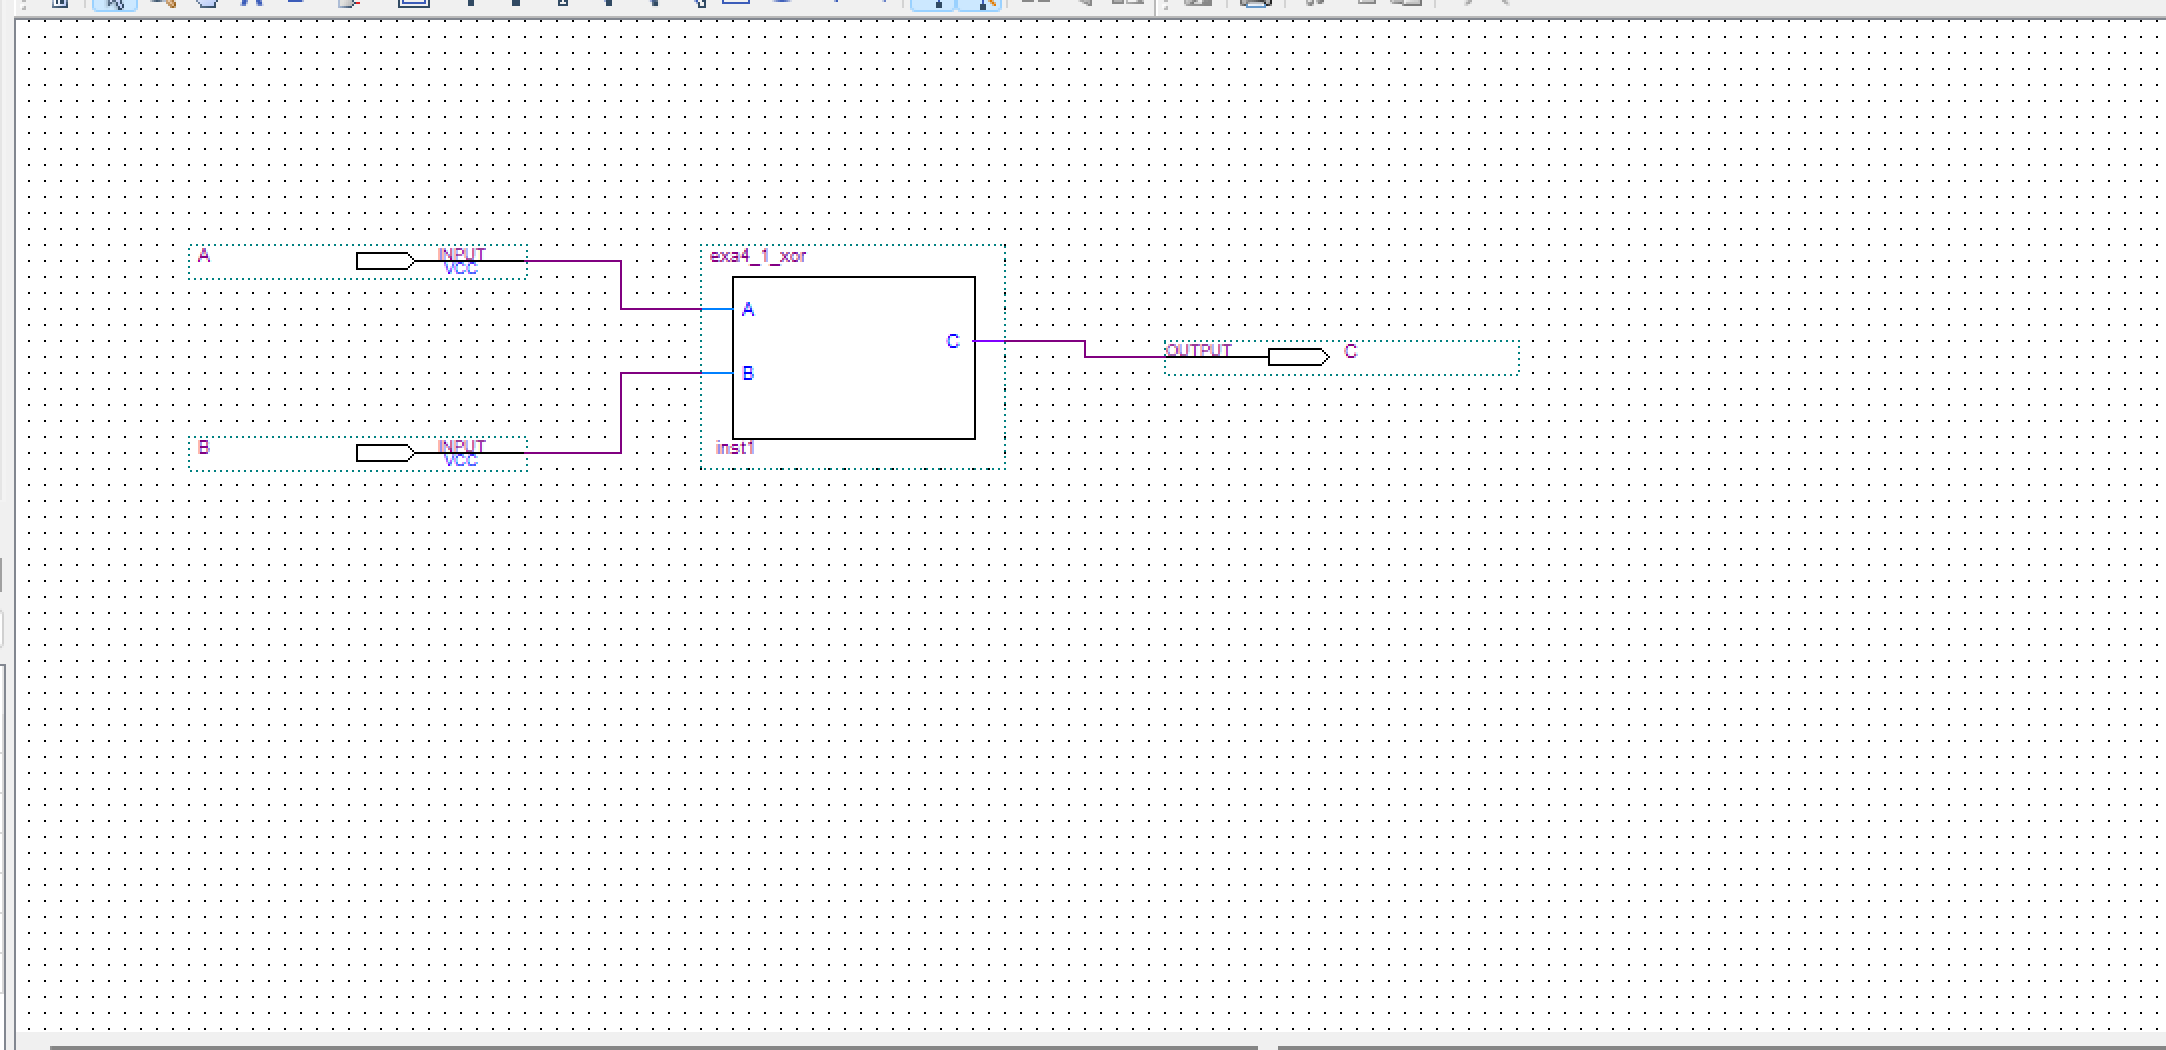
\includegraphics[width=0.75\textwidth]{要求1电路.png}
    \caption{要求 1 异或门 BDF 原理图}
    \label{e4:fig:task1_circuit}
\end{figure}

\subsubsection{波形仿真验证}

将原理图文件设置为顶层实体并重新编译。选择 \textbf{File $\rightarrow$ New $\rightarrow$ Vector Waveform File} 新建波形文件，加入 A、B、C 三个信号。设置 A 的周期为 20ns、B 的周期为 40ns，运行功能仿真。仿真结果如图~\ref{e4:fig:task1_sim} 所示。

\begin{figure}[htbp]
    \centering
    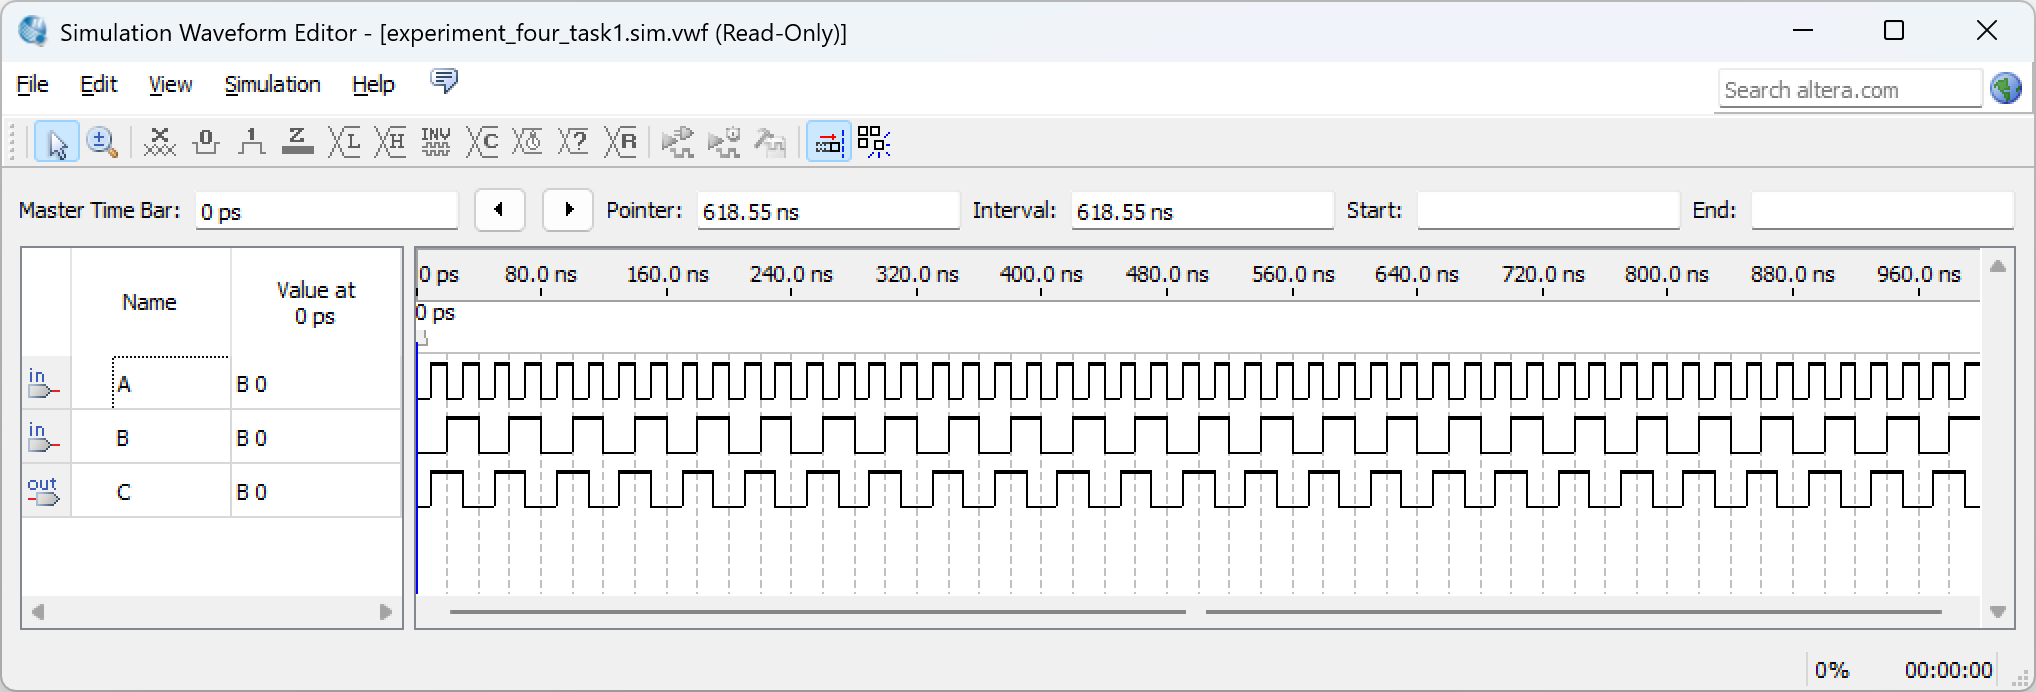
\includegraphics[width=0.75\textwidth]{要求1仿真.png}
    \caption{要求 1 异或门仿真波形}
    \label{e4:fig:task1_sim}
\end{figure}

从仿真波形可以看出，当 A 和 B 的输入电平相同时，输出 C 为低电平；当 A 和 B 的输入电平不同时，输出 C 为高电平，符合异或门的逻辑功能。

\subsubsection{引脚分配与下载验证}

打开 Pin Planner，将输入 A、B 分别分配到开发板的拨动开关 SW0（PIN\_U13）和 SW1（PIN\_V13），输出 C 分配到 LEDR0（PIN\_AA2）。重新编译工程后，连接 USB-Blaster，选择 JTAG 模式下载 \texttt{.sof} 文件到 FPGA。在开发板上拨动开关，观察 LED 指示灯正确反映异或逻辑。

\subsection{要求 2：8421BCD 转七段码译码器}

\subsubsection{创建工程与编写 VHDL}

新建 Quartus II 工程，创建 VHDL 文件 \texttt{exa4\_2\_hex\_0e.vhd}，编写支持 0--E 共 15 个字符显示的七段码译码器。

\begin{minted}{vhdl}
library ieee;
use ieee.std_logic_1164.all;

entity exa4_2_hex_0e is
port(
    data_in : in  std_logic_vector(3 downto 0);
    seg_out : out std_logic_vector(6 downto 0)
);
end exa4_2_hex_0e;

architecture rtl of exa4_2_hex_0e is
begin
    process(data_in)
    begin
        case data_in is
            when "0000" => seg_out <= "1000000"; -- 0
            when "0001" => seg_out <= "1111001"; -- 1
            when "0010" => seg_out <= "0100100"; -- 2
            when "0011" => seg_out <= "0110000"; -- 3
            when "0100" => seg_out <= "0011001"; -- 4
            when "0101" => seg_out <= "0010010"; -- 5
            when "0110" => seg_out <= "0000010"; -- 6
            when "0111" => seg_out <= "1111000"; -- 7
            when "1000" => seg_out <= "0000000"; -- 8
            when "1001" => seg_out <= "0010000"; -- 9
            when "1010" => seg_out <= "0001000"; -- A
            when "1011" => seg_out <= "0000011"; -- b
            when "1100" => seg_out <= "1000110"; -- C
            when "1101" => seg_out <= "0100001"; -- d
            when "1110" => seg_out <= "0000110"; -- E
            when others => seg_out <= "1111111"; -- blank
        end case;
    end process;
end rtl;
\end{minted}
\captionof{listing}{七段码译码器 VHDL 源码（exa4\_2\_hex\_0e.vhd）}
\label{e4:lst:hex}

该译码器将 4 位 BCD 输入转换为 7 位段选信号输出。\texttt{process} 的敏感列表为 \texttt{data\_in}，当输入变化时自动重新计算输出，实现纯组合逻辑行为。段选码已按共阳极低电平有效编码，可直接驱动 DE0 开发板的七段数码管。

\subsubsection{编译、生成原理图框图与建立顶层原理图}

编译 VHDL 文件后生成模块符号。新建 BDF 原理图，放置 \texttt{exa4\_2\_hex\_0e} 符号，添加 4 位输入总线 \texttt{data\_in[3..0]} 和 7 位输出总线 \texttt{seg\_out[6..0]}，完成连线。顶层原理图如图~\ref{e4:fig:task2_circuit} 所示。

\begin{figure}[htbp]
    \centering
    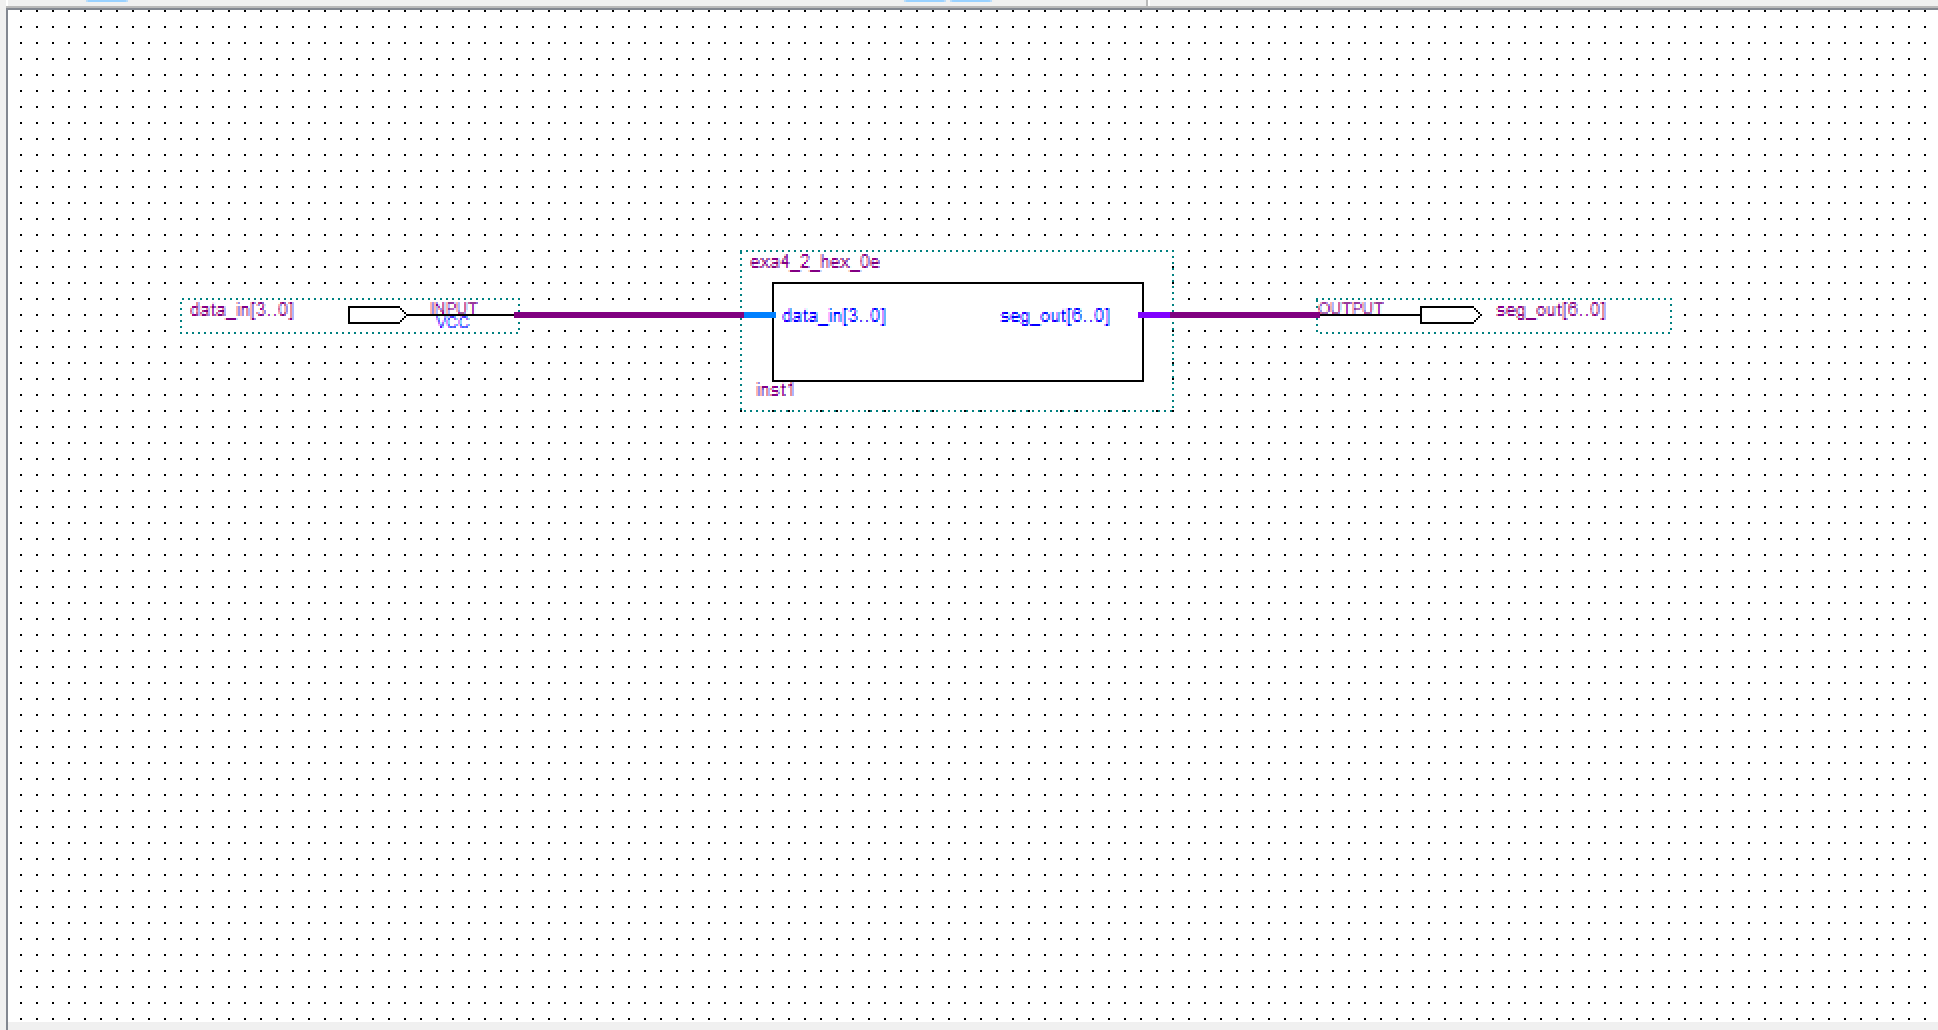
\includegraphics[width=0.75\textwidth]{要求2电路.png}
    \caption{要求 2 七段码译码器 BDF 原理图}
    \label{e4:fig:task2_circuit}
\end{figure}

\subsubsection{波形仿真验证}

建立波形文件，设置 \texttt{data\_in} 依次从 0000 变化到 1111，每个输入保持一定时间。运行仿真后，检查 \texttt{seg\_out} 的输出是否与表~\ref{e4:tab:hex_decode} 中的真值表一致。仿真结果表明，16 种输入组合的段选输出均正确。

\subsubsection{引脚分配与下载验证}

将 \texttt{data\_in[3:0]} 分配到拨动开关 SW3--SW0（PIN\_T12、PIN\_T13、PIN\_V13、PIN\_U13），\texttt{seg\_out[6:0]} 分配到 HEX0 数码管的 7 个段选引脚（PIN\_AA22、PIN\_Y21、PIN\_Y22、PIN\_W21、PIN\_W22、PIN\_V21、PIN\_U21）。重新编译并下载到 FPGA 后，拨动开关选择不同的 BCD 码，观察数码管正确显示 0--E 各字符。

\subsection{要求 3：模 15 计数器}

\subsubsection{创建工程与编写 VHDL}

新建工程，创建 VHDL 文件 \texttt{exa4\_3\_counter\_0e.vhd}，编写模 15 计数器。

\begin{minted}{vhdl}
library ieee;
use ieee.std_logic_1164.all;
use ieee.numeric_std.all;

entity exa4_3_counter_0e is
port(
    clk  : in  std_logic;
    rst  : in  std_logic;
    DOUT : out std_logic_vector(3 downto 0);
    COUT : out std_logic
);
end exa4_3_counter_0e;

architecture rtl of exa4_3_counter_0e is
    signal count_q : unsigned(3 downto 0) := (others => '0');
    signal cout_q  : std_logic := '0';
begin
    process(clk, rst)
    begin
        if rst = '0' then
            count_q <= (others => '0');
            cout_q <= '0';
        elsif rising_edge(clk) then
            if count_q = to_unsigned(14, 4) then
                count_q <= (others => '0');
                cout_q <= '1';
            else
                count_q <= count_q + 1;
                cout_q <= '0';
            end if;
        end if;
    end process;

    DOUT <= std_logic_vector(count_q);
    COUT <= cout_q;
end rtl;
\end{minted}
\captionof{listing}{模 15 计数器 VHDL 源码（exa4\_3\_counter\_0e.vhd）}
\label{e4:lst:counter}

该计数器使用 \texttt{ieee.numeric\_std} 库的 \texttt{unsigned} 类型进行计数，支持异步低电平复位。每个时钟上升沿计数加 1，当计数到 14 时下一个时钟回到 0 并产生一个周期的进位脉冲 COUT。

\subsubsection{编译、生成原理图框图与建立顶层原理图}

编译后生成模块符号。在顶层 BDF 中放置 \texttt{exa4\_3\_counter\_0e} 符号，连接时钟和复位输入、计数输出和进位输出。引脚分配如表~\ref{e4:tab:task3_pins} 所示，顶层原理图如图~\ref{e4:fig:task3_circuit} 所示。

\begin{table}[H]
    \centering
    \caption{要求 3 引脚分配表}
    \label{e4:tab:task3_pins}
    \begin{tabular}{ccc}
        \toprule
        \textbf{端口名} & \textbf{引脚} & \textbf{对应硬件} \\
        \midrule
        clk     & PIN\_M9  & 50MHz 时钟 \\
        rst     & PIN\_U7  & KEY0 \\
        DOUT[3] & PIN\_Y3  & LEDR3 \\
        DOUT[2] & PIN\_W2  & LEDR2 \\
        DOUT[1] & PIN\_AA1 & LEDR1 \\
        DOUT[0] & PIN\_AA2 & LEDR0 \\
        COUT    & PIN\_N2  & LEDR4 \\
        \bottomrule
    \end{tabular}
\end{table}

\begin{figure}[htbp]
    \centering
    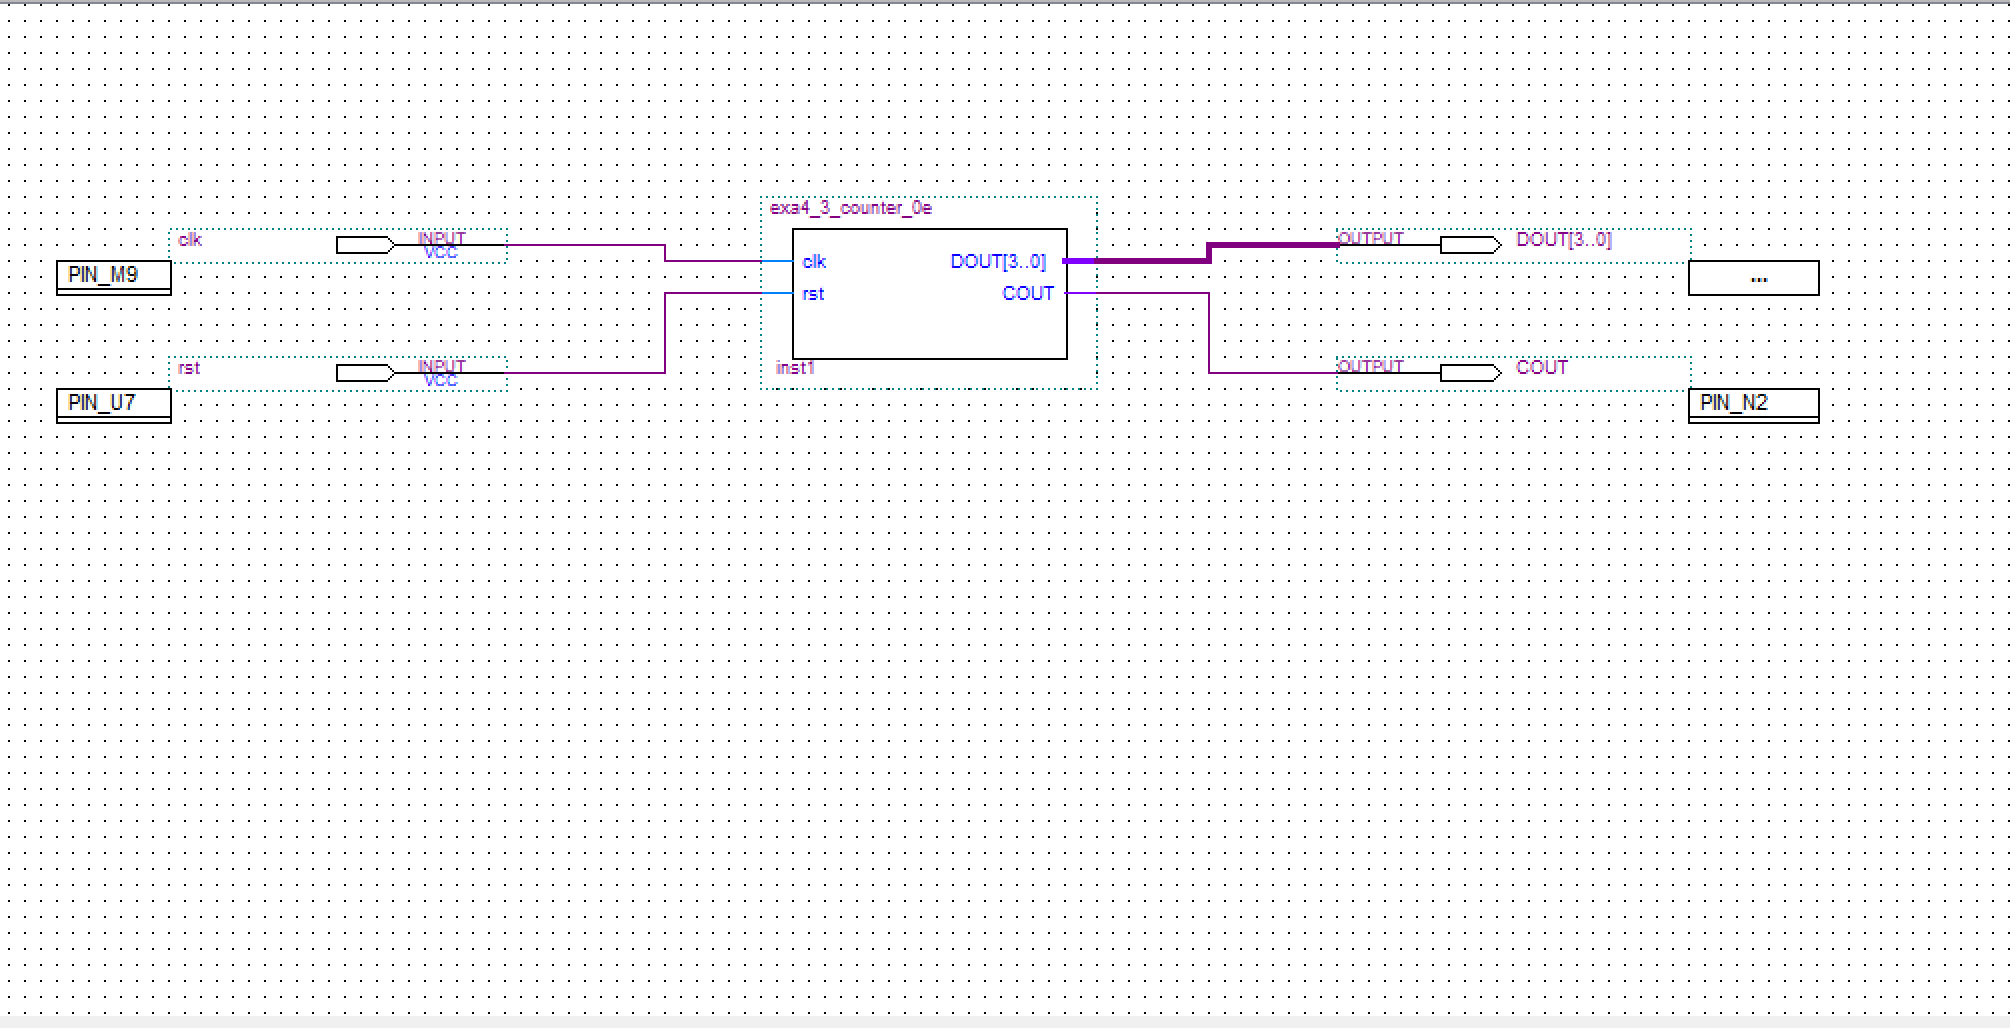
\includegraphics[width=0.75\textwidth]{要求3电路.png}
    \caption{要求 3 模 15 计数器 BDF 原理图}
    \label{e4:fig:task3_circuit}
\end{figure}

\subsubsection{波形仿真验证}

建立波形文件，设置时钟信号周期，在仿真开始时给复位端一个短暂的低电平脉冲。运行仿真后，观察 DOUT 依次输出 0, 1, 2, \ldots, 14, 0, 1, \ldots 的循环计数序列，COUT 在每次计数从 14 回到 0 时产生一个高电平脉冲，验证了计数器功能正确。

\subsection{要求 4：50M 分频器}

\subsubsection{创建工程与编写 VHDL}

新建工程，创建 VHDL 文件 \texttt{exa4\_4\_divider\_1hz\_10hz.vhd}，编写同时输出 1Hz 和 10Hz 的双路分频器。

\begin{minted}{vhdl}
library ieee;
use ieee.std_logic_1164.all;

entity exa4_4_divider_1hz_10hz is
generic(
    HALF_PERIOD_1HZ  : positive := 25000000;
    HALF_PERIOD_10HZ : positive := 2500000
);
port(
    clk50    : in  std_logic;
    clk_1hz  : out std_logic;
    clk_10hz : out std_logic
);
end exa4_4_divider_1hz_10hz;

architecture rtl of exa4_4_divider_1hz_10hz is
    signal cnt_1hz  : integer range 0 to HALF_PERIOD_1HZ - 1 := 0;
    signal cnt_10hz : integer range 0 to HALF_PERIOD_10HZ - 1 := 0;
    signal out_1hz  : std_logic := '0';
    signal out_10hz : std_logic := '0';
begin
    process(clk50)
    begin
        if rising_edge(clk50) then
            if cnt_1hz = HALF_PERIOD_1HZ - 1 then
                cnt_1hz <= 0;
                out_1hz <= not out_1hz;
            else
                cnt_1hz <= cnt_1hz + 1;
            end if;

            if cnt_10hz = HALF_PERIOD_10HZ - 1 then
                cnt_10hz <= 0;
                out_10hz <= not out_10hz;
            else
                cnt_10hz <= cnt_10hz + 1;
            end if;
        end if;
    end process;

    clk_1hz <= out_1hz;
    clk_10hz <= out_10hz;
end rtl;
\end{minted}
\captionof{listing}{双路分频器 VHDL 源码（exa4\_4\_divider\_1hz\_10hz.vhd）}
\label{e4:lst:divider}

分频器使用 \texttt{generic} 参数定义半周期计数值，使设计具有通用性。两路分频器共享同一个 \texttt{process}，各自独立计数。当计数达到半周期值时，输出信号翻转并重置计数，产生占空比 50\% 的方波。

\subsubsection{编译、生成原理图框图与建立顶层原理图}

编译后生成模块符号。在顶层 BDF 中放置分频器符号，连接输入时钟和两路输出。引脚分配如表~\ref{e4:tab:task4_pins} 所示，顶层原理图如图~\ref{e4:fig:task4_circuit} 所示。

\begin{table}[H]
    \centering
    \caption{要求 4 引脚分配表}
    \label{e4:tab:task4_pins}
    \begin{tabular}{ccc}
        \toprule
        \textbf{端口名} & \textbf{引脚} & \textbf{对应硬件} \\
        \midrule
        clk50     & PIN\_M9  & 50MHz 时钟 \\
        clk\_1hz  & PIN\_W2  & LEDR2 \\
        clk\_10hz & PIN\_AA1 & LEDR1 \\
        \bottomrule
    \end{tabular}
\end{table}

\begin{figure}[htbp]
    \centering
    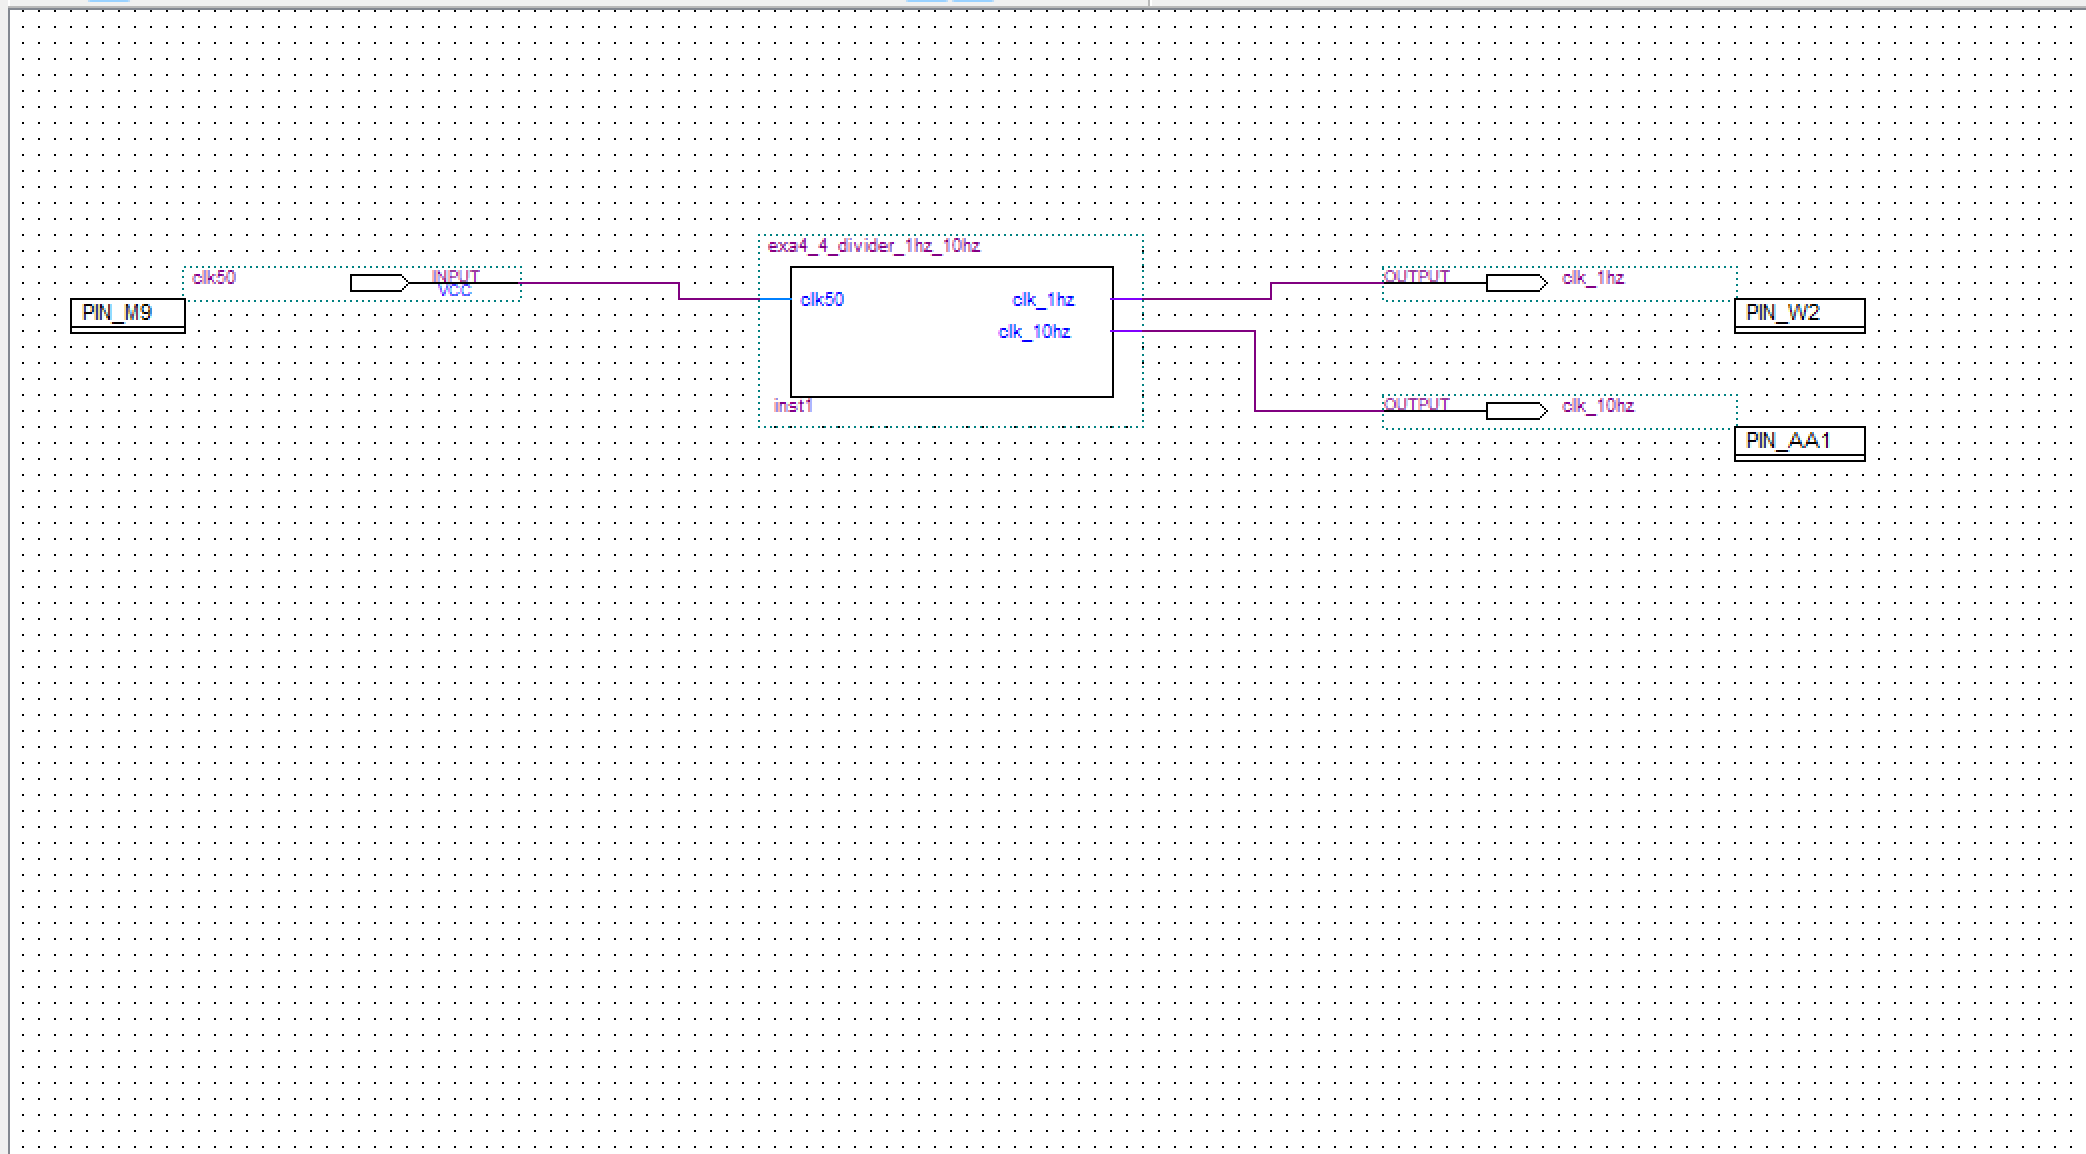
\includegraphics[width=0.75\textwidth]{要求4电路.png}
    \caption{要求 4 分频器 BDF 原理图}
    \label{e4:fig:task4_circuit}
\end{figure}

\subsubsection{仿真验证与下载验证}

由于使用实际分频参数（25,000,000 和 2,500,000）进行波形仿真需要极长的仿真时间，可通过编写测试台文件，使用 \texttt{generic map} 将半周期参数缩小（如设为 4 和 2），在较短的仿真时间内验证分频逻辑的正确性。

引脚分配完成后重新编译并下载到 DE0 开发板。利用板上 50MHz 晶振作为输入时钟，观察 LEDR2 以 1 秒为周期闪烁（1Hz），LEDR1 以 0.1 秒为周期闪烁（10Hz），验证分频器功能正确。

\subsection{要求 5：综合设计}

\subsubsection{设计方案}

综合设计需要在一个七段数码管上循环显示 12 位字符 \texttt{2539FEEL3980}，并在每轮显示结束后自动切换 1Hz 和 10Hz 的显示速度。整个系统由三个核心 VHDL 模块和一个顶层 BDF 原理图组成。

\subsubsection{编写 VHDL 模块}

\paragraph{特殊七段码译码器（exa4\_2\_2）}

该译码器根据要求 5 的显示序列进行定制，将计数值 0--11 映射到对应的七段显示码。

\begin{minted}{vhdl}
-- 七段码译码器：显示 2539FEEL3980
library ieee;
use ieee.std_logic_1164.all;

entity exa4_2_2 is
port(
    BCD_IN : in  std_logic_vector(3 downto 0);
    SG_OUT : out std_logic_vector(6 downto 0)
);
end exa4_2_2;

architecture one of exa4_2_2 is
begin
process(BCD_IN)
begin
    case BCD_IN is
        when "0000" => SG_OUT <= "0100100"; -- 2
        when "0001" => SG_OUT <= "0010010"; -- 5
        when "0010" => SG_OUT <= "0110000"; -- 3
        when "0011" => SG_OUT <= "0010000"; -- 9
        when "0100" => SG_OUT <= "0001110"; -- F
        when "0101" => SG_OUT <= "0000110"; -- E
        when "0110" => SG_OUT <= "0000110"; -- E
        when "0111" => SG_OUT <= "1000111"; -- L
        when "1000" => SG_OUT <= "0110000"; -- 3
        when "1001" => SG_OUT <= "0010000"; -- 9
        when "1010" => SG_OUT <= "0000000"; -- 8
        when "1011" => SG_OUT <= "1000000"; -- 0
        when others => SG_OUT <= "1111111";
    end case;
end process;
end one;
\end{minted}
\captionof{listing}{特殊七段码译码器（exa4\_2\_2.vhd）}
\label{e4:lst:decoder2}

\paragraph{M12 计数器（exa4\_3\_2）}

M12 计数器在模 15 计数器基础上修改为 0--11 循环，并新增使能信号 \texttt{en}，仅在使能有效时计数。

\begin{minted}{vhdl}
-- M12计数器：0~11循环，用于显示 2539FEEL3980 共12位
library ieee;
use ieee.std_logic_1164.all;
use ieee.numeric_std.all;

entity exa4_3_2 is
port(
    clk  : in  std_logic;
    rst  : in  std_logic;
    en   : in  std_logic;
    dout : out std_logic_vector(3 downto 0);
    cout : out std_logic
);
end exa4_3_2;

architecture one of exa4_3_2 is
signal Q1 : unsigned(3 downto 0) := (others => '0');
begin

process(clk, rst)
begin
    if rst = '0' then
        Q1 <= (others => '0');
        cout <= '0';

    elsif rising_edge(clk) then
        cout <= '0';

        if en = '1' then
            if Q1 = to_unsigned(11, 4) then
                Q1 <= (others => '0');
                cout <= '1';
            else
                Q1 <= Q1 + 1;
            end if;
        end if;
    end if;
end process;

dout <= std_logic_vector(Q1);

end one;
\end{minted}
\captionof{listing}{M12 计数器（exa4\_3\_2.vhd）}
\label{e4:lst:counter2}

\paragraph{自动 1Hz/10Hz 切换控制器（exa4\_auto\_1hz\_10hz）}

该模块集成了分频和速度切换功能。内部维护一个模式标志 \texttt{mode}（0 表示 1Hz，1 表示 10Hz），每当收到 M12 计数器的 \texttt{loop\_end} 信号时切换模式。根据当前模式选择不同的分频系数，产生对应频率的 \texttt{tick} 脉冲。

\begin{minted}{vhdl}
-- 1Hz / 10Hz 自动切换tick发生器
library ieee;
use ieee.std_logic_1164.all;

entity exa4_auto_1hz_10hz is
port(
    clk50     : in  std_logic;
    rst       : in  std_logic;
    loop_end  : in  std_logic;
    tick      : out std_logic;
    speed_sel : out std_logic
);
end exa4_auto_1hz_10hz;

architecture rtl of exa4_auto_1hz_10hz is

constant DIV_1HZ  : integer := 50000000;
constant DIV_10HZ : integer := 5000000;

signal cnt    : integer range 0 to DIV_1HZ - 1 := 0;
signal mode   : std_logic := '0';
signal tick_r : std_logic := '0';

begin

process(clk50, rst)
    variable limit_v : integer;
begin
    if rst = '0' then
        cnt    <= 0;
        mode   <= '0';
        tick_r <= '0';

    elsif rising_edge(clk50) then
        tick_r <= '0';

        if loop_end = '1' then
            mode <= not mode;
            cnt  <= 0;

        else
            if mode = '0' then
                limit_v := DIV_1HZ - 1;
            else
                limit_v := DIV_10HZ - 1;
            end if;

            if cnt >= limit_v then
                cnt    <= 0;
                tick_r <= '1';
            else
                cnt <= cnt + 1;
            end if;
        end if;
    end if;
end process;

tick <= tick_r;
speed_sel <= mode;

end rtl;
\end{minted}
\captionof{listing}{自动 1Hz/10Hz 切换控制器（exa4\_auto\_1hz\_10hz.vhd）}
\label{e4:lst:auto}

\subsubsection{生成原理图框图}

对上述三个 VHDL 模块分别进行编译，然后通过 \textbf{File $\rightarrow$ Create/Update $\rightarrow$ Create Symbol Files for Current File} 生成各自的 \texttt{.bsf} 模块符号文件，使其可在顶层原理图中作为元件调用。

\subsubsection{建立顶层原理图与引脚分配}

新建 BDF 原理图文件作为顶层设计，从 Project 元件库中依次放置三个模块符号，按照以下连接关系完成布线：

\begin{itemize}
    \item 50MHz 时钟（PIN\_M9）同时连接到 \texttt{exa4\_auto\_1hz\_10hz} 的 \texttt{clk50} 端和 \texttt{exa4\_3\_2} 的 \texttt{clk} 端。
    \item 复位信号（PIN\_U13，按键 SW0）同时连接到两个模块的 \texttt{rst} 端。
    \item \texttt{exa4\_auto\_1hz\_10hz} 的 \texttt{tick} 输出连接到 \texttt{exa4\_3\_2} 的 \texttt{en} 输入。
    \item \texttt{exa4\_3\_2} 的 \texttt{dout[3:0]} 连接到 \texttt{exa4\_2\_2} 的 \texttt{BCD\_IN[3:0]}。
    \item \texttt{exa4\_3\_2} 的 \texttt{cout} 反馈连接到 \texttt{exa4\_auto\_1hz\_10hz} 的 \texttt{loop\_end} 输入。
    \item \texttt{exa4\_2\_2} 的 \texttt{SG\_OUT[6:0]} 连接到 HEX0 数码管输出引脚。
\end{itemize}

引脚分配如表~\ref{e4:tab:task5_pins} 所示，顶层原理图如图~\ref{e4:fig:task5_circuit} 所示。

\begin{table}[H]
    \centering
    \caption{要求 5 引脚分配表}
    \label{e4:tab:task5_pins}
    \begin{tabular}{ccc}
        \toprule
        \textbf{端口名} & \textbf{引脚} & \textbf{对应硬件} \\
        \midrule
        clk50 (pin\_name4) & PIN\_M9  & 50MHz 时钟 \\
        rst (pin\_name5)   & PIN\_U13 & SW0 \\
        SG\_OUT[6]         & PIN\_AA22 & HEX0[6] \\
        SG\_OUT[5]         & PIN\_Y21  & HEX0[5] \\
        SG\_OUT[4]         & PIN\_Y22  & HEX0[4] \\
        SG\_OUT[3]         & PIN\_W21  & HEX0[3] \\
        SG\_OUT[2]         & PIN\_W22  & HEX0[2] \\
        SG\_OUT[1]         & PIN\_V21  & HEX0[1] \\
        SG\_OUT[0]         & PIN\_U21  & HEX0[0] \\
        \bottomrule
    \end{tabular}
\end{table}

\begin{figure}[htbp]
    \centering
    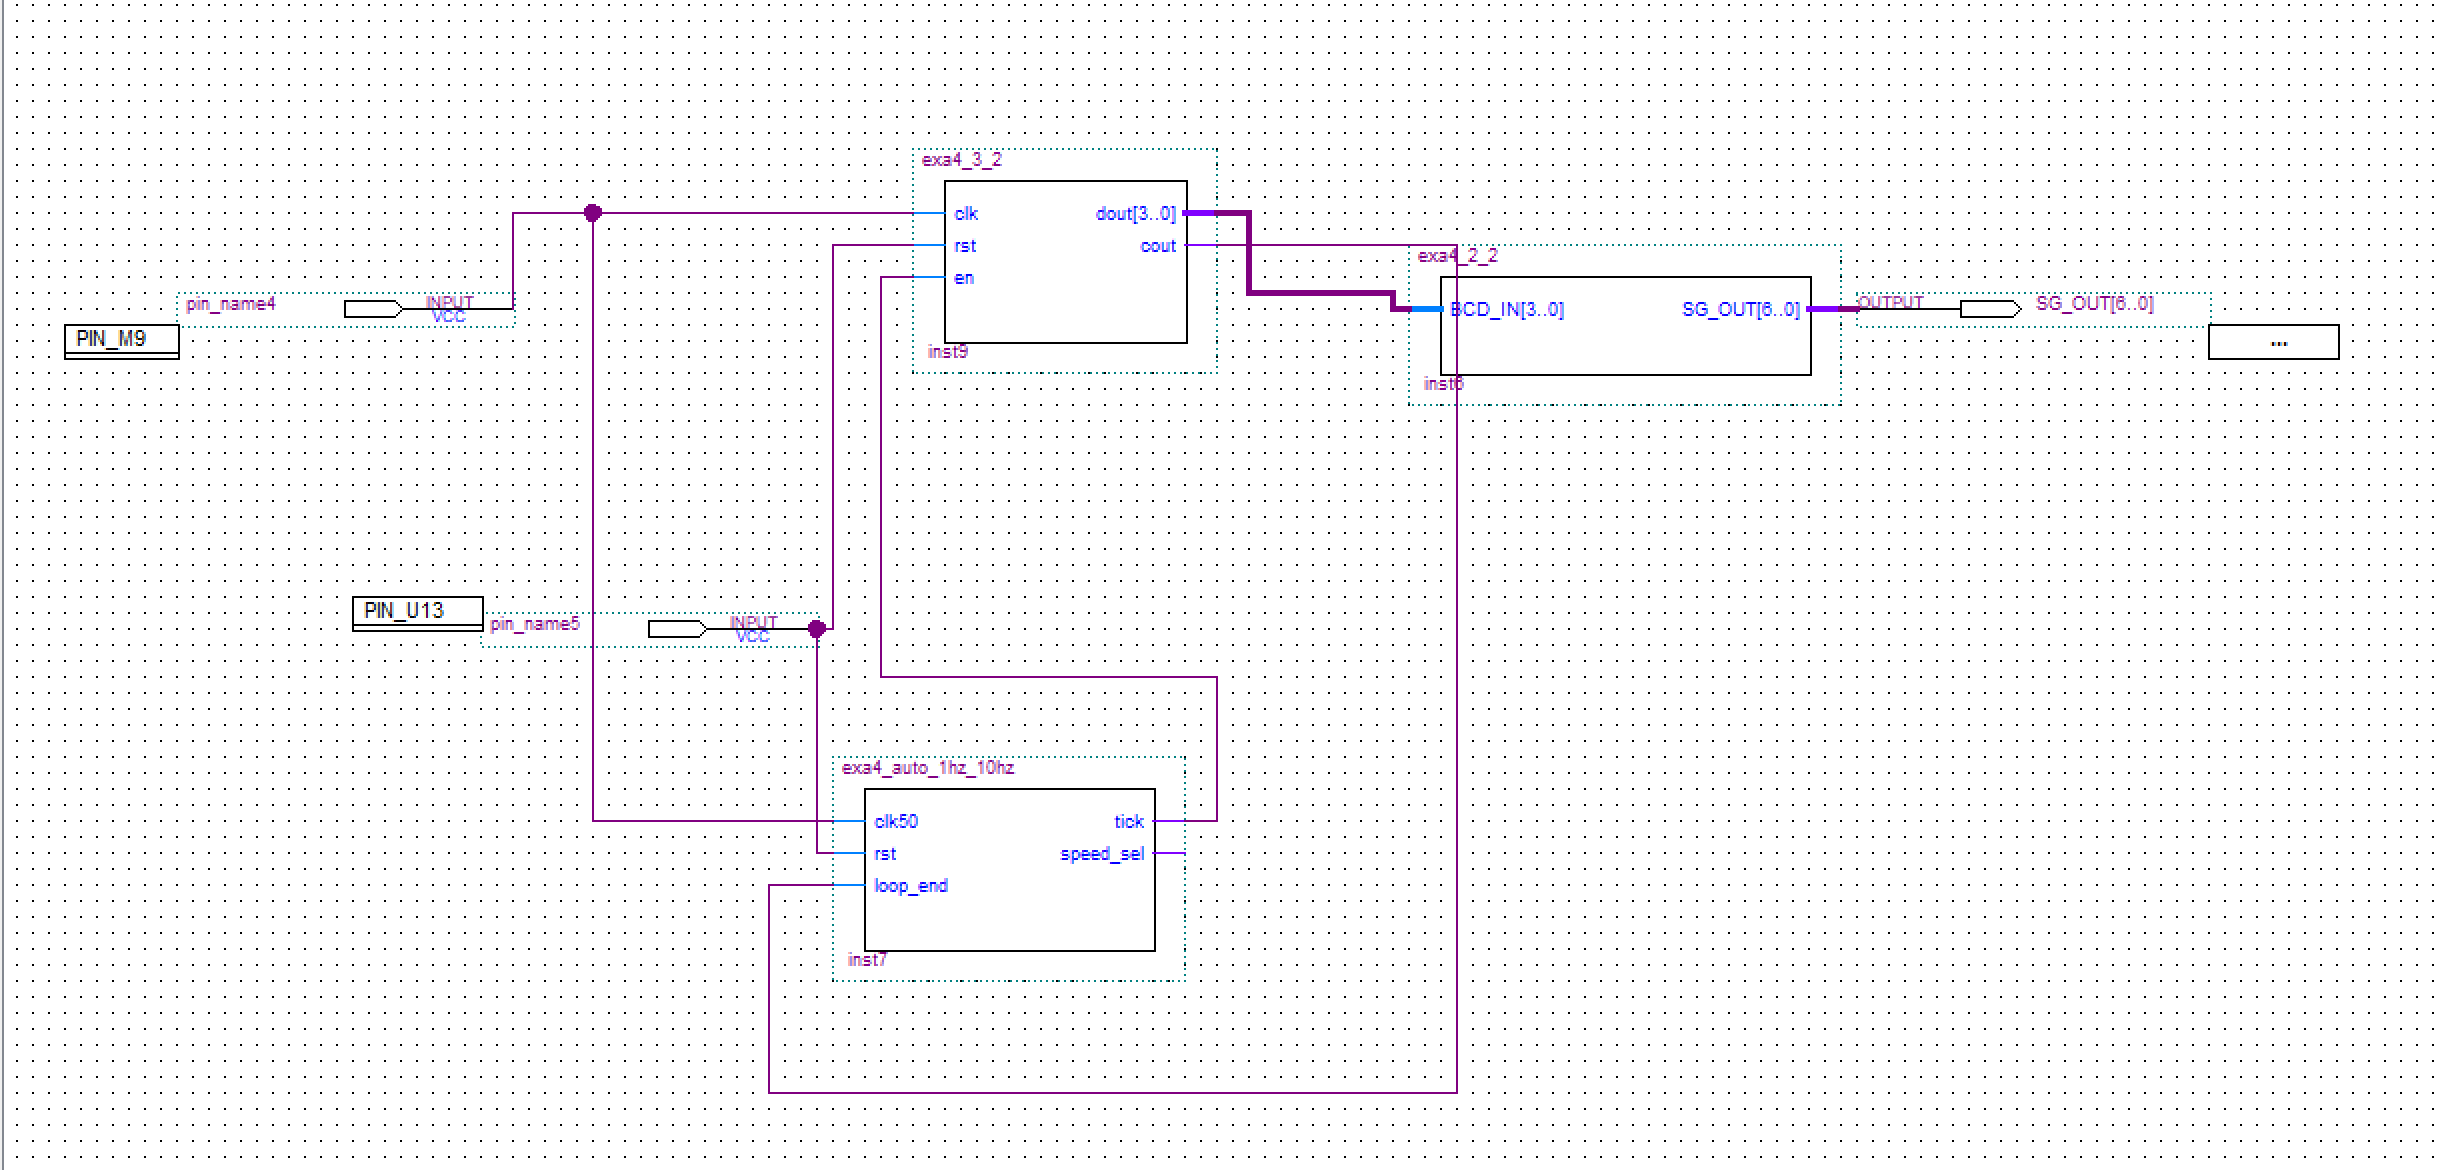
\includegraphics[width=0.75\textwidth]{要求5电路.png}
    \caption{要求 5 综合设计 BDF 原理图}
    \label{e4:fig:task5_circuit}
\end{figure}

\subsubsection{编译与下载验证}

将 BDF 原理图文件设置为顶层实体，进行完整编译。确认编译无错误后，通过 USB-Blaster 以 JTAG 模式下载到 DE0 开发板。

下载完成后，观察 HEX0 数码管的显示行为：数码管以 1Hz 的速度依次显示 2, 5, 3, 9, F, E, E, L, 3, 9, 8, 0 共 12 个字符，完成一轮后自动切换到 10Hz 速度进行下一轮循环显示，然后再切回 1Hz，如此交替进行。按下复位键可使显示从第一个字符重新开始。

\section{实验过程中的问题}

\begin{enumerate}
    \item \textbf{VHDL 模块生成原理图框图}：本实验首次使用 VHDL 描述电路模块。初次操作时不清楚如何将 VHDL 文件变为可在 BDF 原理图中调用的元件。关键步骤是编译 VHDL 文件后，选择 File $\rightarrow$ Create/Update $\rightarrow$ Create Symbol Files for Current File 生成 \texttt{.bsf} 符号文件。若跳过此步骤，在元件库中将找不到对应模块。
    \item \textbf{分频器仿真时间过长}：使用实际半周期参数（25,000,000）进行波形仿真时，即使只观察一个完整周期也需要模拟 5000 万个时钟周期，仿真耗时极长。解决方法是编写测试台文件，通过 \texttt{generic map} 将半周期参数缩小为较小的值（如 4 和 2），在合理的仿真时间内验证分频逻辑是否正确。
    \item \textbf{七段数码管有效电平}：DE0 开发板的七段数码管为共阳极结构，段选信号低电平有效（输出 0 点亮对应段，输出 1 熄灭对应段）。若译码器的段选编码极性错误，数码管上所有笔段会出现反转显示。本实验的 VHDL 代码中已按低电平有效编码，可直接驱动数码管。
    \item \textbf{综合设计中模块间的反馈连接}：要求 5 中，M12 计数器的 \texttt{cout} 输出需反馈到自动切换控制器的 \texttt{loop\_end} 输入，而控制器的 \texttt{tick} 输出又连接到计数器的 \texttt{en} 输入，形成闭环。若任一反馈连线缺失，系统将无法正常工作：缺少 \texttt{tick} 连接时计数器不会计数，缺少 \texttt{cout} 反馈时速度无法切换。
\end{enumerate}

\section{心得体会}

\begin{enumerate}
    \item 通过本次实验，我初步掌握了 VHDL 硬件描述语言的基本语法和设计方法。与前几次实验中使用的原理图输入方式相比，VHDL 能够用简洁的文字代码描述复杂的逻辑功能，尤其在实现译码器、计数器等功能模块时，代码方式比手工连线更加高效且不易出错。
    \item 本实验从简单的异或门出发，逐步过渡到译码器、计数器、分频器，最终完成多模块综合设计，让我深刻体会到模块化设计的思想。每个功能模块可以独立设计、独立仿真验证，确认正确后再在顶层进行集成，大大降低了复杂系统的调试难度。
    \item 要求 5 的综合设计将 VHDL 文本描述与 BDF 图形化连接相结合，发挥了两种设计方法各自的优势：VHDL 适合描述功能逻辑，BDF 原理图适合展示模块间的连接关系和信号流向。这种混合设计方法在实际的 FPGA 工程开发中也是常用的实践方式。
\end{enumerate}

% ==================== 实验5：基于 ROM 的波形发生与字符显示系统 ====================
\graphicspath{{../5. rom/figures/}}
\chapter{基于 ROM 的波形发生与字符显示系统}

\section{实验目的}

\begin{enumerate}
    \item 掌握只读存储器 ROM 在数字系统中的应用，熟悉 Quartus II 中 ROM IP 核 \texttt{altsyncram} 的配置流程和 \texttt{.mif} 文件的数据初始化方法。
    \item 理解用计数器扫描 ROM 地址来顺序输出数据的设计思路，掌握用 ROM 查表产生正弦波、显示字符序列的原理。
    \item 学会把分频器、计数器、ROM、译码器组合成一个系统，先用 VHDL 编写各功能模块，再用原理图把它们连接起来，完成混合设计。
    \item 学会用拨码开关和门电路实现模式切换，并在 DE0 开发板上用 LED 和七段数码管验证结果。
\end{enumerate}

\section{实验要求}

本次实验的要求以现场给出的实验内容为准，具体如下：

\begin{enumerate}
    \item \textbf{要求 1}：配置一块宽度为 8 位的 ROM，在其中存储 512 个地址的正弦波数据。以系统时钟作为计数器的计数脉冲，用 74161 一类的计数器模块、或用硬件描述语言编写的计数模块，让其输出依次扫描 ROM 的地址端，把 ROM 中保存的数据按 1\,Hz 的频率输出，通过 DE0 开发板上的 8 位 LED 灯查看并验证。
    \item \textbf{要求 2}：配置一块存储学号的 ROM，学号内容取同学 A 的后 4 位学号，接上 F、L、E、P，再接同学 B 的后 3 位学号。用计数器的输出依次扫描 ROM 的地址端，把数据按 1\,Hz 的频率输出，通过 DE0 开发板上的 1 个七段数码管查看并验证。
    \item \textbf{要求 3}：要求 2 与要求 1 通过控制开关切换。
\end{enumerate}

本组两名同学中，同学 A 庞铭洋的学号为 2024302539，同学 B 郭浩然的学号为 2024303980。按要求 2 的规则，同学 A 的后 4 位是 \texttt{2539}，同学 B 的后 3 位是 \texttt{980}，中间插入 F、L、E、P，因此本组要在七段数码管上循环显示的字符序列为 \texttt{2539FLEP980}，一共 11 个字符。

\section{实验设备}

\begin{itemize}
    \item Quartus II 开发软件，含 MegaWizard Plug-In Manager 和 ROM IP 核
    \item DE0 开发板，FPGA 型号为 Cyclone V 5CEBA4F23C7
    \item USB-Blaster 下载线及计算机
    \item 板载 50\,MHz 晶振、拨码开关、8 个红色 LED 灯 LEDR 和七段数码管 HEX0
\end{itemize}

\section{实验原理}

\subsection{ROM 存储器原理}

只读存储器 ROM 是一种非易失性存储器，写入之后内容只能读出，不能在运行过程中修改。它的工作方式就是查表：把地址作为索引送进去，ROM 就把该地址上事先存好的数据读出来，即
\[
    \mathrm{data\_out} = \mathrm{ROM}[\mathrm{addr}].
\]

本实验的 ROM 用 Quartus II 自带的 \texttt{altsyncram} IP 核实现，在 MegaWizard Plug-In Manager 里可以直接设定数据宽度、存储深度和初始化文件 \texttt{.mif}，综合后由 FPGA 内部的 M10K 嵌入式存储块承担。本实验用到两块 ROM：

\begin{itemize}
    \item \textbf{正弦波 ROM} \texttt{sinrom}：数据宽度 8 位，深度 512 字，地址位宽取 9 位，对应 $2^9 = 512$ 个地址；初始化文件是 \texttt{dds\_512x8b\_wave.mif}，存的是一个完整周期正弦波的 512 点等间隔采样，数值在 $0\sim255$ 之间，零点偏置约为 128。
    \item \textbf{学号字符 ROM} \texttt{xuehaoHOPE}：数据宽度 4 位，深度 32 字，地址位宽 5 位；初始化文件是 \texttt{Mif1.mif}，地址 $0\sim10$ 这 11 个单元存放待显示字符的 4 位编码索引，其余地址填 0。
\end{itemize}

\subsection{计数器扫描与查表式波形发生原理}

ROM 只负责把地址映射成数据。要让数据按时间顺序自动输出，还需要一个地址计数器不断地把 ROM 的地址从头扫到尾。计数器在扫描时钟驱动下从 0 加到最大地址再归零，ROM 输出端就按存储顺序循环送出各个采样点，存进去的波形或字符序列也就在输出端重建出来。直接数字频率合成 DDS 产生任意波形，依靠的正是这种存采样、扫地址的方法。

\begin{itemize}
    \item 正弦波模式用一个模 512 计数器产生 $0\sim511$ 的 9 位地址，逐点扫过正弦波 ROM，把 512 个采样值依次送到 8 位 LED 上，LED 的亮灭组合就反映出正弦幅值的周期变化。
    \item 学号模式用一个模 11 计数器产生 $0\sim10$ 的地址，循环扫描学号 ROM 的 11 个有效单元，输出经七段译码后在数码管上循环显示这 11 个字符。
\end{itemize}

\subsection{分频原理}

DE0 开发板的系统时钟是 50\,MHz，若直接用它作扫描时钟，LED 和数码管刷新太快，肉眼无法分辨，所以要先分频，把扫描频率降到 1\,Hz 上下。分频就是对高频时钟计数：设输入频率为 $f_{\text{clk}}$、期望输出频率为 $f_{\text{out}}$，要得到占空比 50\% 的方波，半周期需要的计数值为
\[
    N = \frac{f_{\text{clk}}}{2 \times f_{\text{out}}}.
\]
把 50\,MHz 分到 1\,Hz 时，$N = 50{,}000{,}000 / 2 = 25{,}000{,}000$。顶层把这一步交给 \texttt{lpm\_counter0} 完成，它是一个 26 位的 LPM 计数器 IP，对系统时钟分频后取出一路低速脉冲，作为约 1\,Hz 量级的扫描时钟去驱动后面的电路。

\subsection{模式切换原理}

两种模式共用同一路分频后的扫描时钟，由拨码开关 \texttt{switch} 决定让哪条数据通路工作。顶层用一个反相器和两个二输入与门，把扫描时钟分别门控到两条通路上，逻辑见表~\ref{e5:tab:mode}。哪条通路被关闭，它的计数器就停止计数，对应 ROM 的寄存输出保持原值，两条通路互不影响。两个计数器的复位端 \texttt{RST} 都接高电平 VCC，也就是始终不复位、保持正常计数。

\begin{table}[H]
    \centering
    \caption{模式切换功能对照表}
    \label{e5:tab:mode}
    \begin{tabular}{cccc}
        \toprule
        \textbf{switch} & \textbf{工作模式} & \textbf{扫描时钟使能的通路} & \textbf{现象} \\
        \midrule
        0 & 正弦波模式   & \texttt{Vhd1}+\texttt{sinrom}     & 8 位 LED 显示正弦采样；数码管保持不变 \\
        1 & 学号序列模式 & \texttt{time2}+\texttt{xuehaoHOPE} & 数码管循环显示学号字符；LED 保持 0 \\
        \bottomrule
    \end{tabular}
\end{table}

\subsection{七段数码管译码原理}

学号 ROM 送出的是 4 位编码索引，要先经七段译码器 \texttt{bin2seg} 转换成 7 位段选信号才能驱动数码管。DE0 板上的七段数码管是共阳极结构，段选信号低电平有效，即某段给 0 点亮、给 1 熄灭。编码索引与显示字符的对应关系见表~\ref{e5:tab:bin2seg}。

\begin{table}[H]
    \centering
    \caption{\texttt{bin2seg} 七段译码真值表，段序 abcdefg、低电平有效}
    \label{e5:tab:bin2seg}
    \begin{tabular}{ccc}
        \toprule
        \textbf{bin\_input[3:0]} & \textbf{seg\_output[6:0]} & \textbf{显示字符} \\
        \midrule
        0000 & 0010010 & 5 \\
        0001 & 0110000 & 3 \\
        0010 & 0010000 & 9 \\
        0011 & 0001110 & F \\
        0100 & 1000111 & L \\
        0101 & 0000110 & E \\
        0110 & 0001100 & P \\
        0111 & 0010000 & 9 \\
        1000 & 0000000 & 8 \\
        1001 & 1000000 & 0 \\
        1010 & 0100100 & 2 \\
        其他 & 1111111 & 全灭 \\
        \bottomrule
    \end{tabular}
\end{table}

\section{实验内容}

本系统把 VHDL 文本设计和原理图设计结合起来：各功能子模块用 VHDL 编写，编译后生成原理图符号，再在顶层原理图中调用、连线，拼成完整系统。整个软件流程是：建立工程，用 MegaWizard 配置两块 ROM IP 核，编写各子模块 VHDL 代码并生成符号，绘制顶层原理图，编译，波形仿真，引脚分配，最后下载到开发板验证。

\subsection{建立工程与配置 ROM IP 核}

打开 Quartus II，用 \textbf{File $\rightarrow$ New Project Wizard} 新建工程，器件选 DE0 开发板对应的 Cyclone V \texttt{5CEBA4F23C7}。随后打开 \textbf{Tools $\rightarrow$ MegaWizard Plug-In Manager}，按 \texttt{ROM: 1-PORT} 类型配置两块 ROM IP 核：

\begin{enumerate}
    \item \textbf{正弦波 ROM \texttt{sinrom}}：输出位宽设为 8 位，深度设为 512 字，地址 9 位，勾选用 \texttt{.mif} 文件初始化并指定 \texttt{dds\_512x8b\_wave.mif}。这个 \texttt{.mif} 里的 512 点正弦采样不是手工填的，而是用波形转换工具 \texttt{WaveToMif} 从一个周期的正弦波生成，幅值范围 $0\sim255$。前几个采样值列在表~\ref{e5:tab:sinmif}。
    \item \textbf{学号字符 ROM \texttt{xuehaoHOPE}}：输出位宽设为 4 位，深度设为 32 字，用 \texttt{Mif1.mif} 初始化。\texttt{Mif1.mif} 的内容以及经 \texttt{bin2seg} 译码后显示的字符见表~\ref{e5:tab:xuehaomif}。
\end{enumerate}

\begin{table}[H]
    \centering
    \caption{正弦波 ROM 初始化文件 \texttt{dds\_512x8b\_wave.mif} 部分采样值}
    \label{e5:tab:sinmif}
    \begin{tabular}{cccccccccc}
        \toprule
        地址 & 0 & 1 & 2 & 3 & 4 & 5 & 6 & 7 & $\cdots$ \\
        \midrule
        十进制数据 & 127 & 128 & 130 & 131 & 133 & 134 & 136 & 137 & $\cdots$ \\
        \bottomrule
    \end{tabular}
\end{table}

\begin{table}[H]
    \centering
    \caption{学号字符 ROM 初始化文件 \texttt{Mif1.mif} 内容与显示映射}
    \label{e5:tab:xuehaomif}
    \begin{tabular}{cccc}
        \toprule
        \textbf{ROM 地址} & \textbf{存储的 4 位编码} & \textbf{经 \texttt{bin2seg} 译码} & \textbf{显示字符} \\
        \midrule
        0  & 1010 & 0100100 & 2 \\
        1  & 0000 & 0010010 & 5 \\
        2  & 0001 & 0110000 & 3 \\
        3  & 0010 & 0010000 & 9 \\
        4  & 0011 & 0001110 & F \\
        5  & 0100 & 1000111 & L \\
        6  & 0101 & 0000110 & E \\
        7  & 0110 & 0001100 & P \\
        8  & 0111 & 0010000 & 9 \\
        9  & 1000 & 0000000 & 8 \\
        10 & 1001 & 1000000 & 0 \\
        11--31 & 0000 & --- & 未使用 \\
        \bottomrule
    \end{tabular}
\end{table}

把地址 $0\sim10$ 顺序读出后，数码管上正好显示 \texttt{2539FLEP980}，与要求 2 一致。

\subsection{编写各子模块 VHDL 代码}

\subsubsection{模 512 地址计数器 Vhd1}

\texttt{Vhd1} 负责产生正弦波 ROM 的 9 位地址。扫描时钟每来一个上升沿就计数加 1，数到 511 后归零，同时给出一个进位脉冲 \texttt{COUT}，这样循环扫完 512 个地址；\texttt{RST} 为低电平时异步清零。

\begin{minted}{vhdl}
LIBRARY IEEE;
USE IEEE.STD_LOGIC_1164.ALL;
USE IEEE.STD_LOGIC_UNSIGNED.ALL;
ENTITY Vhd1 IS
    PORT ( clk,RST : IN  STD_LOGIC;
           DOUT    : OUT STD_LOGIC_VECTOR (8 DOWNTO 0);  -- 9位计数
           COUT    : OUT STD_LOGIC);                      -- 进位位
END Vhd1;
ARCHITECTURE fwm OF Vhd1 IS
    SIGNAL Q1 : STD_LOGIC_VECTOR (8 DOWNTO 0);
BEGIN
PROCESS(clk,RST)
BEGIN
    IF RST = '0' THEN
        Q1 <= (OTHERS => '0'); COUT <= '0';
    ELSIF clk'EVENT AND clk = '1' THEN
        Q1 <= Q1 + 1;
        COUT <= '0';
        IF Q1 >= "111111111" THEN          -- 计满 511 归零
            Q1 <= (OTHERS => '0'); COUT <= '1';
        END IF;
    END IF;
END PROCESS;
DOUT <= Q1;
END fwm;
\end{minted}
\captionof{listing}{模 512 地址计数器 Vhd1.vhd}
\label{e5:lst:vhd1}

\subsubsection{模 11 地址计数器 time2}

\texttt{time2} 负责产生学号 ROM 的地址，计数范围 $0\sim10$，对应 11 个有效字符，数到 10 后下一拍归零，做成 11 进制循环计数。

\begin{minted}{vhdl}
LIBRARY IEEE;
USE IEEE.STD_LOGIC_1164.ALL;
USE IEEE.STD_LOGIC_UNSIGNED.ALL;
ENTITY time2 IS
    PORT ( clk,RST : IN  STD_LOGIC;
           DOUT    : OUT STD_LOGIC_VECTOR (4 DOWNTO 0);  -- 五位计数
           COUT    : OUT STD_LOGIC);                      -- 进位位
END time2;
ARCHITECTURE fwm OF time2 IS
    SIGNAL Q1 : STD_LOGIC_VECTOR (4 DOWNTO 0);
BEGIN
    PROCESS(clk,RST)
    BEGIN
        IF RST = '0' THEN
            Q1 <= (OTHERS => '0'); COUT <= '0';
        ELSIF clk'EVENT AND clk = '1' THEN
            Q1 <= Q1 + 1;
            COUT <= '0';
            IF Q1 >= "01010" THEN          -- 计到 10 归零
                Q1 <= (OTHERS => '0'); COUT <= '1';
            END IF;
        END IF;
    END PROCESS;
    DOUT <= Q1;
END fwm;
\end{minted}
\captionof{listing}{模 11 地址计数器 time2.vhd}
\label{e5:lst:time2}

\subsubsection{七段数码管译码器 bin2seg}

\texttt{bin2seg} 接收学号 ROM 输出的 4 位编码，用 \texttt{case} 语句映射成共阳极七段码，低电平有效，实现表~\ref{e5:tab:bin2seg} 中的字符显示。

\begin{minted}{vhdl}
library IEEE;
use IEEE.STD_LOGIC_1164.ALL;
entity bin2seg is
    Port ( bin_input  : in  STD_LOGIC_VECTOR(3 downto 0);  -- 4位二进制输入
           seg_output : out STD_LOGIC_VECTOR(6 downto 0)); -- 七段输出(abcdefg)
end bin2seg;
architecture Behavioral of bin2seg is
begin
    process(bin_input)
    begin
        case bin_input is                  -- 共阳极数码管段码（低电平有效）
            when "0000" => seg_output <= "0010010"; -- 5
            when "0001" => seg_output <= "0110000"; -- 3
            when "0010" => seg_output <= "0010000"; -- 9
            when "0011" => seg_output <= "0001110"; -- F
            when "0100" => seg_output <= "1000111"; -- L
            when "0101" => seg_output <= "0000110"; -- E
            when "0110" => seg_output <= "0001100"; -- P
            when "0111" => seg_output <= "0010000"; -- 9
            when "1000" => seg_output <= "0000000"; -- 8
            when "1001" => seg_output <= "1000000"; -- 0
            when "1010" => seg_output <= "0100100"; -- 2
            when others => seg_output <= "1111111"; -- 全灭
        end case;
    end process;
end Behavioral;
\end{minted}
\captionof{listing}{七段数码管译码器 bin2seg.vhd}
\label{e5:lst:bin2seg}

分频功能由 \texttt{lpm\_counter0} 这个 26 位 LPM 计数器 IP 完成。把上面几个 VHDL 模块分别编译，再用 \textbf{File $\rightarrow$ Create/Update $\rightarrow$ Create Symbol Files for Current File} 各自生成 \texttt{.bsf} 符号，连同两块 ROM IP 的符号一起供顶层原理图调用。

\subsection{绘制顶层原理图}

新建一个 BDF 原理图作为顶层设计，把各模块符号放上去，按下面的关系连线，顶层原理图如图~\ref{e5:fig:top}。

\begin{itemize}
    \item 输入有两个：\texttt{clk} 接板载 50\,MHz 系统时钟，\texttt{switch} 接模式选择拨码开关。
    \item \texttt{lpm\_counter0} 以 \texttt{clk} 为时钟，对系统时钟分频，得到低速扫描时钟。
    \item \texttt{switch} 经反相器取反后与扫描时钟相与，得到正弦波通路的时钟，驱动 \texttt{Vhd1} 和 \texttt{sinrom}；\texttt{switch} 不取反、直接与扫描时钟相与，得到学号通路的时钟，驱动 \texttt{time2} 和 \texttt{xuehaoHOPE}。两个计数器的 \texttt{RST} 都接 VCC，始终不复位。
    \item \texttt{Vhd1} 的 \texttt{DOUT[8..0]} 接 \texttt{sinrom} 的 \texttt{address[8..0]}，\texttt{sinrom} 的 \texttt{q[7..0]} 接 8 位输出 \texttt{led[7..0]}。
    \item \texttt{time2} 的 \texttt{DOUT[4..0]} 接 \texttt{xuehaoHOPE} 的 \texttt{address[4..0]}，\texttt{xuehaoHOPE} 的 \texttt{q[3..0]} 接 \texttt{bin2seg} 的 \texttt{bin\_input[3..0]}，译码输出 \texttt{seg\_output[6..0]} 拆分为 7 个段选输出 \texttt{A,b,c,d,e,f,g} 接七段数码管 HEX0。
\end{itemize}

\begin{figure}[htbp]
    \centering
    
\includegraphics[width=0.75\textwidth]{电路图.png}
    \caption{基于 ROM 的波形发生与字符显示系统顶层原理图}
    \label{e5:fig:top}
\end{figure}

\subsection{编译与波形仿真}

把 BDF 文件设成顶层实体，完整编译一遍。实际分频系数很大，若照真实时钟仿真要花很长时间，所以仿真时先把扫描时钟的分频比临时调小，让计数器快速扫完 ROM，在可接受的时间内把逻辑验证清楚；下载到开发板时再把分频比改回去，恢复约 1\,Hz 的实际扫描频率。

\subsubsection{正弦波模式仿真}

把 \texttt{switch} 置 0，新建波形文件，加入 \texttt{clk}、\texttt{switch}、\texttt{led[7..0]} 等信号运行功能仿真，结果如图~\ref{e5:fig:sim1}。

\begin{figure}[htbp]
    \centering
    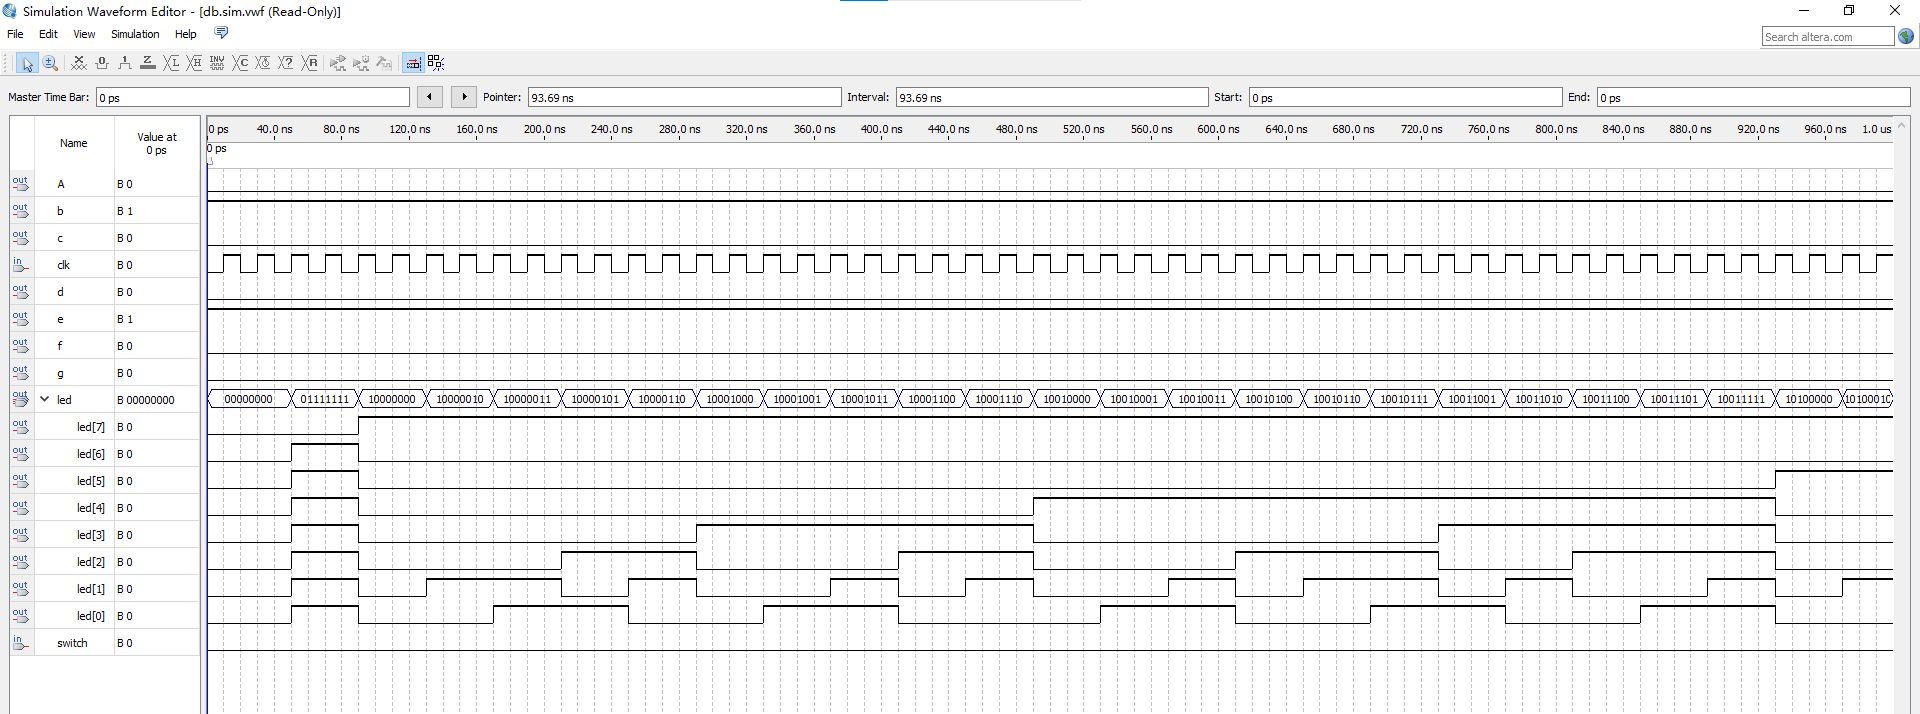
\includegraphics[width=0.75\textwidth]{任务1仿真.png}
    \caption{switch = 0 时的正弦波模式功能仿真波形}
    \label{e5:fig:sim1}
\end{figure}

\texttt{switch} 一直保持低电平，系统处于正弦波输出模式。\texttt{led[7..0]} 从初值 \texttt{00000000} 起，随 \texttt{Vhd1} 的地址递增依次输出 \texttt{01111111}、\texttt{10000000}、\texttt{10000010}、\texttt{10000011}、\texttt{10000101}、\texttt{10000110} 等，换算成十进制就是 127、128、130、131、133、134，数值一路上升，与表~\ref{e5:tab:sinmif} 中 \texttt{dds\_512x8b\_wave.mif} 预存的采样值逐一吻合，说明正弦波 ROM 的地址扫描和数据输出都正确。这时学号通路的时钟被关闭，数码管段选保持在地址 0 对应的字符 \texttt{2} 上不变。

\subsubsection{学号序列模式仿真}

把 \texttt{switch} 置 1，加入七段输出 \texttt{A,b,c,d,e,f,g} 和 \texttt{led} 等信号再运行一次仿真，结果如图~\ref{e5:fig:sim2}。

\begin{figure}[htbp]
    \centering
    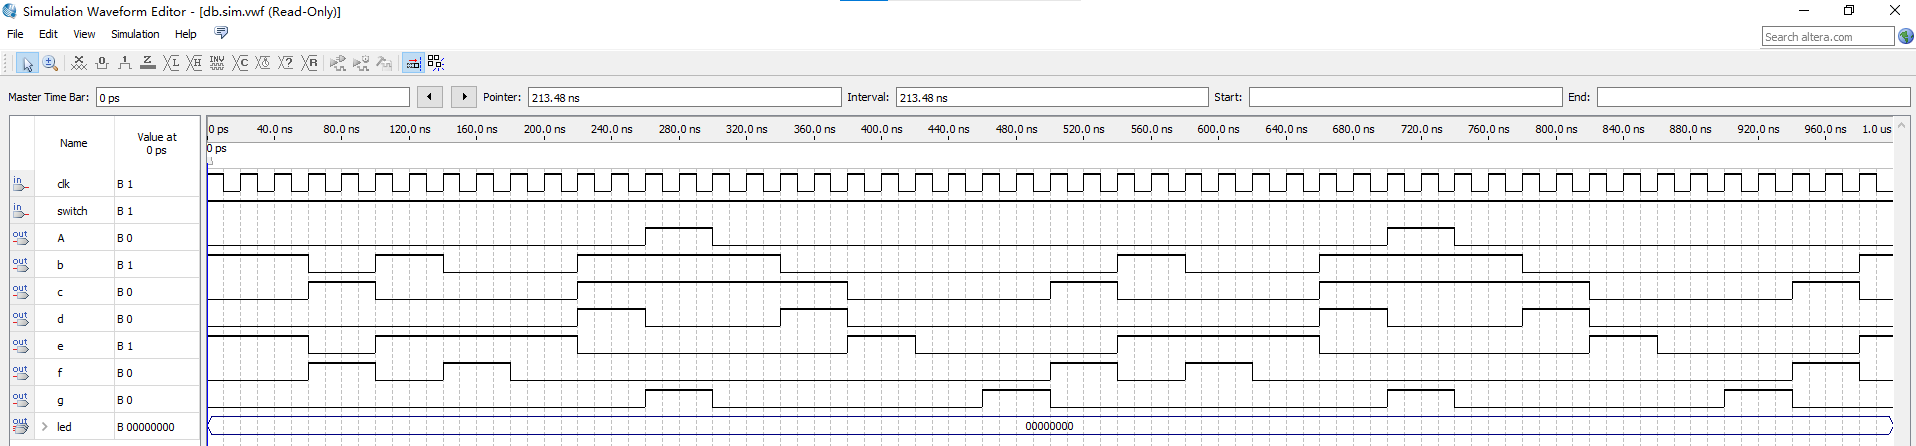
\includegraphics[width=0.75\textwidth]{任务2仿真.png}
    \caption{switch = 1 时的学号序列模式功能仿真波形}
    \label{e5:fig:sim2}
\end{figure}

\texttt{switch} 一直保持高电平，系统处于学号序列输出模式。\texttt{time2} 的地址从 0 递增到 10 再归零循环，七段输出 \texttt{A,b,c,d,e,f,g} 随之变化，依次给出 \texttt{2539FLEP980} 各字符对应的段选码。例如地址为 0 时 \texttt{A,b,c,d,e,f,g} 为 \texttt{0100100}，对应字符 \texttt{2}，与表~\ref{e5:tab:xuehaomif} 的映射完全一致。这时正弦波通路被关闭，\texttt{led[7..0]} 保持 \texttt{00000000} 不变。可见学号 ROM 的扫描和译码显示功能都正确。

\subsection{引脚分配与下载验证}

打开 Pin Planner，把各端口锁定到 DE0 开发板对应的硬件资源上，分配关系见表~\ref{e5:tab:pins}。

\begin{table}[H]
    \centering
    \caption{引脚分配：端口与 DE0 板载资源的对应关系}
    \label{e5:tab:pins}
    \begin{tabular}{ccl}
        \toprule
        \textbf{端口} & \textbf{方向} & \textbf{对应 DE0 硬件资源} \\
        \midrule
        clk               & 输入 & 板载 50\,MHz 系统时钟 CLOCK \\
        switch            & 输入 & 模式选择拨码开关 \\
        led[7..0]         & 输出 & 8 个红色 LED，LEDR7$\sim$LEDR0 \\
        A, b, c, d, e, f, g & 输出 & 七段数码管 HEX0 的 a$\sim$g 段 \\
        \bottomrule
    \end{tabular}
\end{table}

重新编译后，接上 USB-Blaster，用 JTAG 模式把 \texttt{.sof} 配置文件下载到 DE0 开发板进行硬件验证：

\begin{itemize}
    \item \texttt{switch} 拨到低电平时，系统进入正弦波模式，8 位 LED 以约 1\,Hz 的节奏依次刷新，亮灭组合呈现正弦幅值先增大后减小的周期变化，数码管显示保持不变。
    \item \texttt{switch} 拨到高电平时，系统进入学号序列模式，七段数码管 HEX0 以约 1\,Hz 的节奏循环显示 \texttt{2}、\texttt{5}、\texttt{3}、\texttt{9}、\texttt{F}、\texttt{L}、\texttt{E}、\texttt{P}、\texttt{9}、\texttt{8}、\texttt{0} 共 11 个字符，LED 全部熄灭。
    \item 拨动 \texttt{switch} 可在两种模式间实时切换，运行稳定，硬件现象与仿真一致。
\end{itemize}

\section{实验过程中的问题}

\begin{enumerate}
    \item \textbf{ROM 数据宽度的选择}。学号字符 ROM 第一次配置时数据宽度设大了，其实 11 个字符的编码索引只到 10，用 4 位就够。位宽偏大不影响功能，但多占了存储资源。后来用 MegaWizard 把数据宽度改成 4 位、深度取 32 字，占用就合理了。
    \item \textbf{\texttt{.mif} 文件要与 ROM 参数对上}。\texttt{.mif} 里的 \texttt{WIDTH}、\texttt{DEPTH} 必须与 ROM IP 的位宽、深度一致，地址和数据的基数 \texttt{ADDRESS\_RADIX}、\texttt{DATA\_RADIX} 也要写对，否则综合时会报错，提示初始化数据无法识别。正弦采样的 \texttt{.mif} 用 \texttt{WaveToMif} 工具从波形直接生成，省去了手工填写 512 个数据，也避免了填错。
    \item \textbf{仿真时间过长}。实际分频系数很大，分到 1\,Hz 要对 50\,MHz 计数 2500 万次，计数器跑完一整轮 ROM 扫描需要很久，仿真效率很低。办法是仿真时先把分频比调小，让计数器快速走完地址，短时间内就能验证逻辑；下载前再把分频比改回去，保证实际输出约 1\,Hz。
    \item \textbf{模式切换的实现方式}。要求 3 要两种模式能用开关切换。本设计没有在 ROM 的数据输出端做多路选择，而是用 \texttt{switch} 经反相器和与门门控两条通路的扫描时钟，只让选中那条的计数器走时钟、另一条冻结。这样实现简单，两条通路互不干扰；被冻结通路的 ROM 寄存输出保持原值，例如正弦通路停下时 LED 就保持在初始的 0。
\end{enumerate}

\section{心得体会}

\begin{enumerate}
    \item 这次实验让我把 ROM 在 FPGA 中的用法理解得更清楚。ROM 就是一张查找表，配上地址计数器顺序扫描，就能产生任意波形、循环显示字符序列。先把数据存好、再按地址取出来，DDS 这类技术依靠的正是这个思路。
    \item 配置 \texttt{altsyncram} ROM IP 核、编写 \texttt{.mif} 初始化文件的过程，让我熟悉了 MegaWizard 的用法和存储器初始化的格式要求。用 IP 核可以直接调用 FPGA 内部的专用存储块，比用逻辑单元搭建存储器更省资源。
    \item 这个系统里分频器、计数器、ROM、译码器和门电路都用上了，做法是 VHDL 文本与 BDF 原理图配合：模块内部的逻辑用 VHDL 描述更方便，模块之间怎么连、信号往哪走用原理图看得更清楚。把正弦波和学号两条通路设计出来、再用门控切换，我对多模块数字系统从设计到仿真、再到下载验证的整个流程也熟悉了不少。
\end{enumerate}

% ==================== 实验6：基于 FPGA 的信号发生器 ====================
\graphicspath{{../6. adda/figures/}}
\chapter{基于 FPGA 的信号发生器}

\section{实验目的}

\begin{enumerate}
    \item 掌握直接数字频率合成 DDS 的查表式波形发生原理，理解用计数器扫描 ROM 地址、把预存采样按顺序读出来重建波形的方法。
    \item 学会用 Quartus II 的 PLL IP 核对板载时钟倍频，掌握用 \texttt{altsyncram} ROM IP 核和 \texttt{.mif} 文件存储波形数据的流程。
    \item 学会用 VHDL 编写地址计数器和数据选择器，再用原理图把 PLL、计数器、ROM、数据选择器连成完整系统，完成文本设计与原理图设计的混合开发。
    \item 理解 8 位 DA 模块 AD9708 把数字码转换为模拟电压的原理，能用拨码开关切换输出波形并用示波器观测验证。
\end{enumerate}

\section{实验要求}

本次实验的要求以现场给出的实验内容为准，具体如下：

\begin{enumerate}
    \item \textbf{要求 1}：配置一块宽度为 8 位的 ROM，在 ROM 中存储 256 个地址的正弦波数据。用 PLL 生成 100\,MHz 时钟作为计数器的计数脉冲，计数器的输出作为地址去读取 ROM 的内容，再把正弦波信号通过 DA 模块 AD9708 转换成模拟信号，通过示波器显示波形。
    \item \textbf{要求 2}：利用控制开关控制波形切换。例如拨动开关置为 0 时输出正弦波，置为 1 时输出其他波形。提示可以用 VHDL 语言写一个数据选择器。
\end{enumerate}

本组在满足要求的基础上做了扩展：一共预存正弦波、三角波、方波和斜坡波四种波形，用 A 和 C 两个拨码开关组成 2 位选择信号，通过 VHDL 写的数据选择器在四种波形之间切换。当 A 与 C 都置 0 时输出正弦波，其余三种组合分别输出另外三种波形。

\section{实验设备}

\begin{itemize}
    \item Quartus II 开发软件，含 MegaWizard Plug-In Manager、PLL IP 核和 ROM IP 核
    \item DE0 开发板，FPGA 型号为 Cyclone V \texttt{5CEBA4F23C7}
    \item USB-Blaster 下载线及计算机
    \item AD9708 高速 8 位 DA 转换子板
    \item RIGOL DHO1204 数字示波器
    \item 板载 50\,MHz 晶振、两个波形选择拨码开关 A 与 C
\end{itemize}

\section{实验原理}

\subsection{DDS 查表式波形发生原理}

直接数字频率合成 DDS 的核心思想是查表：先把一个完整周期的波形按等间隔采样，量化成数字码预存进 ROM；工作时用一个地址计数器在高速时钟驱动下从 0 扫到最大地址再归零，ROM 就按存储顺序循环送出各个采样点，存进去的波形在输出端被逐点重建出来。ROM 只完成地址到数据的映射
\[
    \mathrm{data\_out} = \mathrm{ROM}[\mathrm{addr}],
\]
真正让数据随时间自动输出的是不断累加的地址计数器。

本实验的 ROM 用 Quartus II 的 \texttt{altsyncram} IP 核实现，数据宽度 8 位、存储深度 256 字、地址位宽 8 位，对应 $2^8 = 256$ 个地址。地址计数器 \texttt{Vhdl1} 是一个 8 位模 256 计数器，每来一个时钟上升沿加 1，计满 255 后归零，正好循环扫完 ROM 的 256 个单元，把一个周期的波形重复输出。

\subsection{PLL 倍频与输出波形频率}

DE0 开发板的板载系统时钟为 50\,MHz，要求用 100\,MHz 作为计数脉冲，因此用 PLL IP 核把参考时钟倍频一倍。PLL 以板载 50\,MHz 为参考时钟 \texttt{refclk}，输出 \texttt{outclk\_0} 为 100\,MHz，作为所有计数器和 ROM 的公共时钟。

计数器每 256 个时钟扫完一个周期的波形，所以输出波形的频率为
\[
    f_{\text{out}} = \frac{f_{\text{clk}}}{256} = \frac{100\,\text{MHz}}{256} \approx 390.6\,\text{kHz}.
\]
这就是示波器上观测到的波形重复频率。

\subsection{四种波形的 ROM 数据}

四块 ROM 分别用四个 \texttt{.mif} 文件初始化，每个文件存一个周期对应波形的 256 点 8 位采样，数值范围 $0\sim255$。各波形在几个关键地址上的采样值见表~\ref{e6:tab:wavedata}，由此可以看出它们的形状。

\begin{table}[H]
    \centering
    \caption{四块 ROM 初始化文件与对应波形的特征采样值}
    \label{e6:tab:wavedata}
    \small
    \begin{tabular}{lccccl}
        \toprule
        \textbf{初始化文件} & \textbf{地址 0} & \textbf{地址 64} & \textbf{地址 128} & \textbf{地址 192} & \textbf{波形} \\
        \midrule
        \texttt{dds\_256x8b\_wave.mif}  & 127 & 254 & 127 & 0   & 正弦波 \\
        \texttt{dds\_256x8b\_wave1.mif} & 0   & 128 & 255 & 128 & 三角波 \\
        \texttt{dds\_256x8b\_wave3.mif} & 255 & 255 & 0   & 0   & 方波 \\
        \texttt{dds\_256x8b\_wave4.mif} & 0   & 64  & 128 & 192 & 斜坡波 \\
        \bottomrule
    \end{tabular}
\end{table}

正弦波从中点 127 起，在地址 64 升到峰值 254，地址 128 回到中点，地址 192 降到谷底 0，呈完整正弦变化；三角波从 0 线性升到地址 128 的峰值 255 再线性降回；方波在前半周期保持 255、后半周期保持 0；斜坡波随地址线性递增，从 0 一直到 255。

\subsection{数据选择器与波形切换}

要让一套硬件输出多种波形，关键是在四块 ROM 的输出之间做选择。本实验用 VHDL 写了一个数据选择器 \texttt{bus\_mux}，它有四路 8 位输入总线 \texttt{bus0}$\sim$\texttt{bus3} 和两个选择端 \texttt{sel0}、\texttt{sel1}，根据 \texttt{sel1 sel0} 的组合把其中一路接到 8 位输出 \texttt{dout}。顶层把拨码开关 A 接到 \texttt{sel1}、C 接到 \texttt{sel0}，于是 A 和 C 的四种组合对应四种波形，逻辑见表~\ref{e6:tab:mux}。

\begin{table}[H]
    \centering
    \caption{数据选择器开关组合与输出波形对照}
    \label{e6:tab:mux}
    \begin{tabular}{cccccl}
        \toprule
        \textbf{A (sel1)} & \textbf{C (sel0)} & \textbf{选通总线} & \textbf{数据来源} & \textbf{初始化文件} & \textbf{输出波形} \\
        \midrule
        0 & 0 & \texttt{bus0} & ROM1 & \texttt{dds\_256x8b\_wave.mif}  & 正弦波 \\
        0 & 1 & \texttt{bus1} & ROM2 & \texttt{dds\_256x8b\_wave1.mif} & 三角波 \\
        1 & 0 & \texttt{bus2} & ROM3 & \texttt{dds\_256x8b\_wave3.mif} & 方波 \\
        1 & 1 & \texttt{bus3} & ROM4 & \texttt{dds\_256x8b\_wave4.mif} & 斜坡波 \\
        \bottomrule
    \end{tabular}
\end{table}

四块 ROM 各配一个地址计数器，全部接同一路 100\,MHz 时钟并同步计数，所以它们时刻输出相同地址、各自读出本通路的波形采样，数据选择器只是把被选中的那一路送到输出，切换开关即可在不停机的情况下实时换波形。

\subsection{DA 转换原理}

ROM 输出的是 8 位数字码，要在示波器上看到模拟波形还需要数模转换。AD9708 是一片高速 8 位 DA 转换器，它把输入的 8 位二进制码按比例转换成模拟电流并经外围电路变成电压，输出电压与数字码近似成正比
\[
    V_{\text{out}} \approx \frac{D}{2^{8}} \, V_{\text{ref}},
\]
其中 $D$ 为输入的数字码、$V_{\text{ref}}$ 为满量程参考。计数器每个时钟更新一个 ROM 采样，AD9708 就对应输出一个电压台阶，256 个台阶连起来就重建出一个周期的模拟波形，台阶经示波器带宽平滑后即为光滑的波形曲线。

\section{实验内容}

本系统把 VHDL 文本设计和原理图设计结合起来：地址计数器和数据选择器用 VHDL 编写，PLL 和 ROM 用 IP 核生成，编译后各自生成原理图符号，再在顶层原理图中调用并连线，拼成完整系统。整个软件流程是建立工程，配置 PLL 和四块 ROM IP 核，编写各模块 VHDL 代码并生成符号，绘制顶层原理图，编译，引脚分配，下载到开发板，最后接 DA 模块和示波器观测。

\subsection{建立工程与配置 IP 核}

打开 Quartus II，用 \textbf{File $\rightarrow$ New Project Wizard} 新建工程，器件选 DE0 开发板对应的 Cyclone V \texttt{5CEBA4F23C7}。随后配置两类 IP 核：

\begin{enumerate}
    \item \textbf{PLL IP 核}：用 MegaWizard 生成一个锁相环，参考时钟频率设为 50\,MHz，输出 \texttt{outclk\_0} 设为 100\,MHz，把板载时钟倍频一倍后作为全局计数脉冲。
    \item \textbf{四块 ROM IP 核}：按 \texttt{ROM: 1-PORT} 类型各配一块，输出位宽都设为 8 位、深度都设为 256 字、地址 8 位，并分别勾选用 \texttt{.mif} 文件初始化，依次指定 \texttt{dds\_256x8b\_wave.mif}、\texttt{dds\_256x8b\_wave1.mif}、\texttt{dds\_256x8b\_wave3.mif}、\texttt{dds\_256x8b\_wave4.mif}。这四个 \texttt{.mif} 里的采样值不是手工填的，而是用波形转 MIF 上位机软件从一个周期的目标波形生成，幅值范围 $0\sim255$。正弦波 \texttt{.mif} 的前几个采样值列在表~\ref{e6:tab:sinmif}。
\end{enumerate}

\begin{table}[H]
    \centering
    \caption{正弦波 ROM 初始化文件 \texttt{dds\_256x8b\_wave.mif} 部分采样值}
    \label{e6:tab:sinmif}
    \begin{tabular}{ccccccccc}
        \toprule
        地址 & 0 & 1 & 2 & 3 & 4 & 5 & 6 & 7 \\
        \midrule
        十进制数据 & 127 & 130 & 133 & 136 & 139 & 142 & 145 & 148 \\
        \bottomrule
    \end{tabular}
\end{table}

\subsection{编写 VHDL 子模块}

\subsubsection{8 位地址计数器 Vhdl1}

\texttt{Vhdl1} 负责产生 ROM 的 8 位地址。计数脉冲每来一个上升沿就加 1，数到 255 后归零并给出一个进位脉冲 \texttt{COUT}，这样循环扫完 256 个地址；复位端 \texttt{RST} 低电平有效，顶层把它接到 VCC，让计数器始终不复位、保持正常计数。

\begin{minted}{vhdl}
LIBRARY IEEE;
USE IEEE.STD_LOGIC_1164.ALL;
USE IEEE.STD_LOGIC_UNSIGNED.ALL;
ENTITY Vhdl1 IS
    PORT ( clk,RST : IN  STD_LOGIC;
           DOUT    : OUT STD_LOGIC_VECTOR (7 DOWNTO 0);  -- 8位计数
           COUT    : OUT STD_LOGIC);                      -- 进位位
END Vhdl1;
ARCHITECTURE fwm OF Vhdl1 IS
    SIGNAL Q1 : STD_LOGIC_VECTOR (7 DOWNTO 0);
BEGIN
    PROCESS(clk,RST)
    BEGIN
        IF RST = '0' THEN
            Q1 <= (OTHERS => '0'); COUT <= '0';
        ELSIF clk'EVENT AND clk = '1' THEN
            Q1 <= Q1 + 1;
            COUT <= '0';
            IF Q1 >= "11111111" THEN          -- 计满 255 归零
                Q1 <= (OTHERS => '0'); COUT <= '1';
            END IF;
        END IF;
    END PROCESS;
    DOUT <= Q1;
END fwm;
\end{minted}
\captionof{listing}{8 位地址计数器 Vhdl1.vhd}
\label{e6:lst:vhdl1}

\subsubsection{四选一数据选择器 bus\_mux}

\texttt{bus\_mux} 接收四块 ROM 的 8 位输出 \texttt{bus0}$\sim$\texttt{bus3} 和两个选择端 \texttt{sel0}、\texttt{sel1}，用一段组合逻辑根据 \texttt{sel1 sel0} 把对应通路接到输出 \texttt{dout}，实现表~\ref{e6:tab:mux} 的波形选择。

\begin{minted}{vhdl}
LIBRARY IEEE;
USE IEEE.STD_LOGIC_1164.ALL;
ENTITY bus_mux IS
PORT (
    bus0  : IN  STD_LOGIC_VECTOR(7 DOWNTO 0);   -- 4 路 8 位输入总线
    bus1  : IN  STD_LOGIC_VECTOR(7 DOWNTO 0);
    bus2  : IN  STD_LOGIC_VECTOR(7 DOWNTO 0);
    bus3  : IN  STD_LOGIC_VECTOR(7 DOWNTO 0);
    sel0  : IN  STD_LOGIC;                       -- 两个独立的选择输入
    sel1  : IN  STD_LOGIC;
    dout  : OUT STD_LOGIC_VECTOR(7 DOWNTO 0)     -- 8 位输出总线
);
END bus_mux;
ARCHITECTURE Behavioral OF bus_mux IS
BEGIN
    PROCESS(bus0, bus1, bus2, bus3, sel0, sel1)
    BEGIN
        IF    sel1 = '0' AND sel0 = '0' THEN dout <= bus0;
        ELSIF sel1 = '0' AND sel0 = '1' THEN dout <= bus1;
        ELSIF sel1 = '1' AND sel0 = '0' THEN dout <= bus2;
        ELSIF sel1 = '1' AND sel0 = '1' THEN dout <= bus3;
        ELSE  dout <= (OTHERS => '0');
        END IF;
    END PROCESS;
END Behavioral;
\end{minted}
\captionof{listing}{四选一数据选择器 bus\_mux.vhd}
\label{e6:lst:busmux}

把这两个模块和 PLL、四块 ROM 分别编译，再用 \textbf{File $\rightarrow$ Create/Update $\rightarrow$ Create Symbol Files for Current File} 各自生成 \texttt{.bsf} 符号，供顶层原理图调用。

\subsection{绘制顶层原理图}

新建一个 BDF 原理图作为顶层设计，把各模块符号放上去并按下面的关系连线，顶层原理图如图~\ref{e6:fig:top}。

\begin{itemize}
    \item 输入有三个：\texttt{clk} 接板载 50\,MHz 系统时钟，A 和 C 接两个波形选择拨码开关。
    \item PLL 以 \texttt{clk} 为参考时钟，输出 100\,MHz，并经一个 \texttt{Clk\_100MHz} 输出端引出作测试点；这路 100\,MHz 时钟同时扇出到四个计数器和四块 ROM，作为公共计数脉冲和读时钟。
    \item 四个 \texttt{Vhdl1} 计数器的 \texttt{DOUT[7..0]} 分别接 ROM1$\sim$ROM4 的 \texttt{address[7..0]}，四个计数器的 \texttt{RST} 都接 VCC，始终计数。
    \item ROM1$\sim$ROM4 的输出 \texttt{q[7..0]} 分别接 \texttt{bus\_mux} 的 \texttt{bus0}$\sim$\texttt{bus3}；A 接 \texttt{sel1}，C 接 \texttt{sel0}。
    \item \texttt{bus\_mux} 的 \texttt{dout[7..0]} 接 8 位输出总线 \texttt{a[7..0]}，再拆成输出脚 0$\sim$7 送 AD9708 的数据口 D0$\sim$D7。
\end{itemize}

\begin{figure}[htbp]
    \centering
    
\includegraphics[width=0.75\textwidth]{电路图.png}
    \caption{基于 FPGA 的信号发生器顶层原理图}
    \label{e6:fig:top}
\end{figure}

\subsection{编译、引脚分配与下载}

把 BDF 设为顶层实体完整编译一遍，再打开 Pin Planner 按表~\ref{e6:tab:pins} 把各端口锁定到 DE0 开发板和 DA 子板对应的引脚上。其中输出脚 0$\sim$7 是 8 位数据的低位到高位，依次接 AD9708 的 D0$\sim$D7。

\begin{table}[H]
    \centering
    \caption{引脚分配：端口与 DE0 板载资源及 DA 模块的对应关系}
    \label{e6:tab:pins}
    \begin{tabular}{llll}
        \toprule
        \textbf{端口} & \textbf{方向} & \textbf{引脚} & \textbf{说明} \\
        \midrule
        \texttt{clk}         & 输入 & \texttt{PIN\_M9}   & 板载 50\,MHz 系统时钟，PLL 参考时钟 \\
        A                    & 输入 & \texttt{PIN\_AB13} & 波形选择开关，接 \texttt{sel1} \\
        C                    & 输入 & \texttt{PIN\_AB12} & 波形选择开关，接 \texttt{sel0} \\
        \texttt{Clk\_100MHz} & 输出 & \texttt{PIN\_M22}  & PLL 100\,MHz 时钟测试点 \\
        0                    & 输出 & \texttt{PIN\_K17}  & DA 数据 D0 \\
        1                    & 输出 & \texttt{PIN\_L17}  & DA 数据 D1 \\
        2                    & 输出 & \texttt{PIN\_M18}  & DA 数据 D2 \\
        3                    & 输出 & \texttt{PIN\_P17}  & DA 数据 D3 \\
        4                    & 输出 & \texttt{PIN\_P19}  & DA 数据 D4 \\
        5                    & 输出 & \texttt{PIN\_N19}  & DA 数据 D5 \\
        6                    & 输出 & \texttt{PIN\_T22}  & DA 数据 D6 \\
        7                    & 输出 & \texttt{PIN\_R22}  & DA 数据 D7 \\
        \bottomrule
    \end{tabular}
\end{table}

重新编译后接上 USB-Blaster，用 JTAG 模式把 \texttt{.sof} 配置文件下载到 DE0 开发板。

\subsection{接 DA 模块与示波器观测}

把 AD9708 子板的数据口接到输出脚 0$\sim$7，子板的模拟输出经 SMA 接到 RIGOL DHO1204 示波器。逐一拨动 A 和 C 两个开关，示波器上分别观测到四种波形，结果如图~\ref{e6:fig:waves}。

\begin{figure}[htbp]
    \centering
    \begin{subfigure}{0.48\textwidth}
        \centering
        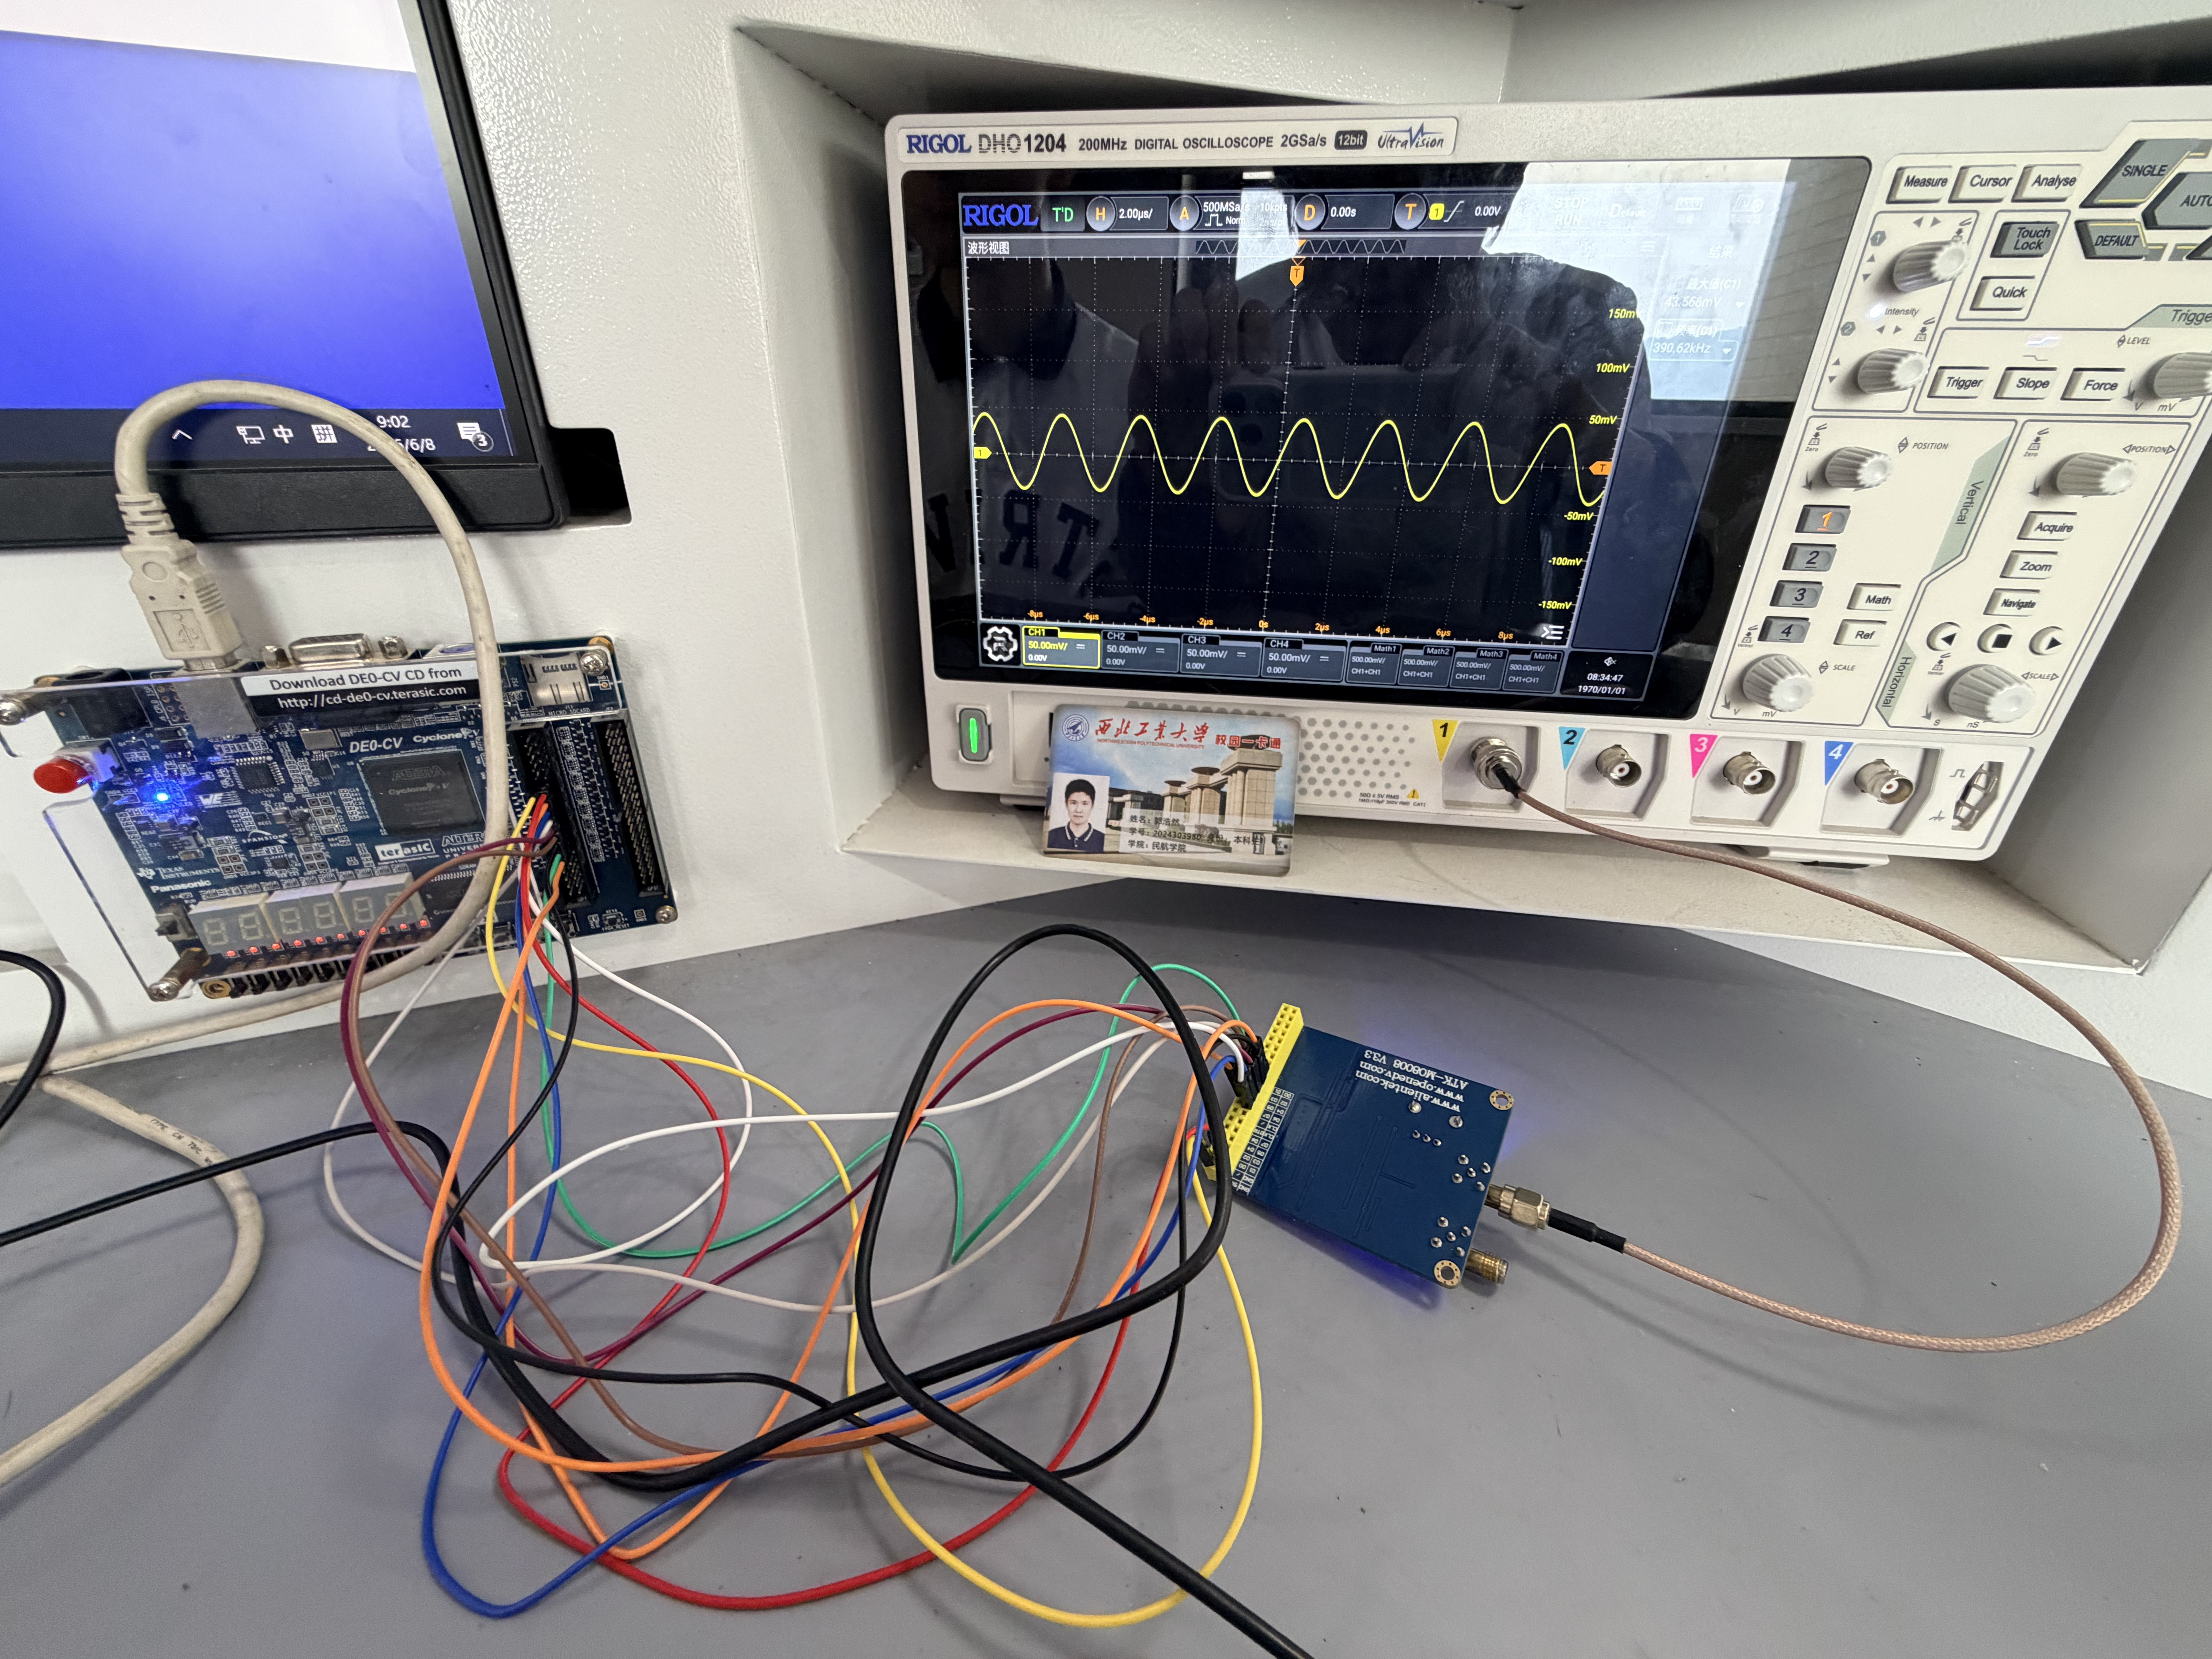
\includegraphics[width=\linewidth]{正弦波.jpg}
        \caption{正弦波输出，A = 0，C = 0}
    \end{subfigure}\hfill
    \begin{subfigure}{0.48\textwidth}
        \centering
        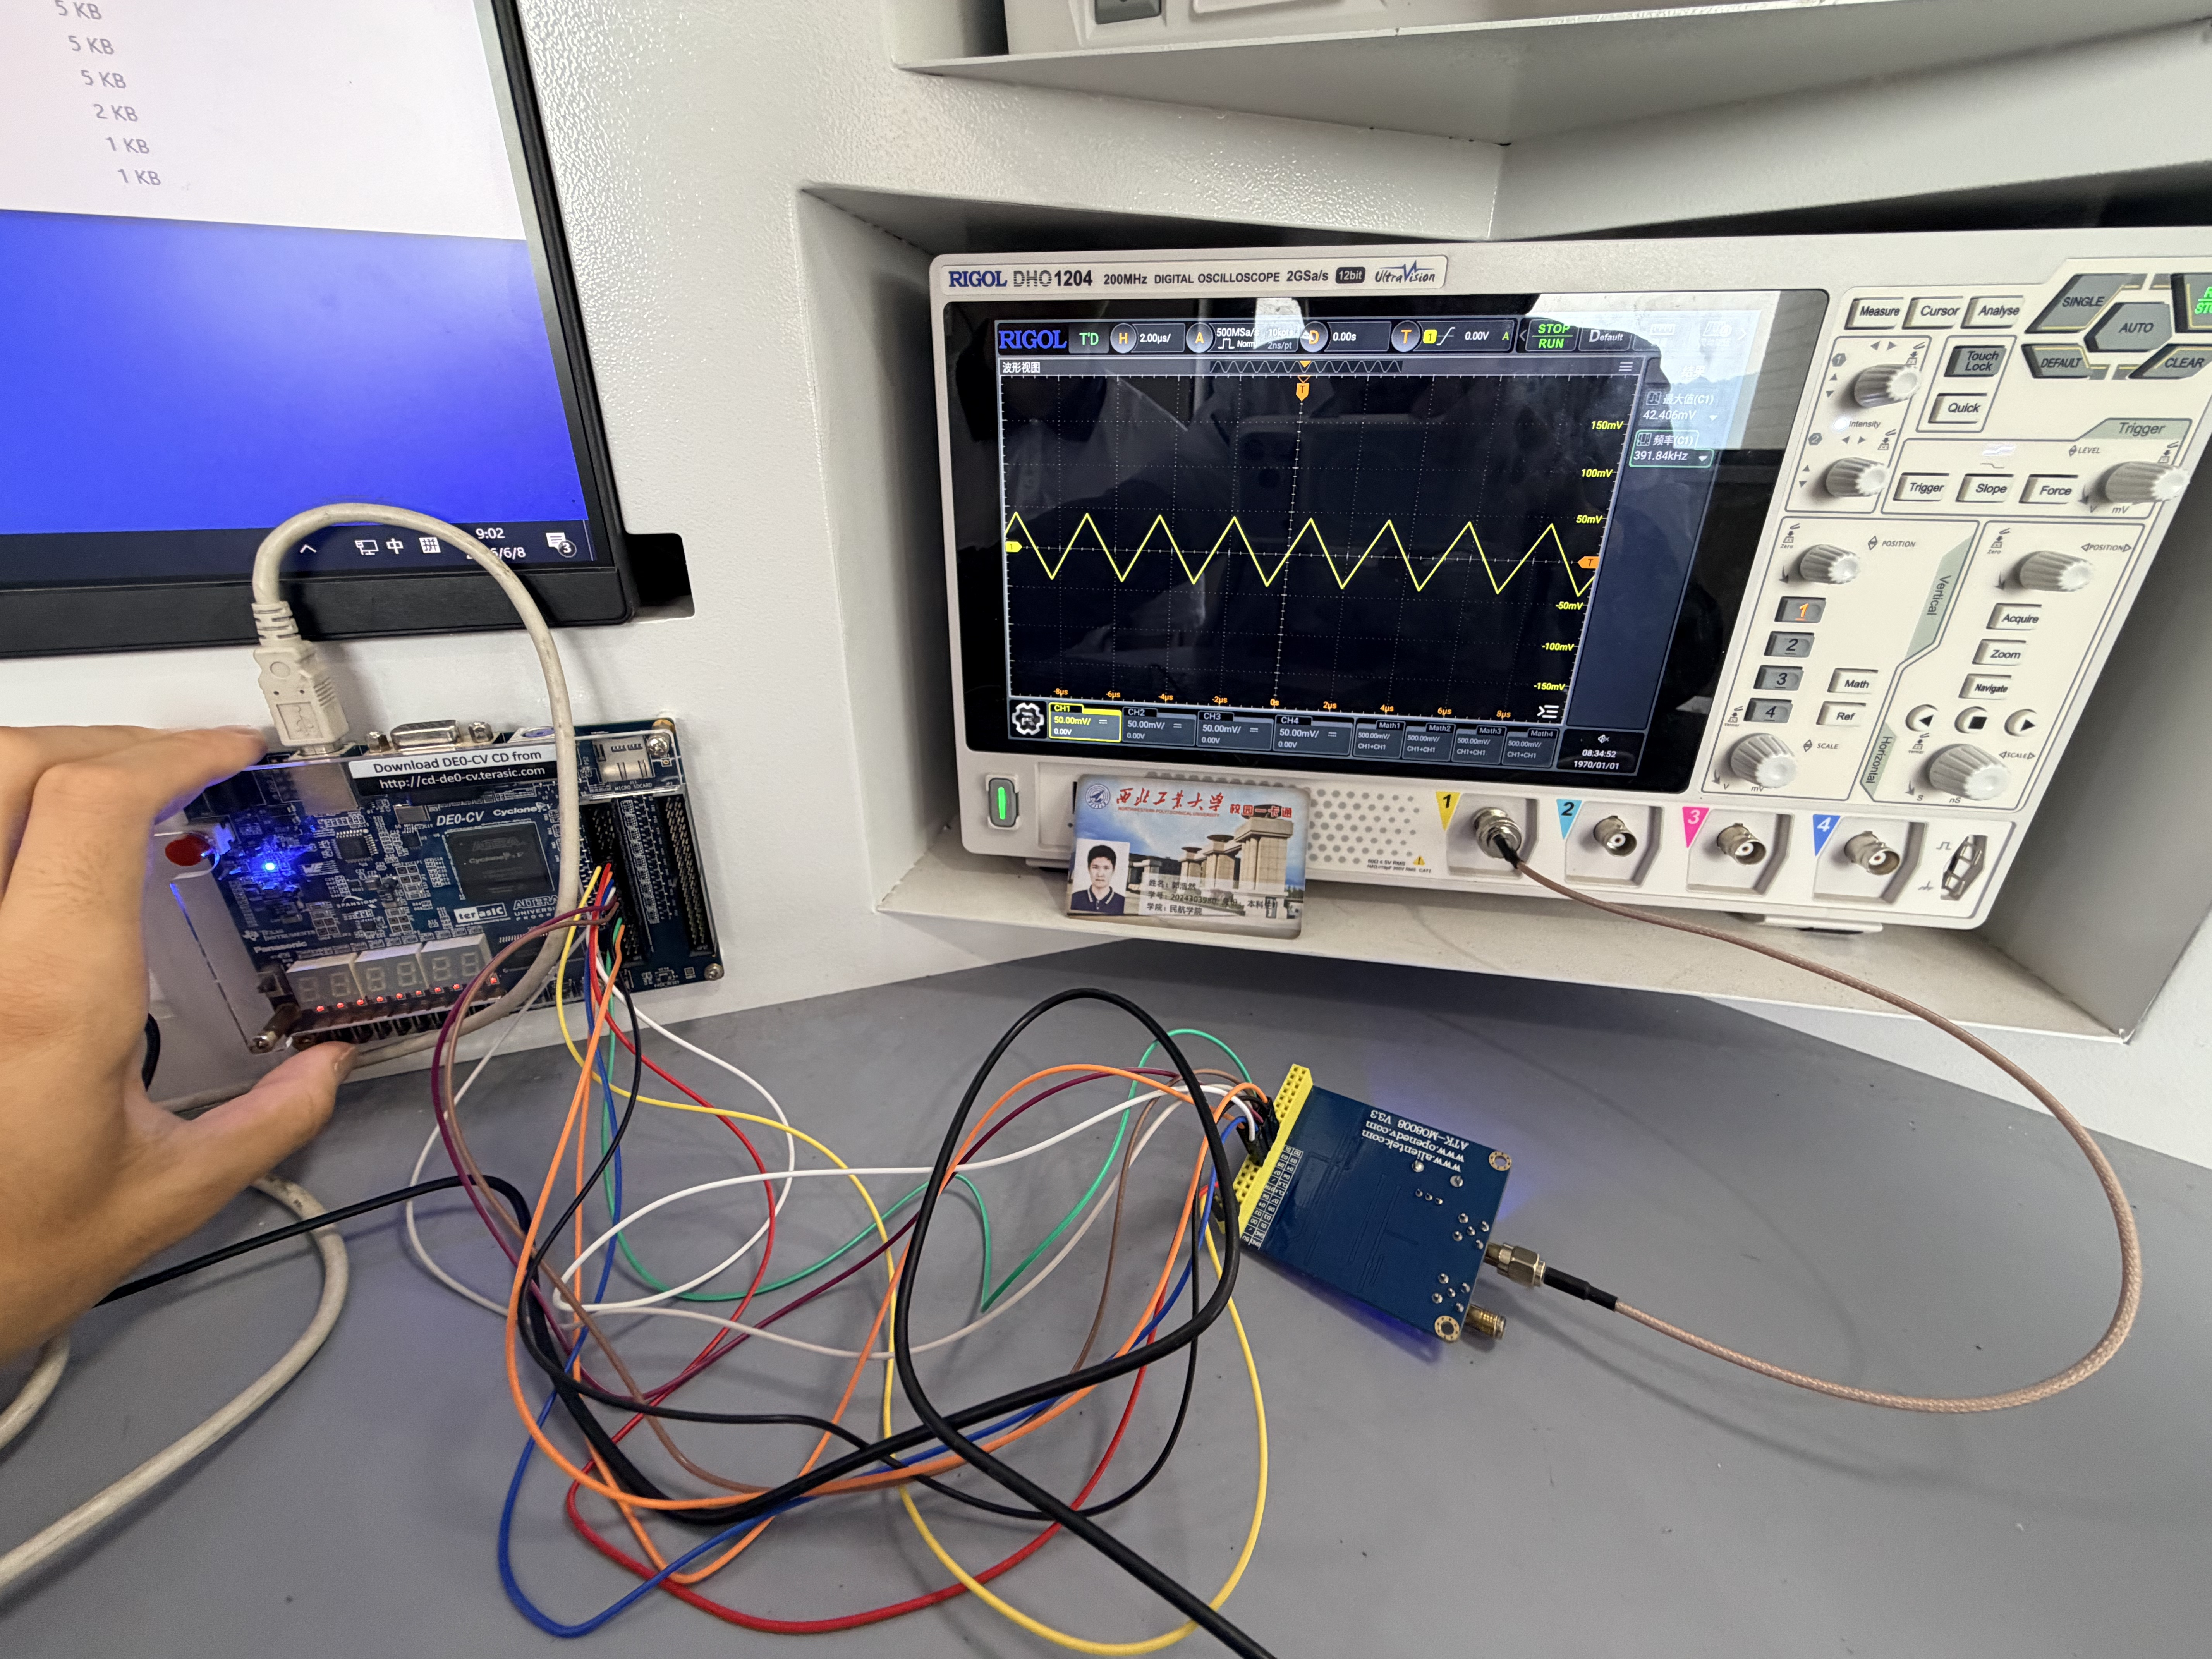
\includegraphics[width=\linewidth]{三角波.jpg}
        \caption{三角波输出，A = 0，C = 1}
    \end{subfigure}

    \vspace{6pt}
    \begin{subfigure}{0.48\textwidth}
        \centering
        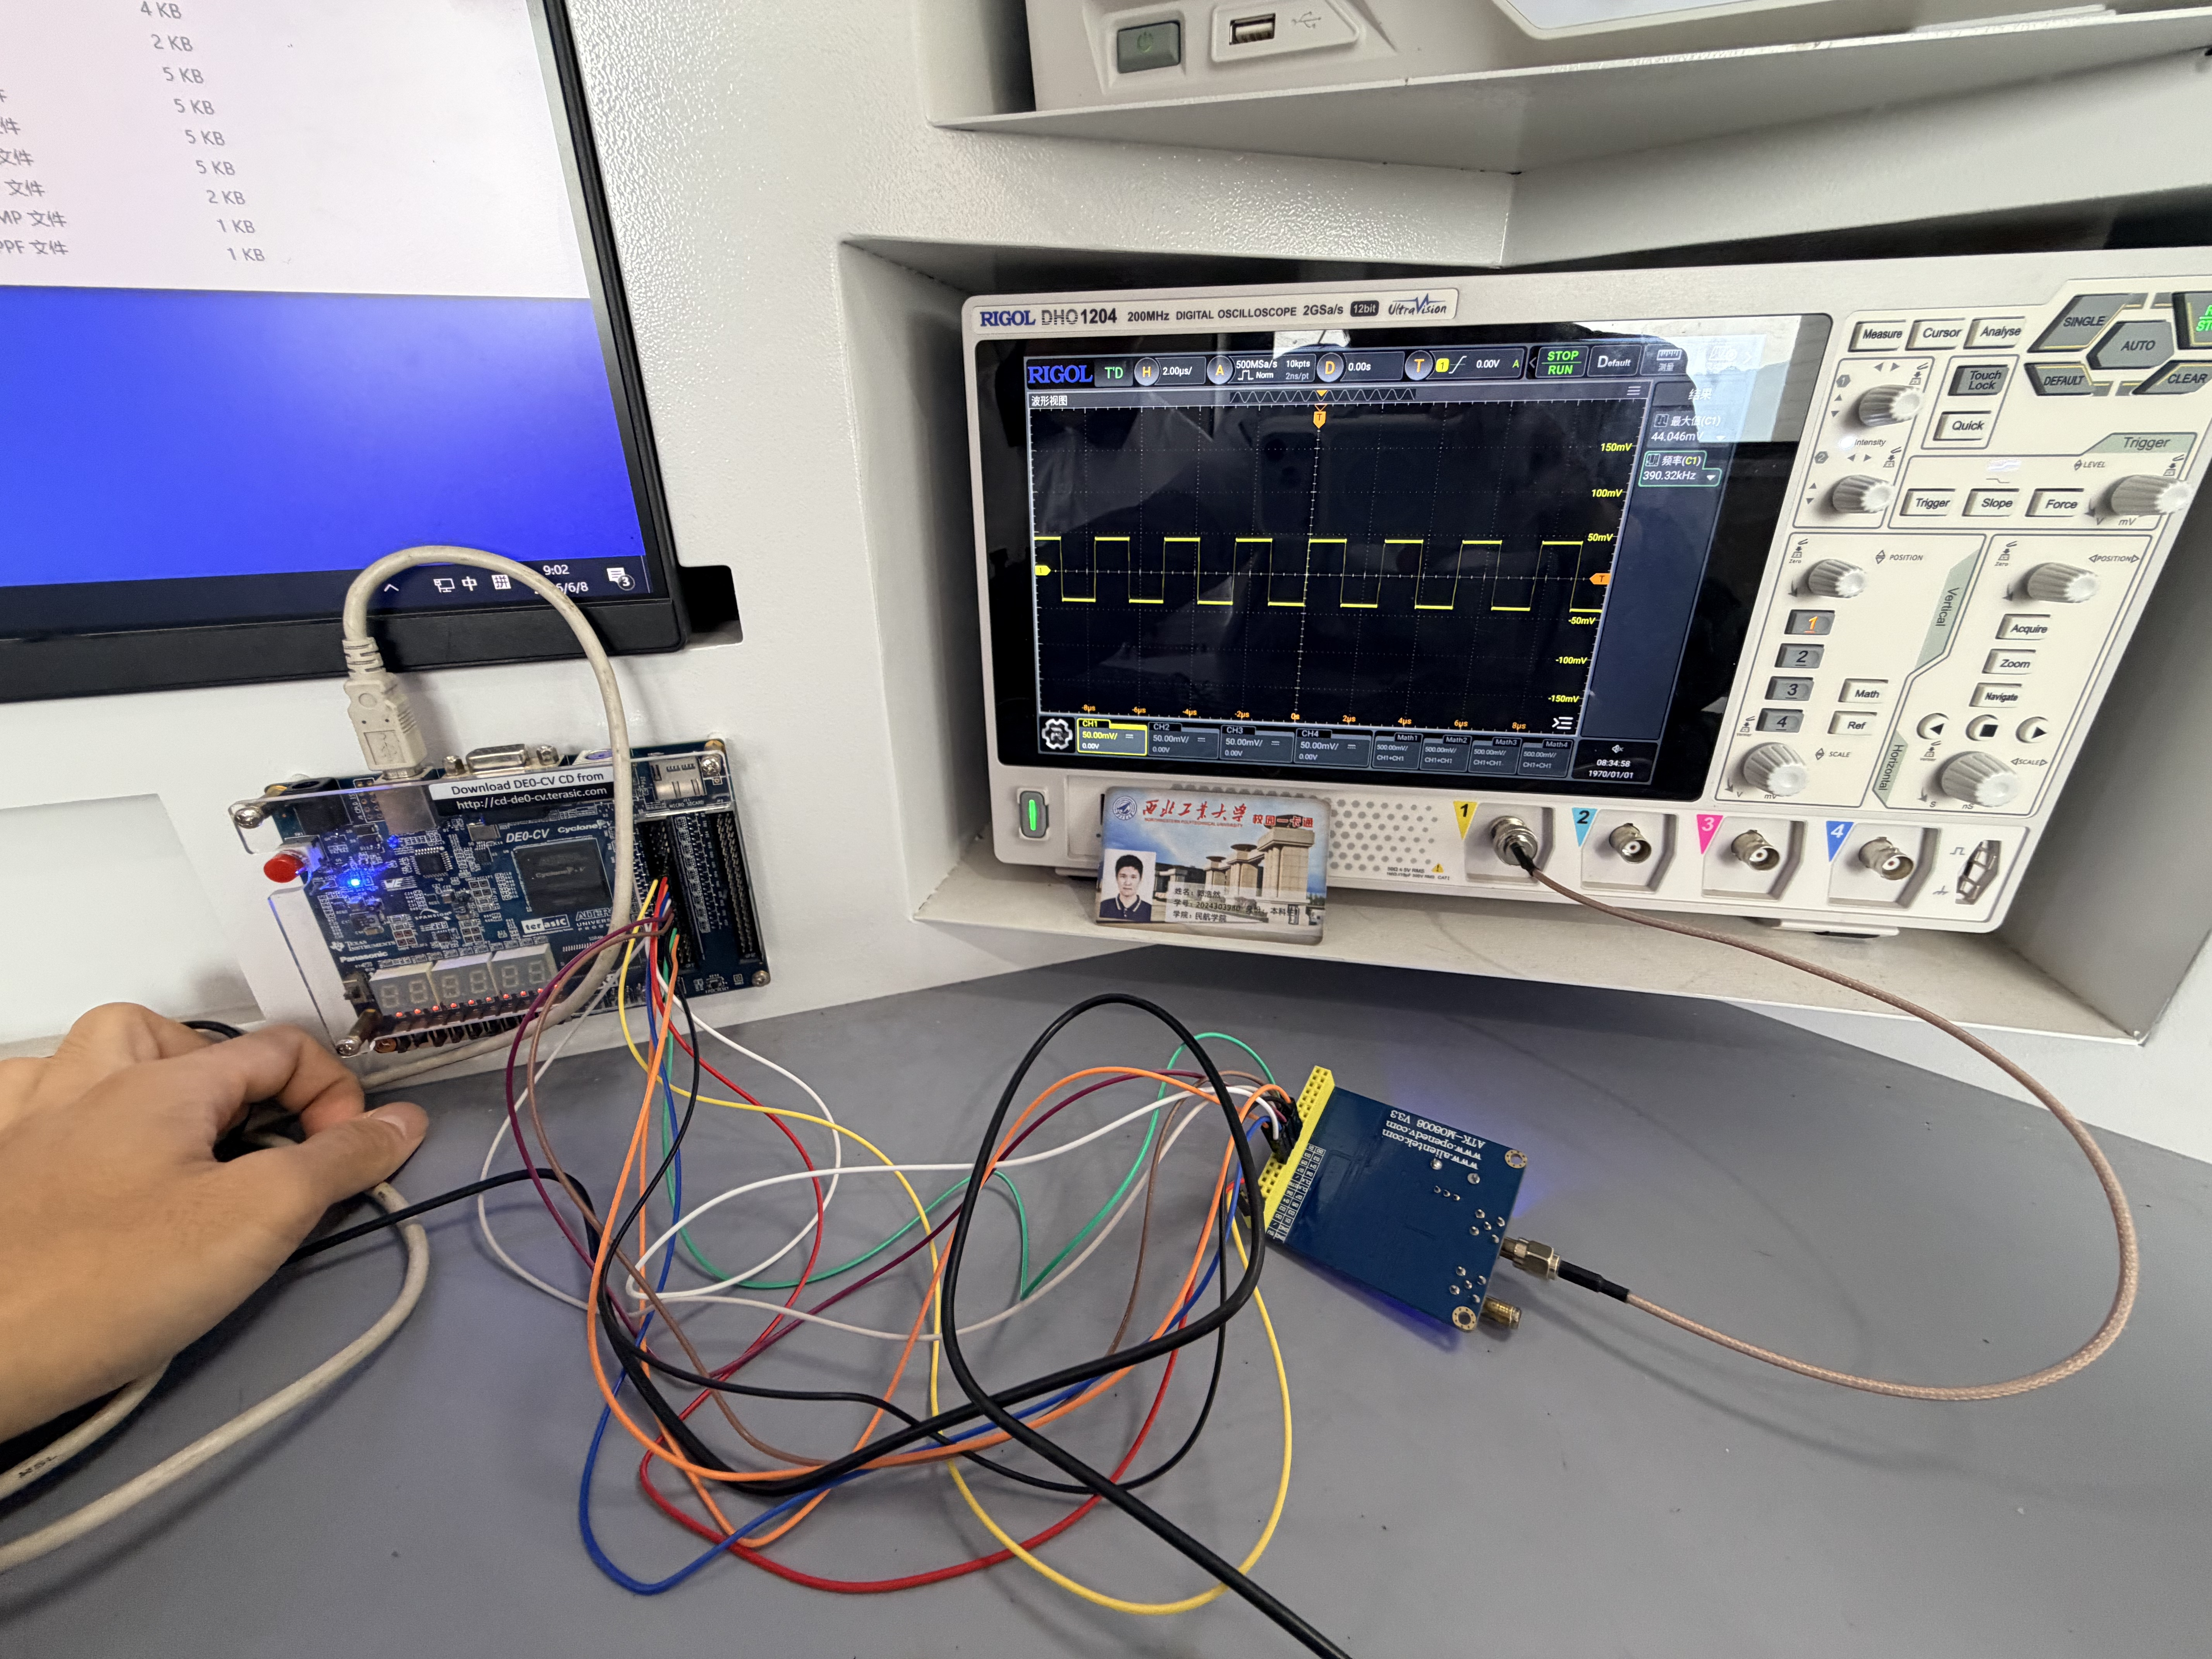
\includegraphics[width=\linewidth]{方波.jpg}
        \caption{方波输出，A = 1，C = 0}
    \end{subfigure}\hfill
    \begin{subfigure}{0.48\textwidth}
        \centering
        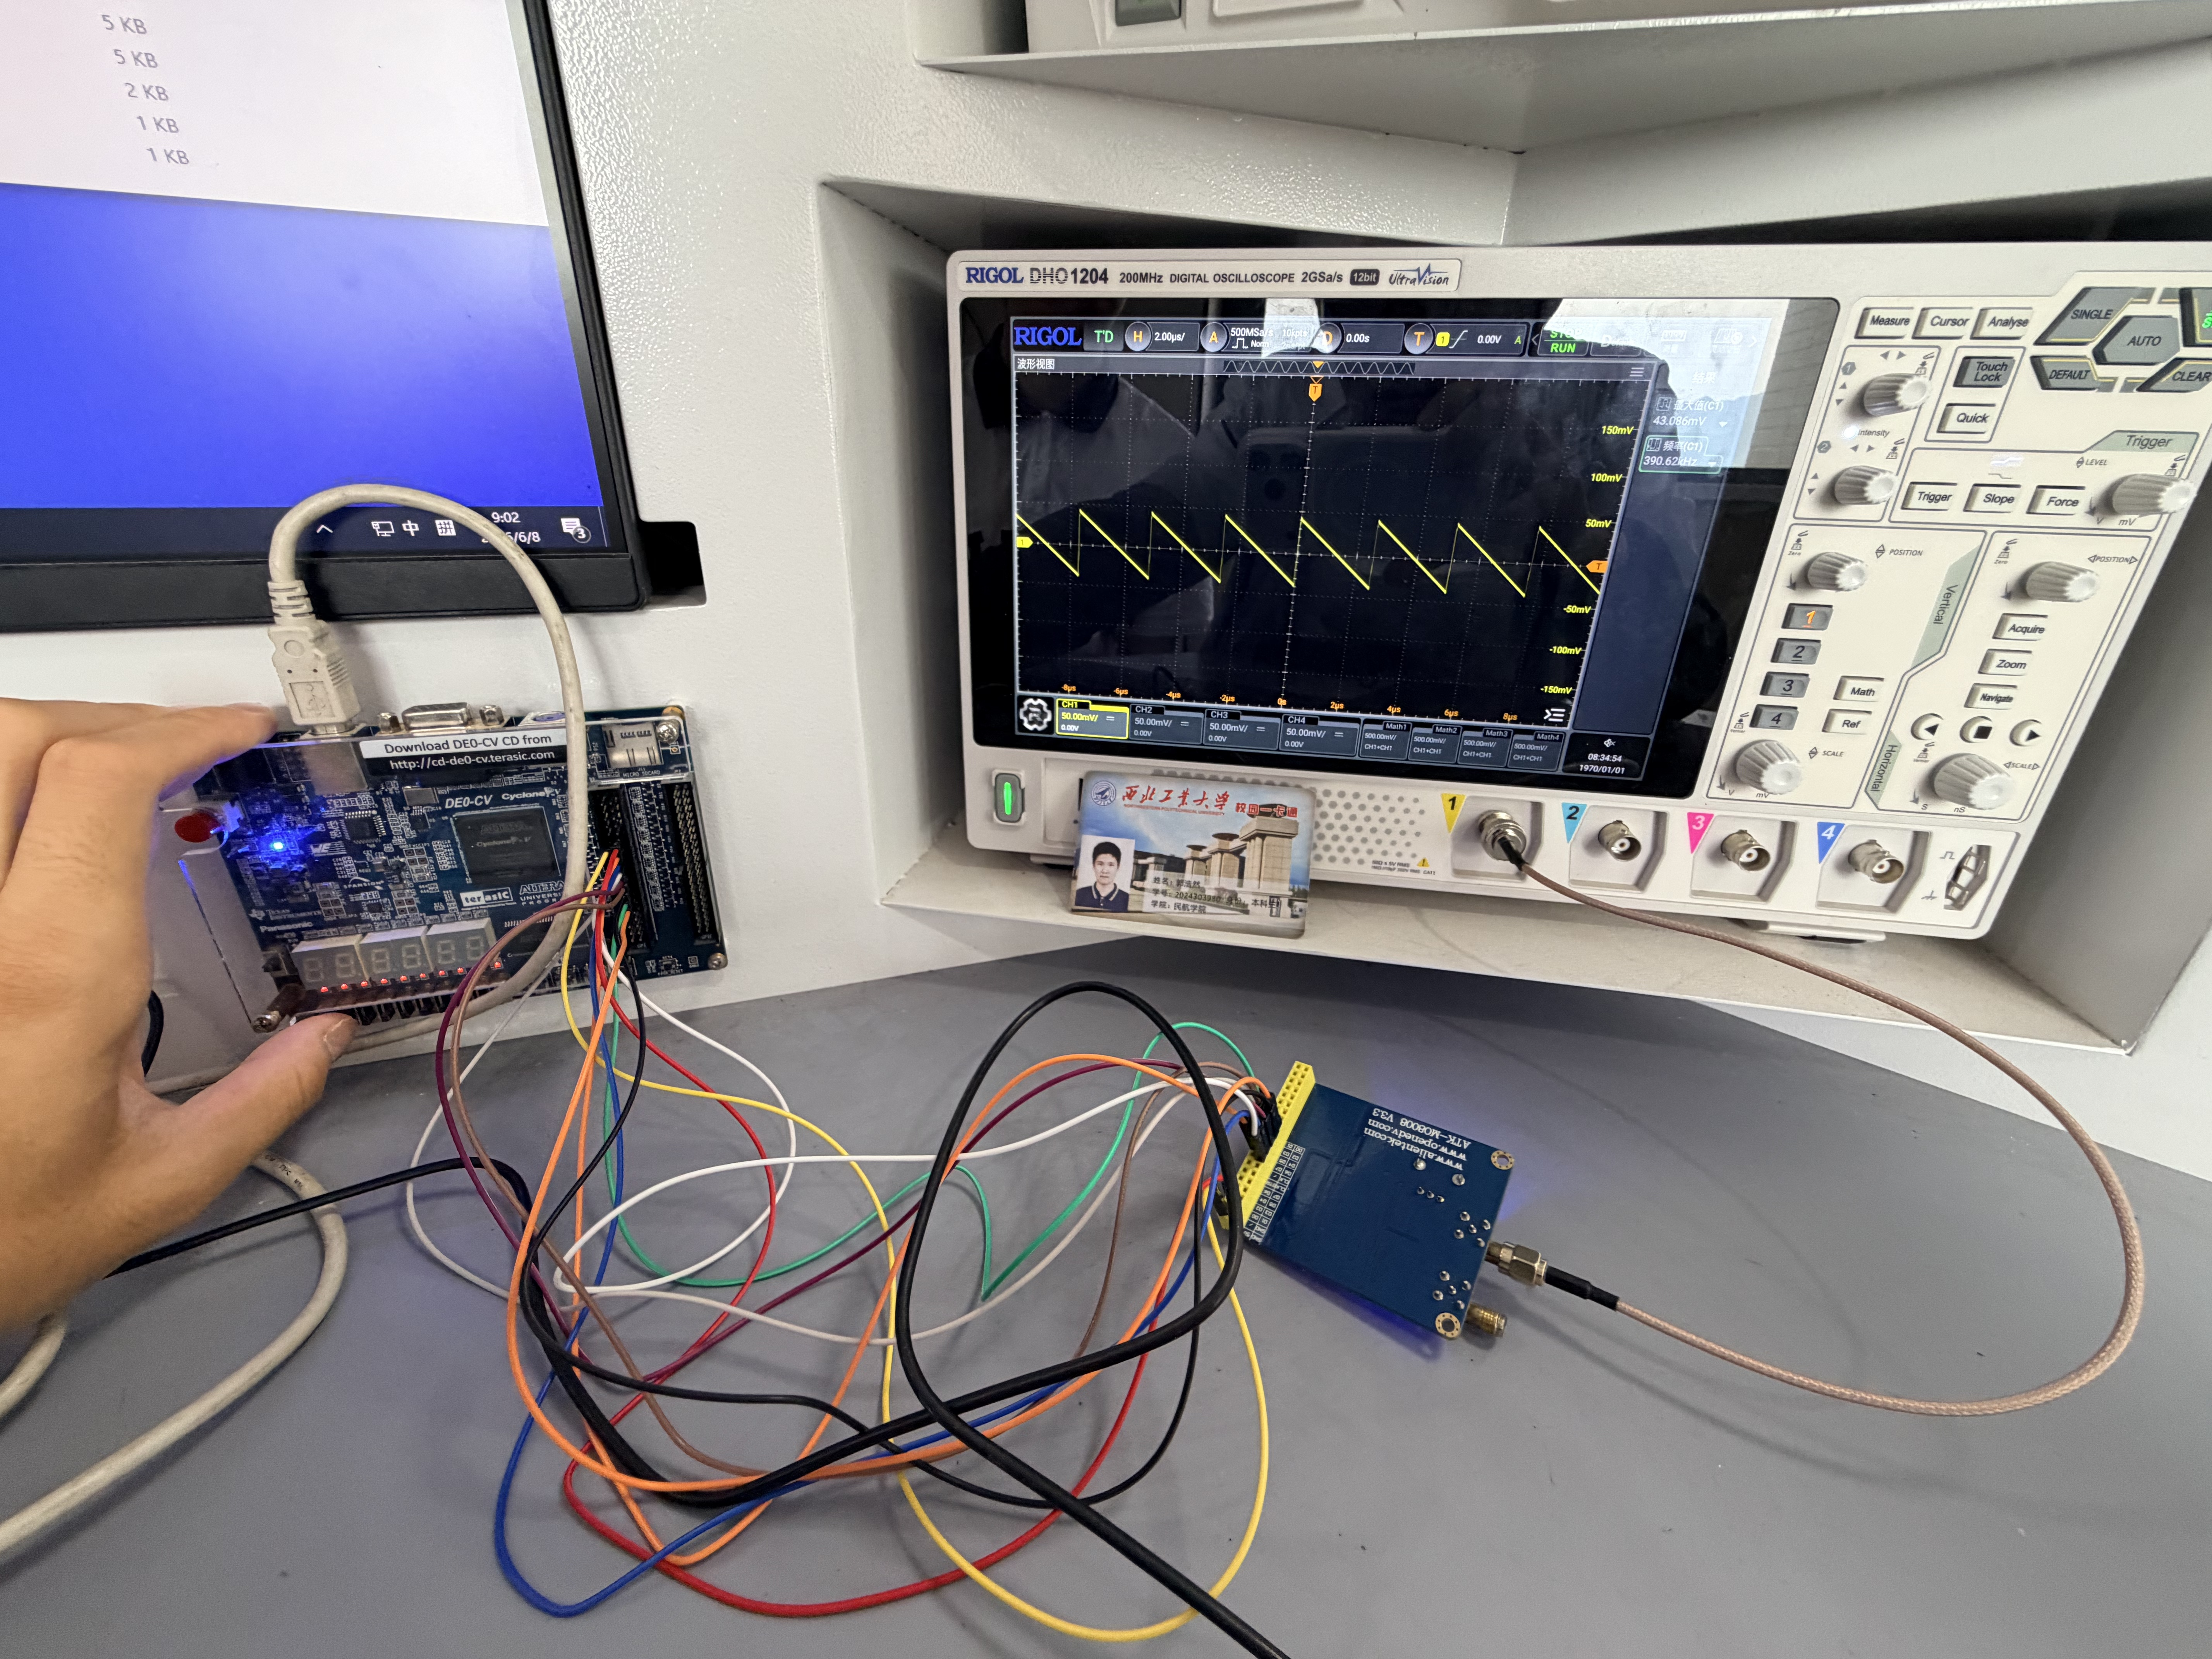
\includegraphics[width=\linewidth]{斜坡信号.jpg}
        \caption{斜坡波输出，A = 1，C = 1}
    \end{subfigure}
    \caption{四种波形的示波器实测结果}
    \label{e6:fig:waves}
\end{figure}

\subsection{数据分析}

把示波器实测波形与表~\ref{e6:tab:wavedata} 中各 ROM 预存的采样数据逐一对照，可以看出实测结果与设计完全吻合：

\begin{itemize}
    \item A 与 C 都为 0 时选通 ROM1，示波器显示一条光滑的正弦波，与 \texttt{dds\_256x8b\_wave.mif} 中从中点升到峰值再降到谷底的采样规律一致。
    \item A 为 0、C 为 1 时选通 ROM2，显示对称的三角波，对应 \texttt{dds\_256x8b\_wave1.mif} 中先线性上升到 255 再线性下降的数据。
    \item A 为 1、C 为 0 时选通 ROM3，显示方波，对应 \texttt{dds\_256x8b\_wave3.mif} 中前半周期为 255、后半周期为 0 的数据。
    \item A 为 1、C 为 1 时选通 ROM4，显示斜坡波，每个周期电压随地址线性升到满量程后迅速跌回，对应 \texttt{dds\_256x8b\_wave4.mif} 的线性递增数据。
\end{itemize}

四种波形拨动开关即可实时切换，互不干扰，验证了数据选择器和多 ROM 查表结构的正确性。波形频率约为 100\,MHz 除以 256，即 390.6\,kHz 量级，与理论计算相符。由于 DA 输出本质是 256 级电压台阶，在示波器上仔细看仍可见细小的阶梯，幅度越平缓的波形阶梯越明显，这是 8 位量化和有限采样点共同造成的，提高位宽或采样点数可以让波形更光滑。

\section{实验过程中的问题}

\begin{enumerate}
    \item \textbf{用 PLL 产生 100\,MHz 计数脉冲}。板载晶振只有 50\,MHz，要按要求得到 100\,MHz 必须借助 PLL 倍频。配置时把参考时钟设为 50\,MHz、输出设为 100\,MHz，综合后用 \texttt{Clk\_100MHz} 引出测试点确认时钟正常，再把它作为计数器和 ROM 的公共时钟。
    \item \textbf{\texttt{.mif} 文件要与 ROM 参数对上}。\texttt{.mif} 里的 \texttt{WIDTH} 和 \texttt{DEPTH} 必须与 ROM IP 的位宽 8、深度 256 一致，地址和数据的基数也要写对，否则综合时会报初始化数据无法识别的错误。四个 \texttt{.mif} 都用波形转 MIF 上位机软件从目标波形直接生成，省去手工填 256 个数据，也避免填错。
    \item \textbf{DA 数据线位序的对应}。AD9708 的数据口 D0$\sim$D7 要和输出脚 0$\sim$7 一一对应，如果高低位接反，输出波形会被镜像或失真。接线时按表~\ref{e6:tab:pins} 的对应关系逐根核对，确认低位脚接 D0、高位脚接 D7。
    \item \textbf{开关组合与波形的对应关系}。数据选择器用 A 接 \texttt{sel1}、C 接 \texttt{sel0}，刚开始容易把两个开关的高低位记混，导致切出来的波形和预期不符。对照表~\ref{e6:tab:mux} 把每种组合实测一遍，确认四种波形都能正确切换。
\end{enumerate}

\section{心得体会}

\begin{enumerate}
    \item 这次实验让我把 DDS 查表式波形发生的思路理解得更透彻。把一个周期的波形采样预存进 ROM，再用计数器顺序扫描地址，就能不断重建出任意波形，正弦波、三角波、方波、斜坡波只是换了 \texttt{.mif} 里的数据而已。这种存采样、扫地址的方法是函数信号发生器的基础。
    \item 配置 PLL 和 ROM 这两类 IP 核，让我熟悉了 MegaWizard 的用法。用 PLL 可以方便地把板载时钟倍频到需要的频率，用 ROM IP 核可以直接调用 FPGA 内部的专用存储块来存波形，比自己用逻辑搭建省资源也更可靠。
    \item 整个系统是 VHDL 文本设计与原理图设计的结合：计数器和数据选择器的逻辑用 VHDL 描述更清晰，PLL、ROM、多个模块之间怎么连用原理图看得更直观。再加上 AD9708 把数字码还原成模拟波形，我完整走通了从数字设计到数模转换、再到示波器观测的全链路，对数字系统的整体设计流程熟悉了不少。
\end{enumerate}

% ==================== 实验7：基于 FPGA 的模数转换电路 ====================
\graphicspath{{../7. adda2/figures/}}
\chapter{基于 FPGA 的模数转换电路}

\section{实验目的}

\begin{enumerate}
    \item 理解高速模数转换芯片 AD9280 的工作原理，掌握它把 $-5\,$V 至 $+5\,$V 模拟电压经衰减后转换成 0 至 255 的 8 位数字码的映射关系。
    \item 掌握用计数器对板载时钟分频的方法，理解为什么要把 50\,MHz 系统时钟分频后才能作为 AD9280 的驱动时钟。
    \item 学会用 VHDL 编写显示译码模块，把 AD 转换得到的特征数据值译码到数码管上显示组员学号，并用 8 位 LED 直接显示数字码。
    \item 熟悉 VHDL 文本设计与原理图设计相结合的混合开发流程，完整走通从建立工程到引脚分配、下载、外接 AD 模块和信号源测试的全过程。
\end{enumerate}

\section{实验要求}

本次实验的要求以现场给出的实验内容为准，具体如下：

\begin{enumerate}
    \item \textbf{要求 1}：用 FPGA 开发板和高速 A/D 模块实现模数转换。用信号源输出频率为 1\,Hz 的方波信号，把方波信号接到 A/D 模块的模拟电压输入端，A/D 模块把模拟信号转换成数字信号。调节信号源幅度旋钮，使输出幅度分别在 $\pm5\,$V、$\pm4\,$V、$\pm3\,$V、$\pm2\,$V、$\pm1\,$V 之间变化，依次记录正负峰值电压对应的 8 位数字输出 \texttt{LED[7..0]}。
    \item \textbf{要求 2}：用信号源产生 1\,Hz 方波，幅度调为 $+5\,$V 至 $-5\,$V 变化。当信号为 $+5\,$V 输出时，两位数码管显示组里一名同学学号的后两位；当信号为 $-5\,$V 输出时，两位数码管显示组里另一名同学学号的后两位；当信号源输出为其他幅度值时，两位数码管显示横线 \texttt{==}。
\end{enumerate}

本组规定：$+5\,$V 时数码管显示郭浩然学号后两位 \texttt{80}，$-5\,$V 时显示庞铭洋学号后两位 \texttt{39}，其他所有输入幅度下两位数码管均显示横线 \texttt{==}，表示当前没有有效的学号显示数据。

\section{实验设备}

\begin{itemize}
    \item DE0-CV 开发板，FPGA 型号为 Cyclone V \texttt{5CEBA4F23C7}
    \item 正点原子高速 AD/DA 子板，模数芯片为 AD9280，8 位 32\,MSPS
    \item 函数信号发生器，提供 1\,Hz 方波并可调幅度
    \item USB-Blaster 下载线及计算机
    \item Quartus II 开发软件
    \item 板载 50\,MHz 晶振、8 位红色 LED、两位七段数码管及连接导线
\end{itemize}

\section{实验原理}

\subsection{AD9280 模数转换原理}

AD9280 是 ADI 公司的一款单芯片 8 位高速模数转换器，最高采样率 32\,MSPS。它在时钟 \texttt{CLK} 的驱动下工作，内置采样保持放大器并采用多级差分流水线结构，从采样到输出数据要经过若干个时钟周期的流水延迟。芯片输出 8 位二进制码，并用 \texttt{OTR} 信号标志输入是否越出量程，量程内为低电平、越界为高电平。

AD9280 本身允许的模拟输入范围是 $0\,$V 至 $2\,$V，对应输出 0 至 255。子板在模拟输入端加了一级衰减电路，把外部 $-5\,$V 至 $+5\,$V 的信号 \texttt{SMA\_IN} 衰减并平移成芯片可接受的 \texttt{AD\_IN2}，二者关系为
\[
    \mathrm{AD\_IN2} = \frac{\mathrm{SMA\_IN}}{5} + 1 .
\]
于是 $\mathrm{SMA\_IN} = -5\,$V 时 $\mathrm{AD\_IN2} = 0\,$V、输出数据 0；$\mathrm{SMA\_IN} = +5\,$V 时 $\mathrm{AD\_IN2} = 2\,$V、输出数据 255。把这两段比例合起来，外部电压 $V$ 与输出数字码 $D$ 之间近似为线性关系
\[
    D = 255 \times \frac{\mathrm{AD\_IN2}}{2}
      = 255 \times \frac{V + 5}{10}
      = 25.5\,(V + 5).
\]
这就是后面用来核对实测数据的理论转换式。

\subsection{时钟分频}

AD9280 支持的最大时钟频率为 32\,MHz，而 DE0-CV 板载系统时钟为 50\,MHz，超过了芯片上限，必须先分频再作驱动时钟。本实验用一个 VHDL 计数器模块 \texttt{freq\_div} 对 50\,MHz 时钟分频，取二分频输出 \texttt{clk\_div\_2} 得到 25\,MHz，接到 AD9280 的 \texttt{ad\_clk} 作为转换驱动时钟，既满足小于 32\,MHz 的限制，又有足够的采样速率跟踪 1\,Hz 的方波。

\subsection{数据显示与译码}

AD 转换得到的 8 位数字码有两条去向。一条直接接到 8 个红色 LED \texttt{D[7..0]}，按二进制逐位点亮，用来直观读出转换结果的数值。另一条接到 VHDL 写的显示译码模块 \texttt{trans}，由它根据特征数据值产生两位数码管的段码，把对应的字符显示出来。译码逻辑见表~\ref{e7:tab:trans}。

\begin{table}[H]
    \centering
    \caption{显示译码模块 trans 的输入数据与数码管显示对照}
    \label{e7:tab:trans}
    \begin{tabular}{cccl}
        \toprule
        \textbf{输入数据 Data\_IN} & \textbf{十进制} & \textbf{对应电压} & \textbf{数码管显示} \\
        \midrule
        \texttt{11111111} & 255 & $+5\,$V 高电位 & \texttt{80}，郭浩然学号后两位 \\
        \texttt{00000000} & 0   & $-5\,$V 低电位 & \texttt{39}，庞铭洋学号后两位 \\
        其他 & 其他 & 其他幅度 & \texttt{==}，无有效数据 \\
        \bottomrule
    \end{tabular}
\end{table}

\subsection{系统结构}

整个系统把文本设计和原理图设计结合起来：分频模块 \texttt{freq\_div} 和译码模块 \texttt{trans} 用 VHDL 编写并各自生成符号，再在顶层原理图中调用并连线。信号流向是：信号源的 1\,Hz 方波接 AD 子板的模拟输入，经衰减电路送 AD9280；FPGA 把 50\,MHz 分频出的 25\,MHz 通过 \texttt{outclk} 引脚送给 AD9280 作驱动时钟；AD9280 转换出的 8 位数据从 GPIO 回到 FPGA 的 \texttt{C[7..0]}，一路直接驱动 8 位 LED，另一路送 \texttt{trans} 译码后驱动两位数码管。顶层原理图见图~\ref{e7:fig:top}。

\begin{figure}[htbp]
    \centering
    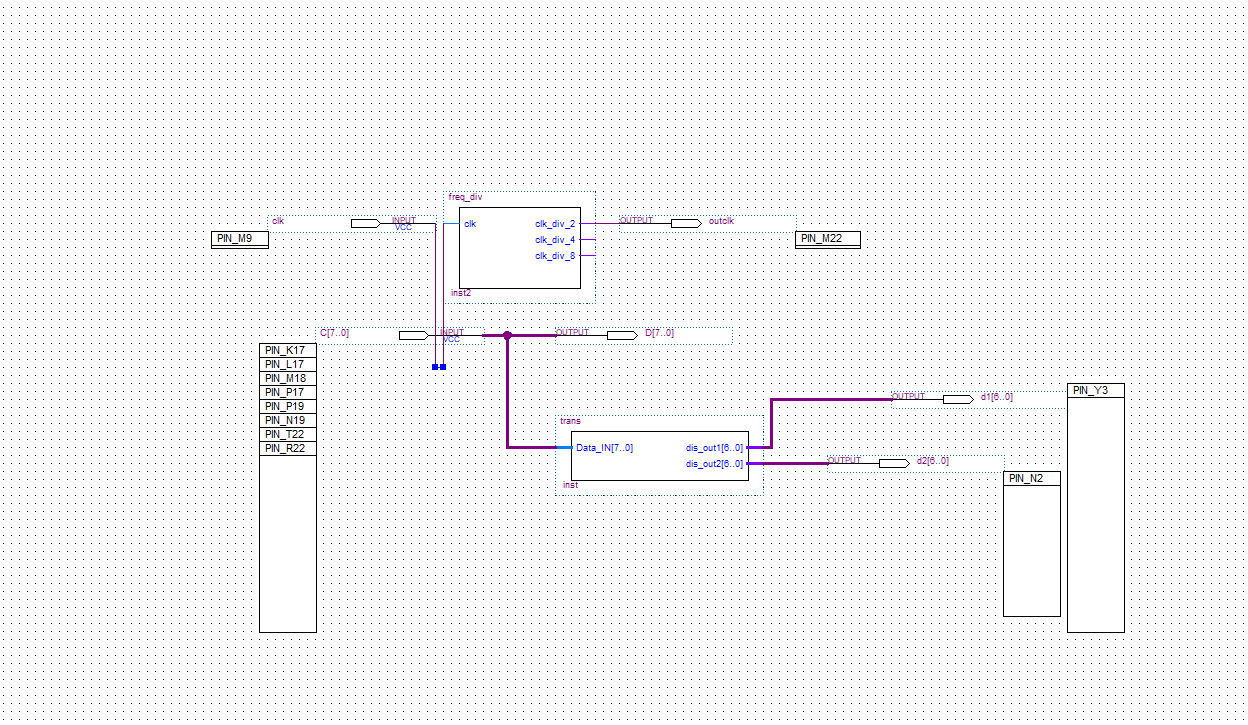
\includegraphics[width=0.75\textwidth]{电路.png}
    \caption{基于 FPGA 的模数转换电路顶层原理图}
    \label{e7:fig:top}
\end{figure}

\section{实验内容}

\subsection{建立工程}

打开 Quartus II，用 \textbf{File $\rightarrow$ New Project Wizard} 新建工程，器件选 DE0-CV 板对应的 Cyclone V \texttt{5CEBA4F23C7}，把顶层实体设为原理图文件 \texttt{top}。随后分别编写两个 VHDL 子模块并绘制顶层原理图。

\subsection{编写分频模块 freq\_div}

\texttt{freq\_div} 用一个 3 位计数器对输入时钟 \texttt{clk} 计数，每个上升沿加 1、计满后归零，再把计数器最低三位分别取反输出 \texttt{clk\_div\_2}、\texttt{clk\_div\_4}、\texttt{clk\_div\_8}，对应二分频、四分频和八分频。本实验取二分频输出 \texttt{clk\_div\_2}，把 50\,MHz 变成 25\,MHz 作 AD9280 的驱动时钟。

\begin{minted}{vhdl}
LIBRARY IEEE;
USE IEEE.STD_LOGIC_1164.ALL;
USE IEEE.STD_LOGIC_ARITH.ALL;
USE IEEE.STD_LOGIC_UNSIGNED.ALL;
ENTITY freq_div IS
PORT (
    clk       : IN  STD_LOGIC;
    clk_div_2 : OUT STD_LOGIC;       -- 二分频，25MHz
    clk_div_4 : OUT STD_LOGIC;       -- 四分频
    clk_div_8 : OUT STD_LOGIC);      -- 八分频
END freq_div;
ARCHITECTURE clk_div_behavior OF freq_div IS
    SIGNAL counter : STD_LOGIC_VECTOR (2 DOWNTO 0);
BEGIN
    PROCESS(clk)
    BEGIN
        IF(clk'EVENT AND clk = '1')THEN
            IF(counter = "111")THEN counter <= "000";
            ELSE counter <= counter + 1;
            END IF;
        END IF;
    END PROCESS;
    clk_div_2 <= NOT counter(0);
    clk_div_4 <= NOT counter(1);
    clk_div_8 <= NOT counter(2);
END clk_div_behavior;
\end{minted}
\captionof{listing}{时钟分频模块 freq\_div.vhd}
\label{e7:lst:freqdiv}

\subsection{编写译码模块 trans}

\texttt{trans} 接收 AD 输出的 8 位数据 \texttt{Data\_IN}，用一段 \texttt{CASE} 组合逻辑把特征值映射成两位数码管的段码 \texttt{dis\_out1}、\texttt{dis\_out2}，实现表~\ref{e7:tab:trans} 的显示。其中 255 显示 \texttt{80}、0 显示 \texttt{39}，其余所有值两位数码管均显示横线 \texttt{==}。

\begin{minted}{vhdl}
library ieee;
use ieee.std_logic_1164.all;
ENTITY trans IS
port (Data_IN  : in  std_logic_vector (7 downto 0);
      dis_out1 : out std_logic_vector (6 downto 0);
      dis_out2 : out std_logic_vector (6 downto 0));
end trans;
ARCHITECTURE fwn OF trans IS BEGIN
PROCESS (Data_IN) BEGIN
CASE Data_IN IS
    WHEN "11111111" => dis_out1 <= "1000000"; dis_out2 <= "0000000"; -- 高电位 80
    WHEN "00000000" => dis_out1 <= "0010000"; dis_out2 <= "0110000"; -- 低电位 39
    WHEN others     => dis_out1 <= "0111110"; dis_out2 <= "0111110"; -- 其他情况显示 ==
END CASE;
END PROCESS;
END fwn;
\end{minted}
\captionof{listing}{显示译码模块 trans.vhd}
\label{e7:lst:trans}

把这两个模块分别编译，再用 \textbf{File $\rightarrow$ Create/Update $\rightarrow$ Create Symbol Files for Current File} 各自生成 \texttt{.bsf} 符号，供顶层原理图调用。

\subsection{绘制顶层原理图}

新建一个 BDF 原理图作为顶层设计，把各模块符号放上去并按下面的关系连线，得到图~\ref{e7:fig:top}。

\begin{itemize}
    \item 输入有两个：\texttt{clk} 接板载 50\,MHz 系统时钟，总线 \texttt{C[7..0]} 接 AD9280 输出的 8 位数据。
    \item \texttt{freq\_div} 以 \texttt{clk} 为输入，二分频输出 \texttt{clk\_div\_2} 接到输出脚 \texttt{outclk}，作为 AD9280 的 25\,MHz 驱动时钟。
    \item 输入总线 \texttt{C[7..0]} 一路直接接输出总线 \texttt{D[7..0]} 驱动 8 位 LED，另一路接 \texttt{trans} 的 \texttt{Data\_IN[7..0]}。
    \item \texttt{trans} 的 \texttt{dis\_out1[6..0]} 接输出 \texttt{d1[6..0]} 驱动第一位数码管，\texttt{dis\_out2[6..0]} 接 \texttt{d2[6..0]} 驱动第二位数码管。
\end{itemize}

\subsection{引脚分配}

把 BDF 设为顶层实体完整编译一遍，再打开 Pin Planner 按表~\ref{e7:tab:pins} 把各端口锁定到 DE0-CV 板和 AD 子板对应的引脚上，引脚配置截图见图~\ref{e7:fig:pin}。其中 \texttt{C[7..0]} 接 GPIO 上 AD 子板的数据口 \texttt{ad\_data[7..0]}，\texttt{outclk} 接 AD 子板的 \texttt{ad\_clk}。

\begin{table}[H]
    \centering
    \caption{引脚分配：端口与 DE0-CV 板载资源及 AD 模块的对应关系}
    \label{e7:tab:pins}
    \begin{tabular}{llll}
        \toprule
        \textbf{端口} & \textbf{方向} & \textbf{引脚} & \textbf{说明} \\
        \midrule
        \texttt{clk}      & 输入 & \texttt{PIN\_M9} & 板载 50\,MHz 系统时钟 \\
        \texttt{C[7..0]}  & 输入 & \texttt{K17,L17,M18,P17,P19,N19,T22,R22} & AD9280 数据 \texttt{ad\_data[7..0]} \\
        \texttt{outclk}   & 输出 & \texttt{PIN\_M22} & 25\,MHz 时钟，接 AD \texttt{ad\_clk} \\
        \texttt{D[7..0]}  & 输出 & \texttt{W2,Y3,N2,N1,U2,U1,L2,L1} & 8 位 LED，显示 AD 数据 \\
        \texttt{d1[6..0]} & 输出 & \texttt{U21,V21,W22,W21,Y22,Y21,AA22} & 第一位数码管 HEX0 \\
        \texttt{d2[6..0]} & 输出 & \texttt{AA20,AB20,AA19,AA18,AB18,AA17,U22} & 第二位数码管 HEX1 \\
        \bottomrule
    \end{tabular}
\end{table}

\begin{figure}[htbp]
    \centering
    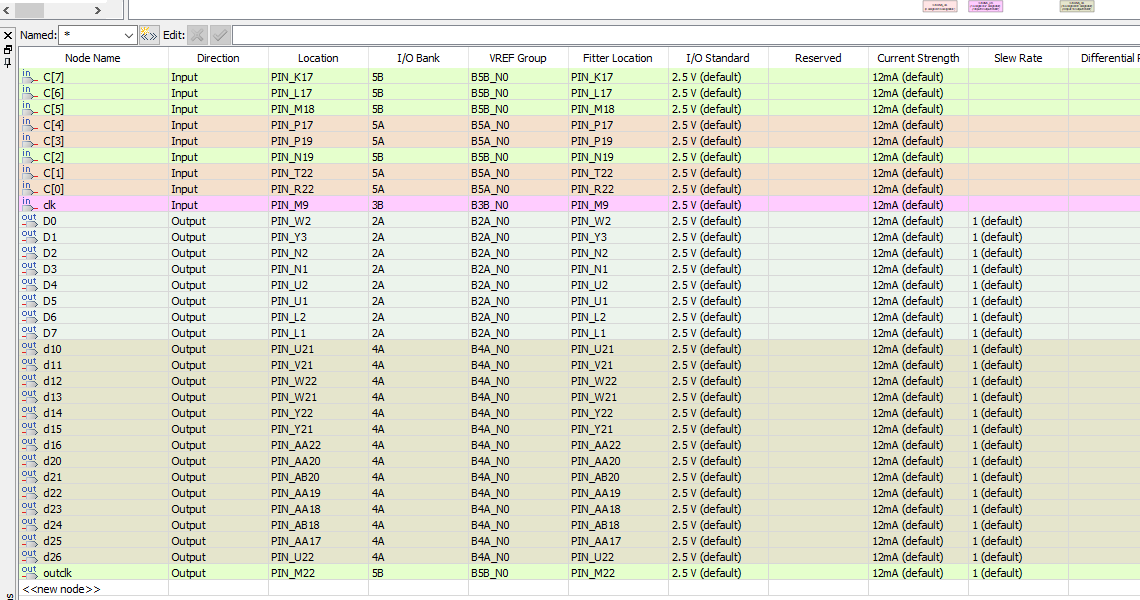
\includegraphics[width=0.75\textwidth]{引脚配置.png}
    \caption{Pin Planner 引脚分配截图}
    \label{e7:fig:pin}
\end{figure}

\subsection{编译与下载}

重新完整编译生成 \texttt{.sof} 配置文件，接上 USB-Blaster，用 JTAG 模式把配置文件下载到 DE0-CV 开发板。

\subsection{接线与测试}

把函数信号源的输出接到 AD 子板的模拟输入端 \texttt{SMA\_IN}，AD 子板的 8 位数据口和 \texttt{ad\_clk} 通过排针接到 FPGA 对应的 GPIO。信号源设为 1\,Hz 方波，先把幅度调到 $\pm5\,$V，再依次减到 $\pm4\,$V、$\pm3\,$V、$\pm2\,$V、$\pm1\,$V，每一档分别在方波的正峰和负峰读出 8 位 LED 显示的二进制数字码，同时观察两位数码管的显示。

\subsection{实验数据}

各档幅度下正负峰电压对应的 8 位数字输出实测值见表~\ref{e7:tab:data}，原始记录见图~\ref{e7:fig:rawdata}。方波幅度为 $\pm5\,$V 时，正峰和负峰对应的数码管显示和 LED 状态见图~\ref{e7:fig:disp} 的 (a) 和 (b)；其他输入幅度下数码管显示横线 \texttt{==}，见图~\ref{e7:fig:disp} 的 (c)。

\begin{table}[H]
    \centering
    \caption{各档幅度下正负峰电压的 8 位数字输出实测值}
    \label{e7:tab:data}
    \begin{tabular}{ccccc}
        \toprule
        \textbf{信号源幅度} & \textbf{峰值电压} & \textbf{LED[7..0] 二进制} & \textbf{十进制} \\
        \midrule
        \multirow{2}{*}{$\pm5\,$V} & $+5\,$V & \texttt{11111111} & 255 \\
                                   & $-5\,$V & \texttt{00000000} & 0   \\
        \midrule
        \multirow{2}{*}{$\pm4\,$V} & $+4\,$V & \texttt{11101111} & 239 \\
                                   & $-4\,$V & \texttt{00010111} & 23  \\
        \midrule
        \multirow{2}{*}{$\pm3\,$V} & $+3\,$V & \texttt{11001101} & 205 \\
                                   & $-3\,$V & \texttt{00110001} & 49  \\
        \midrule
        \multirow{2}{*}{$\pm2\,$V} & $+2\,$V & \texttt{10110011} & 179 \\
                                   & $-2\,$V & \texttt{01001011} & 75  \\
        \midrule
        \multirow{2}{*}{$\pm1\,$V} & $+1\,$V & \texttt{10011001} & 153 \\
                                   & $-1\,$V & \texttt{01100101} & 101 \\
        \bottomrule
    \end{tabular}
\end{table}

\begin{figure}[htbp]
    \centering
    
\includegraphics[width=0.7\textwidth]{数据.jpg}
    \caption{8 位数字输出原始记录}
    \label{e7:fig:rawdata}
\end{figure}

\begin{figure}[htbp]
    \centering
    \begin{subfigure}{0.48\textwidth}
        \centering
        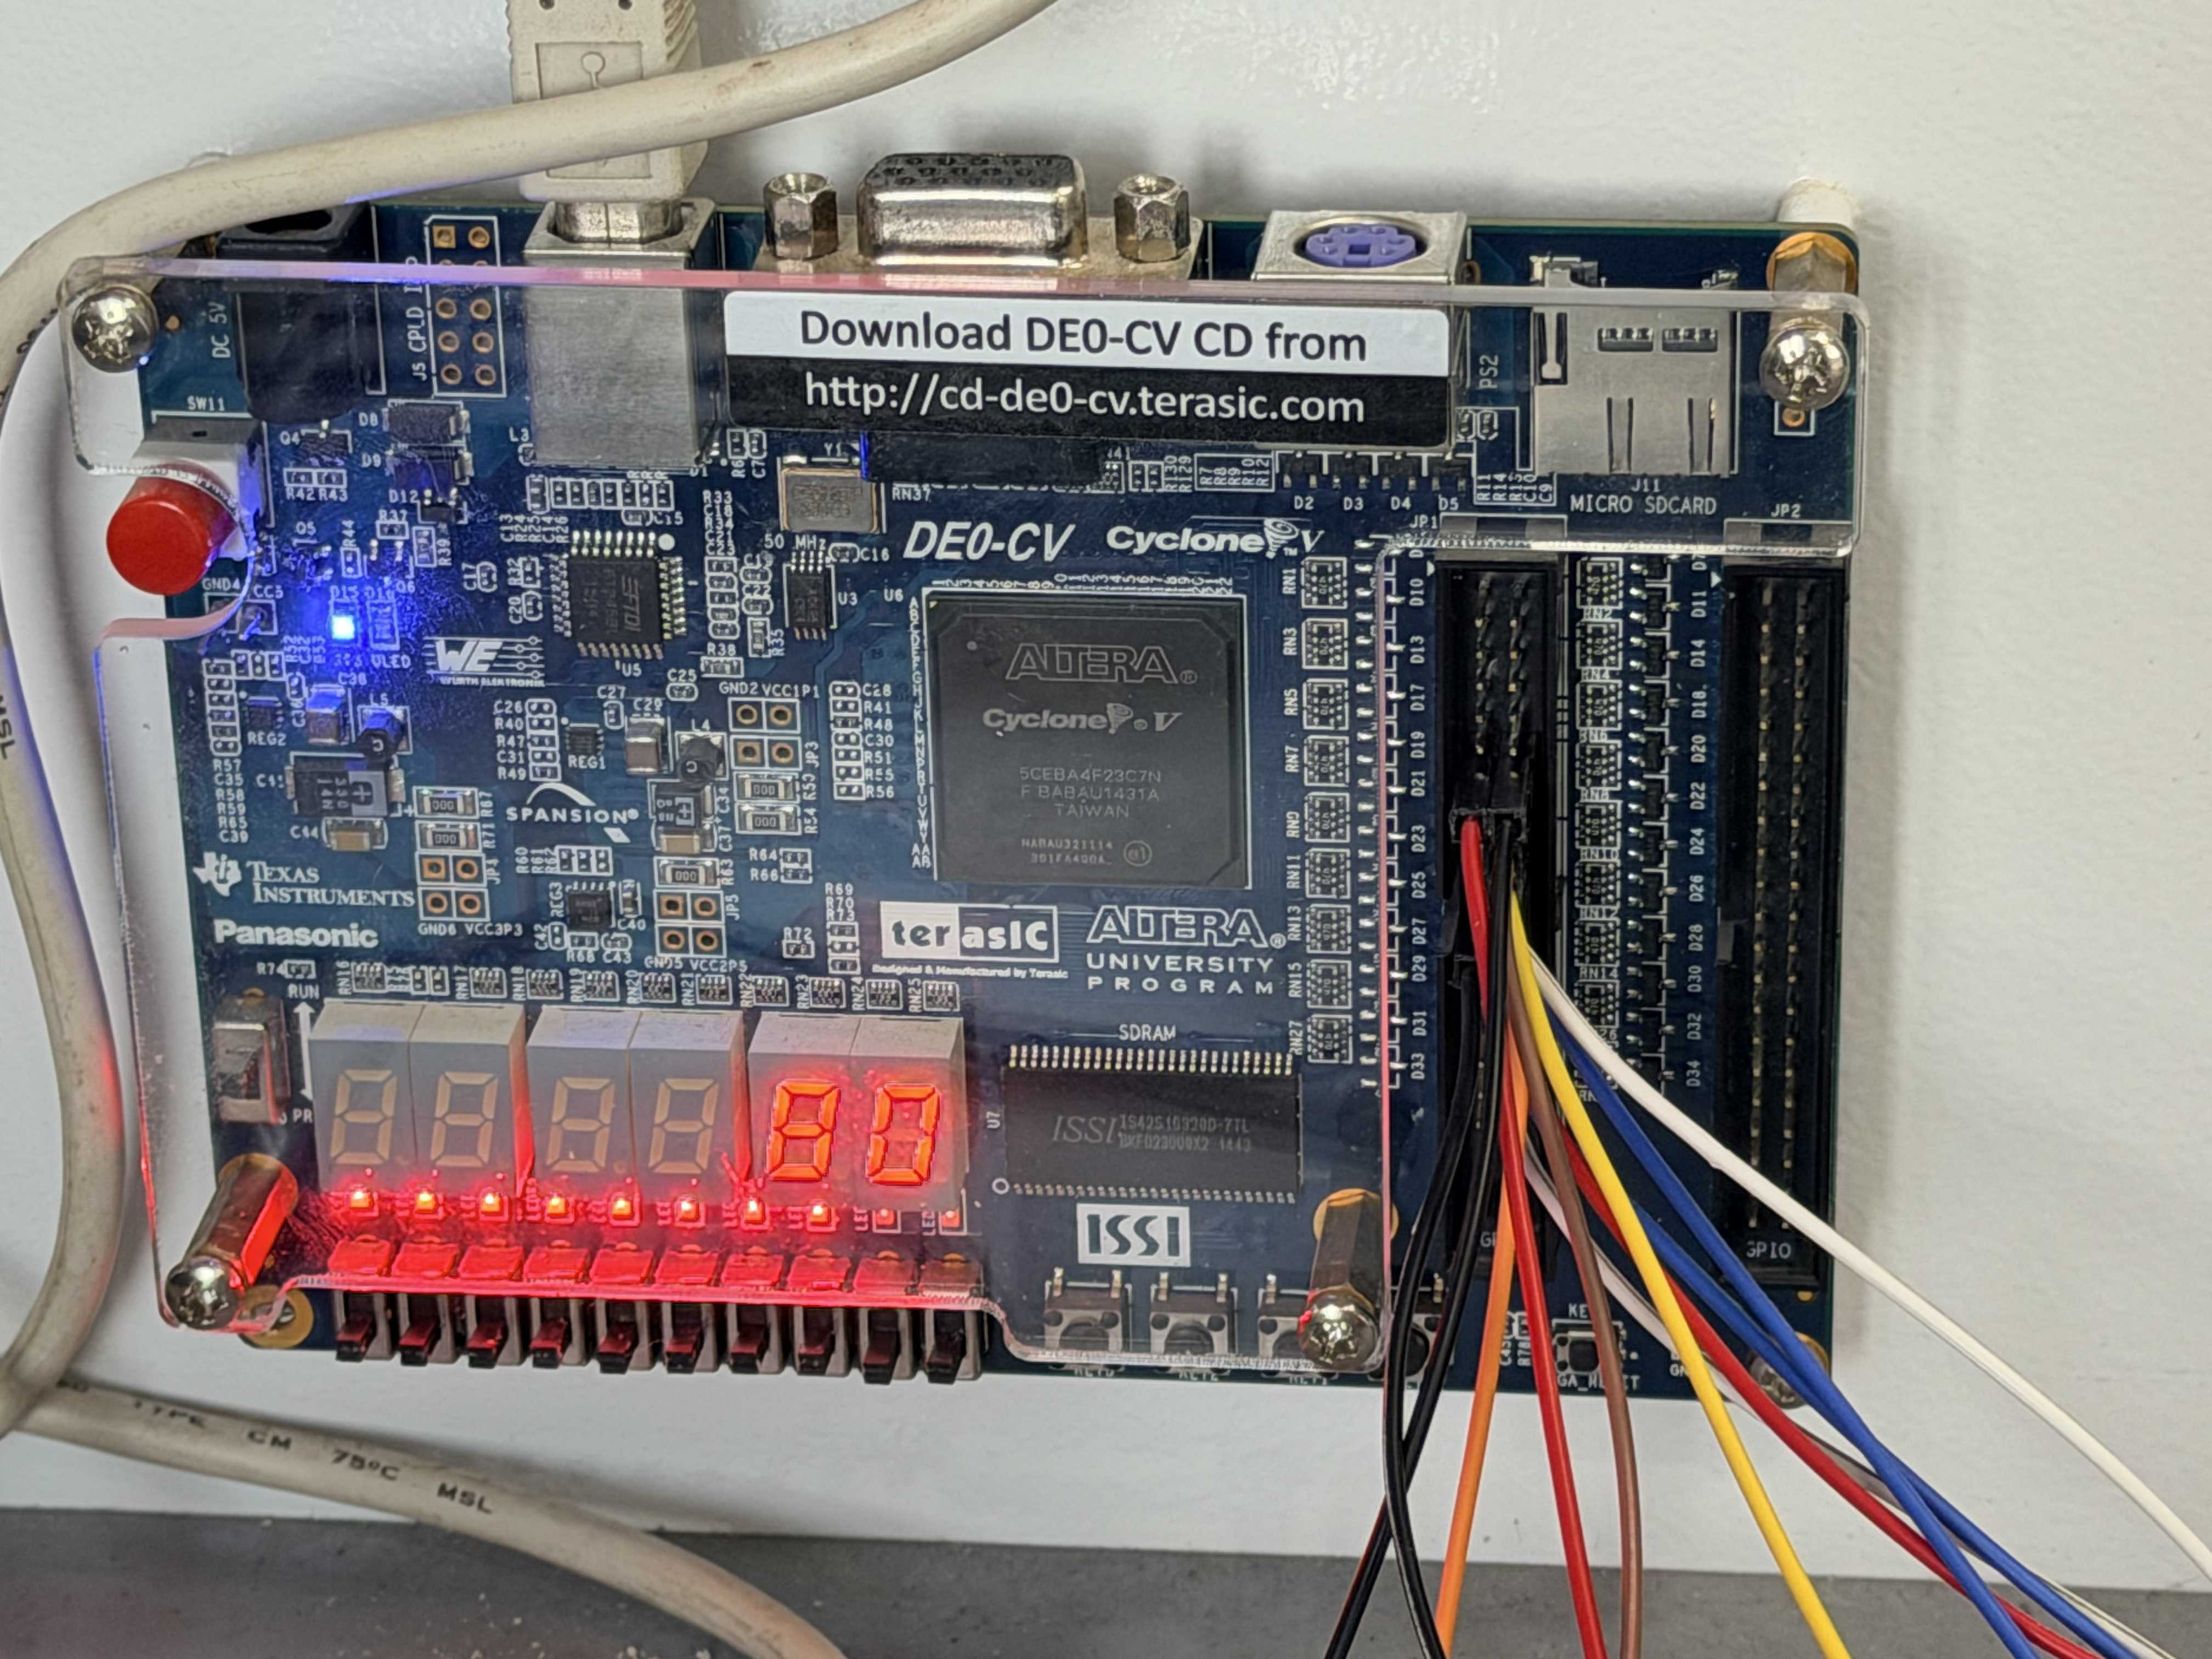
\includegraphics[width=\linewidth]{80.jpg}
        \caption{$+5\,$V，数码管显示 80，LED 全亮}
    \end{subfigure}\hfill
    \begin{subfigure}{0.48\textwidth}
        \centering
        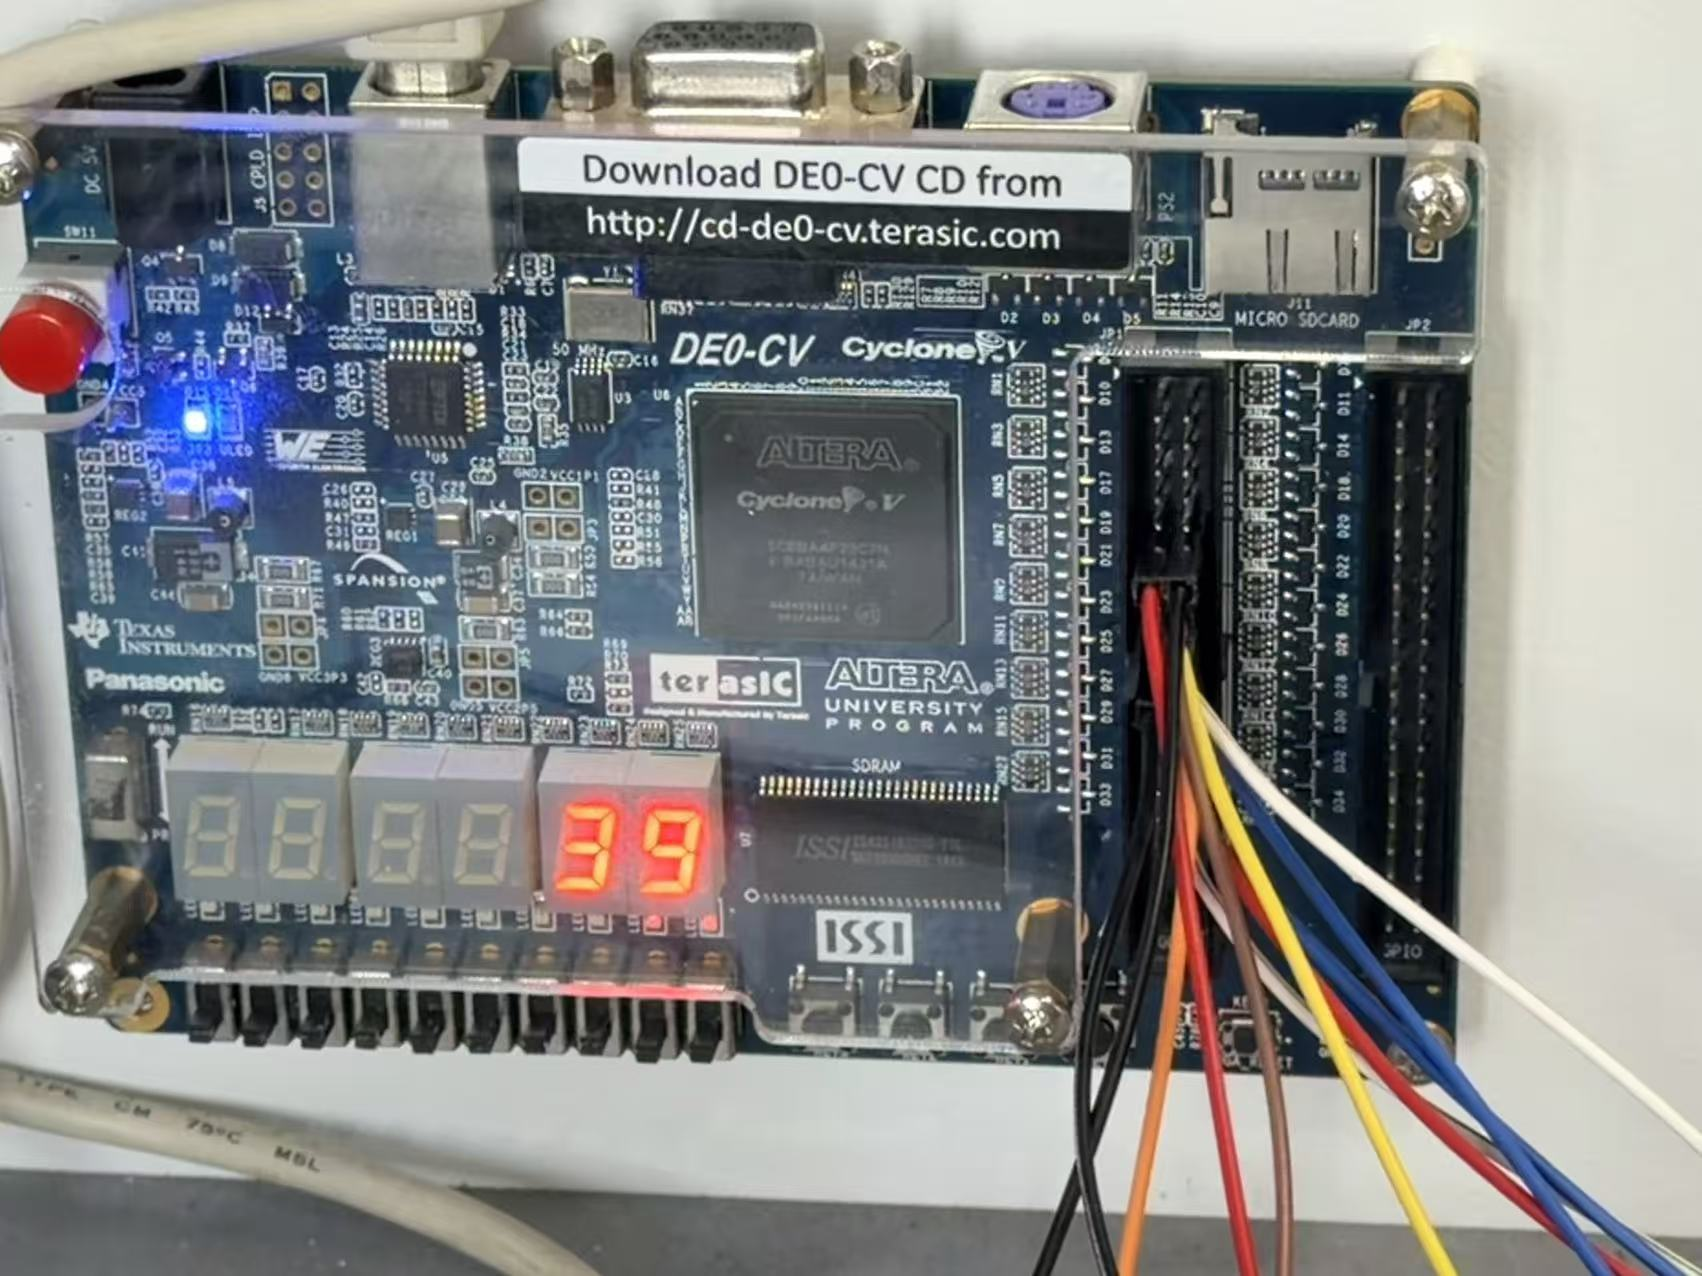
\includegraphics[width=\linewidth]{39.jpg}
        \caption{$-5\,$V，数码管显示 39，LED 全灭}
    \end{subfigure}

    \vspace{6pt}
    \begin{subfigure}{0.6\textwidth}
        \centering
        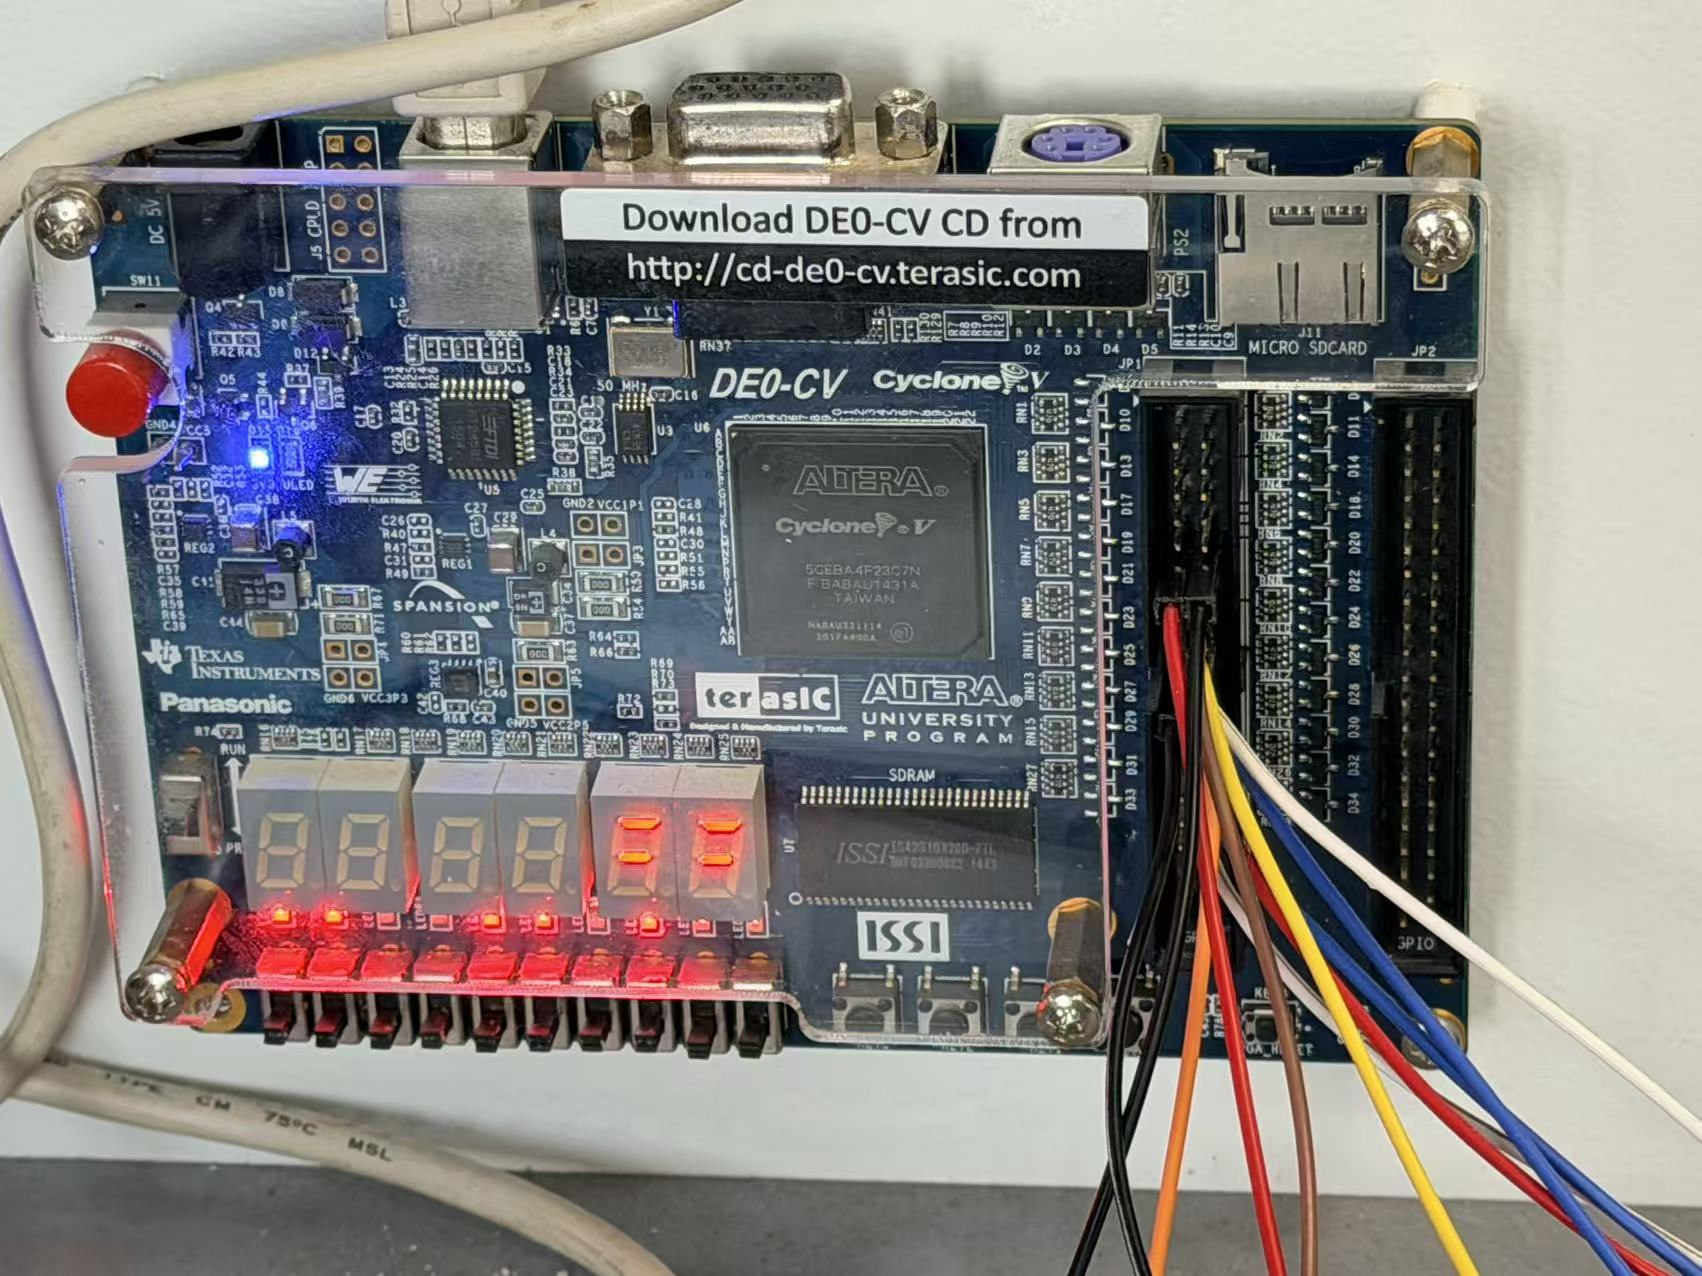
\includegraphics[width=\linewidth]{==.jpg}
        \caption{其他幅度值，数码管显示 \texttt{==}}
    \end{subfigure}
    \caption{两位数码管显示的实测结果}
    \label{e7:fig:disp}
\end{figure}

\subsection{数据分析}

按理论转换式 $D = 25.5\,(V + 5)$ 算出各电压对应的理论数字码，与实测值对照并计算误差，见表~\ref{e7:tab:compare}。

\begin{table}[H]
    \centering
    \caption{实测数字码与理论值对照}
    \label{e7:tab:compare}
    \begin{tabular}{cccc}
        \toprule
        \textbf{峰值电压} & \textbf{理论值} & \textbf{实测值} & \textbf{误差} \\
        \midrule
        $+5\,$V & 255 & 255 & 0   \\
        $-5\,$V & 0   & 0   & 0   \\
        $+4\,$V & 230 & 239 & $+9$ \\
        $-4\,$V & 26  & 23  & $-3$ \\
        $+3\,$V & 204 & 205 & $+1$ \\
        $-3\,$V & 51  & 49  & $-2$ \\
        $+2\,$V & 179 & 179 & 0   \\
        $-2\,$V & 77  & 75  & $-2$ \\
        $+1\,$V & 153 & 153 & 0   \\
        $-1\,$V & 102 & 101 & $-1$ \\
        \bottomrule
    \end{tabular}
\end{table}

对照可以看出，实测数字码与理论值整体吻合很好，除 $+4\,$V 档误差约 9 个最低有效位外，其余各档误差都在 3 个最低有效位以内。利用衰减电路的线性关系还可以做一个对称性检验：同一档正负峰的数字码理论上应满足 $D(+V) + D(-V) = 255$。实测中 $\pm3\,$V、$\pm2\,$V、$\pm1\,$V 三档的正负峰之和都为 254，与 255 仅差一个量化位，进一步印证了转换的线性度。

误差主要来自几个方面：信号源幅度旋钮的读数和实际输出本身有偏差，尤其手动调幅度时不易精确停在整伏；衰减电路的电阻和基准电压存在容差，使比例和平移略偏离理想值；AD9280 是 8 位量化，满量程 $10\,$V 对应 256 级，每级约 $39\,$mV，本身就有约一个最低有效位的量化误差；再加上方波峰值的人工读数误差。这些因素叠加在一起，使个别档位出现几个最低有效位的偏差，属正常范围。

数码管显示方面，$+5\,$V 时正确显示 \texttt{80}、$-5\,$V 时正确显示 \texttt{39}，分别对应两名组员学号的后两位；其他所有输入幅度下均显示横线 \texttt{==}，与译码模块 \texttt{trans} 的设计要求一致。综合数字码和数码管两方面的结果，模数转换、时钟分频和显示译码三部分都工作正常，验证了系统设计的正确性。

\section{实验过程中的问题}

\begin{enumerate}
    \item \textbf{驱动时钟必须分频}。AD9280 的最大转换时钟只有 32\,MHz，直接用 50\,MHz 板载时钟会超过上限导致转换不稳定。解决办法是用 \texttt{freq\_div} 把 50\,MHz 二分频成 25\,MHz，再通过 \texttt{outclk} 引脚送给 AD9280 作驱动时钟。
    \item \textbf{AD 数据线位序的对应}。AD9280 的数据口 \texttt{ad\_data[7..0]} 要和 FPGA 输入总线 \texttt{C[7..0]} 一一对应，如果高低位接反，读出的数字码会变成镜像，电压和数据的对应关系全乱。接线时按表~\ref{e7:tab:pins} 的引脚逐根核对，确认低位对低位、高位对高位。
    \item \textbf{衰减电路的电压标定}。外部 $-5\,$V 至 $+5\,$V 必须经子板衰减电路变成 $0\,$V 至 $2\,$V 才能进 AD9280，关系是 $\mathrm{AD\_IN2} = \mathrm{SMA\_IN}/5 + 1$。一开始没注意这级衰减，按 $0\,$V 至 $5\,$V 估算数据对不上，弄清衰减关系后理论值才和实测吻合。
    \item \textbf{译码特征值与学号的对应}。\texttt{trans} 里要把 255 译码成 \texttt{80}、把 0 译码成 \texttt{39}，调试时容易把两个数码管的段码或两名同学的学号对调，需要对照表~\ref{e7:tab:trans} 逐一核对段码，并在 $+5\,$V 和 $-5\,$V 两种状态下实测确认显示正确。
\end{enumerate}

\section{心得体会}

\begin{enumerate}
    \item 这次实验让我把模数转换的完整链路理解透彻了。从信号源的模拟方波，到衰减电路把 $\pm5\,$V 映射进 AD9280 的量程，再到芯片量化输出 8 位数字码，最后用 LED 和数码管显示，我清楚地看到了一个连续的模拟量是怎样一步步变成离散数字量的，也体会到衰减电路和量化精度对结果的直接影响。
    \item 时钟分频这个环节看似简单，却很关键。正是因为 AD9280 有 32\,MHz 的时钟上限，才必须先把 50\,MHz 分频，这让我意识到接口芯片的时序约束在系统设计里不能忽视，时钟规划要从一开始就考虑进去。
    \item 整个系统是 VHDL 文本设计与原理图设计的结合：分频和译码的逻辑用 VHDL 描述更清晰，各模块之间怎么连用原理图看得更直观。把它们生成符号再在顶层拼起来，配合外接 AD 模块和信号源测试，我完整走通了从数字设计到模数转换、再到结果显示的全过程，对数字系统的整体开发流程熟悉了不少。
\end{enumerate}

\end{document}
